\chapter{GRIEEL Transition Algorithm}
\label{ch:chapter_five}%

This chapter introduced the principal contribution of this research, which has inspired the BME theory (discussed in \ref{sec:base_manipolability}). 
The tools to model, control, and analyze the performance of multi-limbed robots, and the description of LIMBERO-GRIEEL (L-G) are fundamental for defining an efficient transformation algorithm.

The multimodal locomotion capabilities of L-G require a seamless transition between two functional modes:  a wheeled locomotion system and a versatile gripper for manipulation and walking/climbing tasks.
Furthermore, hybrid configurations are considered, such as limbs in wheel mode used for driving and others in gripper mode to manipulate the environment and carry objects. 

The final objective is the definition of an efficient and stable algorithm to perform the transition of locomotion mode for L$-$G, in terms of motion planning and control. 

Additionally, the reusability and modularity of this procedure have been an additional requirement. 
In fact, GRIEEL's potential goes beyond its usage as LIMBERO's EE, making its design, control system, and related procedure adaptable for any limbed robotic system is the ultimate goal.   

First, the previous procedure used to perform this locomotion transition is described, and the limitations are discussed. 
Then, the new algorithm is defined, and the base motion sequence is analyzed using the novel BVME. 
Finally, the advantages of the proposed algorithm are highlighted. 
The higher-level components that decide when and what type of transition is needed goes behind this research, in any case, once developed are easy to integrate on the system. 

\section{Previous Transformation Procedure}
\label{sec:old_algorithm}

The procedure defined by M.Uda\cite{GRIEELUdaThesis} to perform locomotion mode transition is reported in Fig\ref{fig:GRIEEL_oldTransition}, with the relative timeline.
This motion sequence, responsible for the driving-to-walking locomotion transition, starts at $t=20s$ and ends at $t=120$, with the following steps: 
\begin{enumerate}
    \setlength\itemsep{-0.7em} 
    \item\label{item:old_1} Lay the base on the ground.
    \item\label{item:old_2} Complete W2G transition for all modules, releasing tethers tension. 
    \item\label{item:old_3} Raise all the limbs 
    \item\label{item:old_4} change wrist configuration. 
    \item\label{item:old_5} Stand up, maintaining the LF leg raised, ready for walking. 
\end{enumerate}
The opposite walking-to-driving transition is defined with a similar sequence, except for steps (\ref{item:old_3}) and (\ref{item:old_5}). In (\ref{item:old_3}) a different wrist configuration is defined in the case of module G2W transition.For step (\ref{item:old_5}), if driving is the upcoming locomotion mode, all limbs (in wheel mode) are kept in contact with the ground. 
\begin{figure}[H]
    \centering
    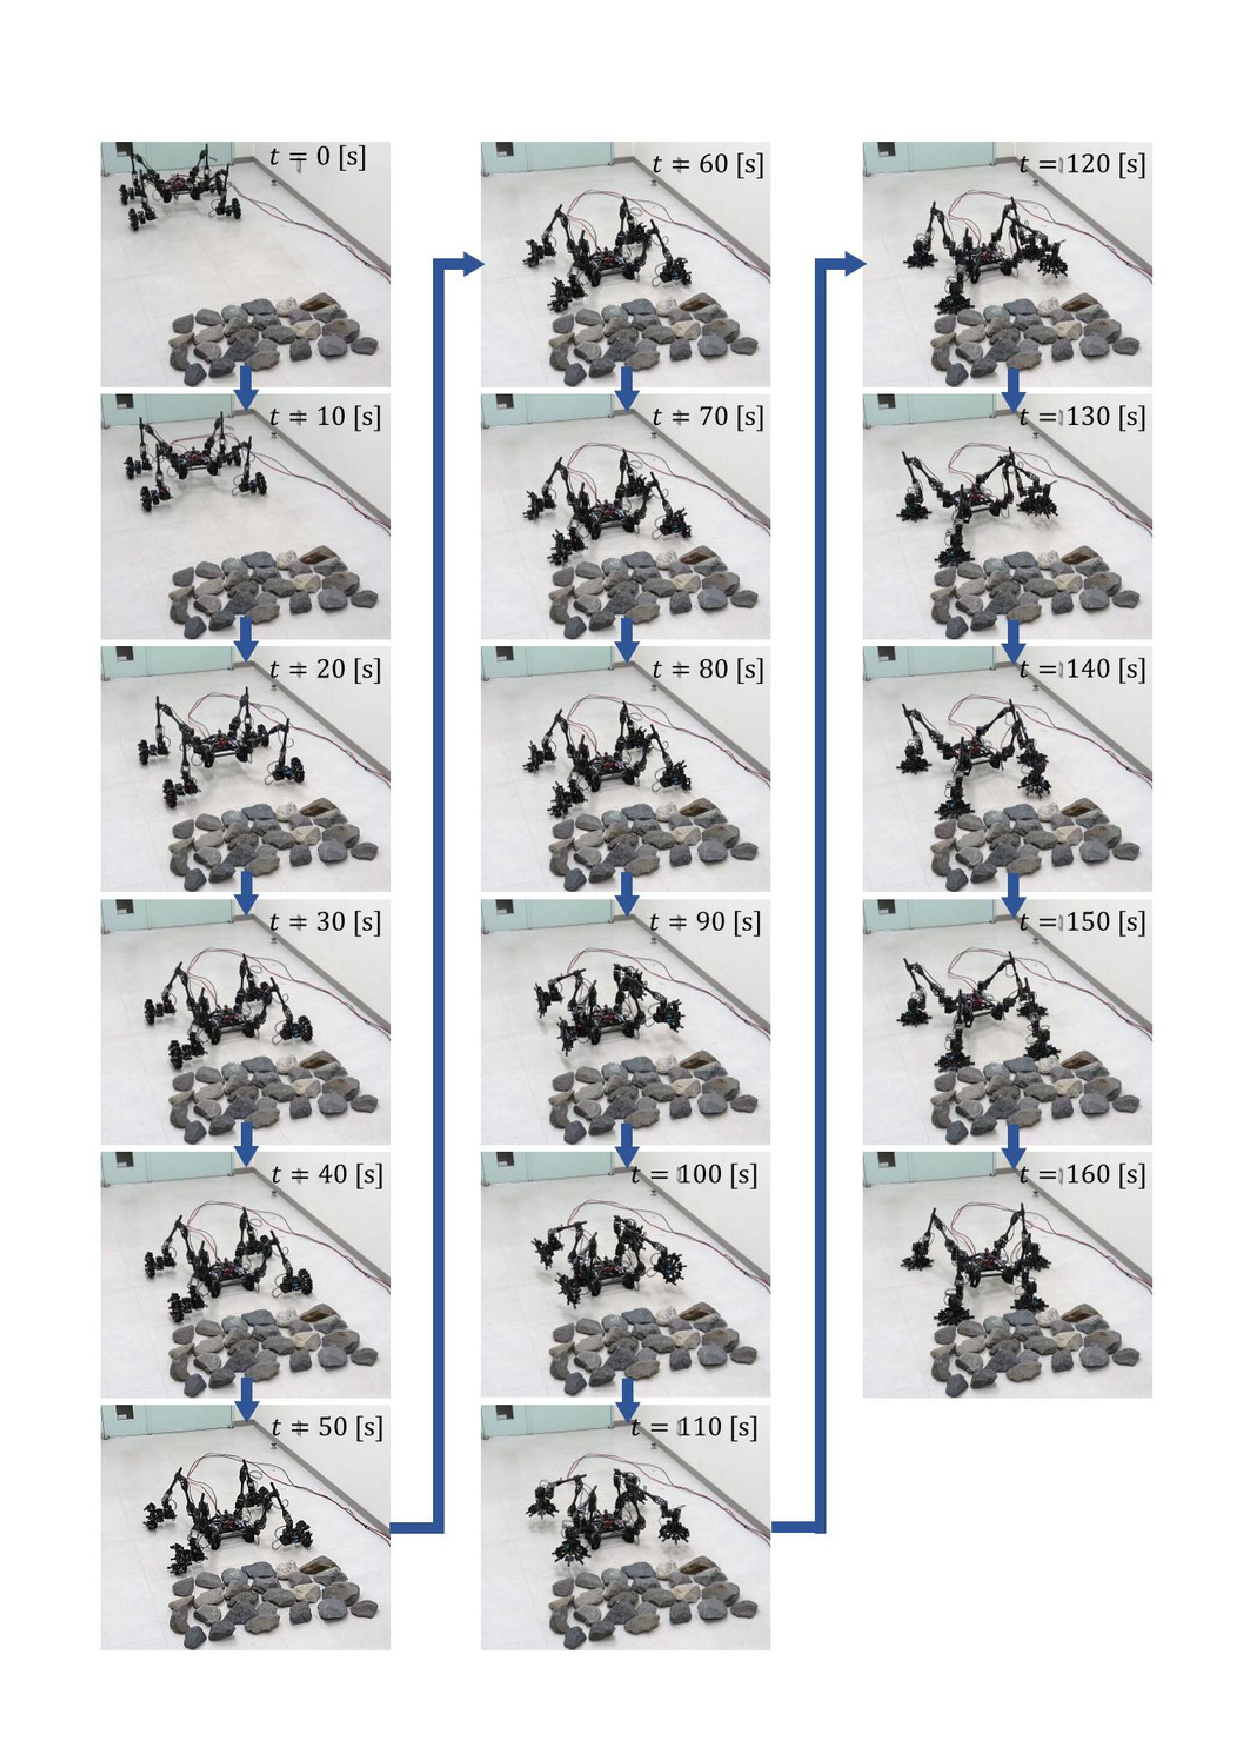
\includegraphics[width=0.65\textwidth]{Images/img_ch5/GRIEEL_oldTransition.pdf}
    \caption{\cite{GRIEELUdaThesis}Driving to walking locomotion transition with the previous algorithm (transformation of all limbs W2G).}
    \label{fig:GRIEEL_oldTransition}
\end{figure}
This sequence is completed in a small amount of time, with reduced energy consumption, and is easy to define. However, it has the following limitations:
\begin{itemize}
    \setlength\itemsep{-0.7em} 
    \item[\textbf{a)}] \label{item:problem_a} A horizontal support plane is required when laying down the base, to avoid any possible tumbling problems. Furthermore, unexpected rocks or small sharp obstacles could damage the bottom of the base, where batteries and other electronics are exposed (One possible solution to this could be a redesign of the robot base. However, this is against the reusability requirements described previously).   
    \item[\textbf{b)}] \label{item:problem_b} It is not the best sequence for a single-limb transformation. In a transition to a hybrid configuration, as changing from full driving locomotion (4-wheeled) to 3-wheeled with one manipulating gripper, this procedure is time-consuming and not always possible. 
    
    Another case when a single transformation is needed is transitioning during locomotion. This means that the gait scheduler is involved in the transition, instead of maintaining the same pose in space during mode transformation, it is completed while moving towards the objective. This is not discussed here, but some comments are made in the last section.  
\end{itemize}

The new motion sequence is now defined, to overcome those problems and guarantee the requirements listed before. 

\section{New Transformation Algorithm}
\label{sec:new_algorithm}

In defining a new transition sequence for GRIEEL, the requirements are: 
\begin{enumerate}
    \setlength\itemsep{-0.7em} 
    \item\label{item:stability} Stability of the system. 
    \item\label{item:rough} Enabling transition even in rough terrains\\(where laying down the base may be not possible). 
    \item\label{item:slopes} Enabling transition in small sloped terrains \\(where GRIEEL's spine gripping can be exploited).
    \item\label{item:reusability} Simple to be redefined and adapted for different conditions or robotic platforms. 
    \item\label{item:single} Possibility to complete single module transitions. 
    \item\label{item:dexterity} Avoid limb configurations where the robot base's dexterity and maneuverability are degraded. 
\end{enumerate}

If all of them are respected in the definition of a new procedure, problems \hyperref[item:problem_a]{(\textbf{a})} and \hyperref[item:problem_b]{(\textbf{b})} are overcome, and the additional desired goals listed in this chapter's introduction are met. 

In this analysis, it is assumed that, when a GRIEEL mode transition is required, the terrain is flat or with small slopes, but rocks and sharp obstacles on the ground can be present. Under this assumption, SP and ZMP criteria can be used to evaluate system stability. The last section of this chapter briefly discusses possible extensions, and how simple it is to integrate them.

The main idea behind the new algorithm comes from the configuration represented in Fig.\ref{fig:limbero_grieel_mars_stable}, as an obvious solution to problem \hyperref[item:problem_a]{(\textbf{a})}. Instead of laying down the base, it is kept above the ground and the limbs' modules are transformed one by one. If this sequence is properly implemented, the "one-by-one" aspect solves also problem \hyperref[item:problem_b]{(\textbf{b})}, enabling single transformation commands. 
\begin{figure}[H]
    \centering
    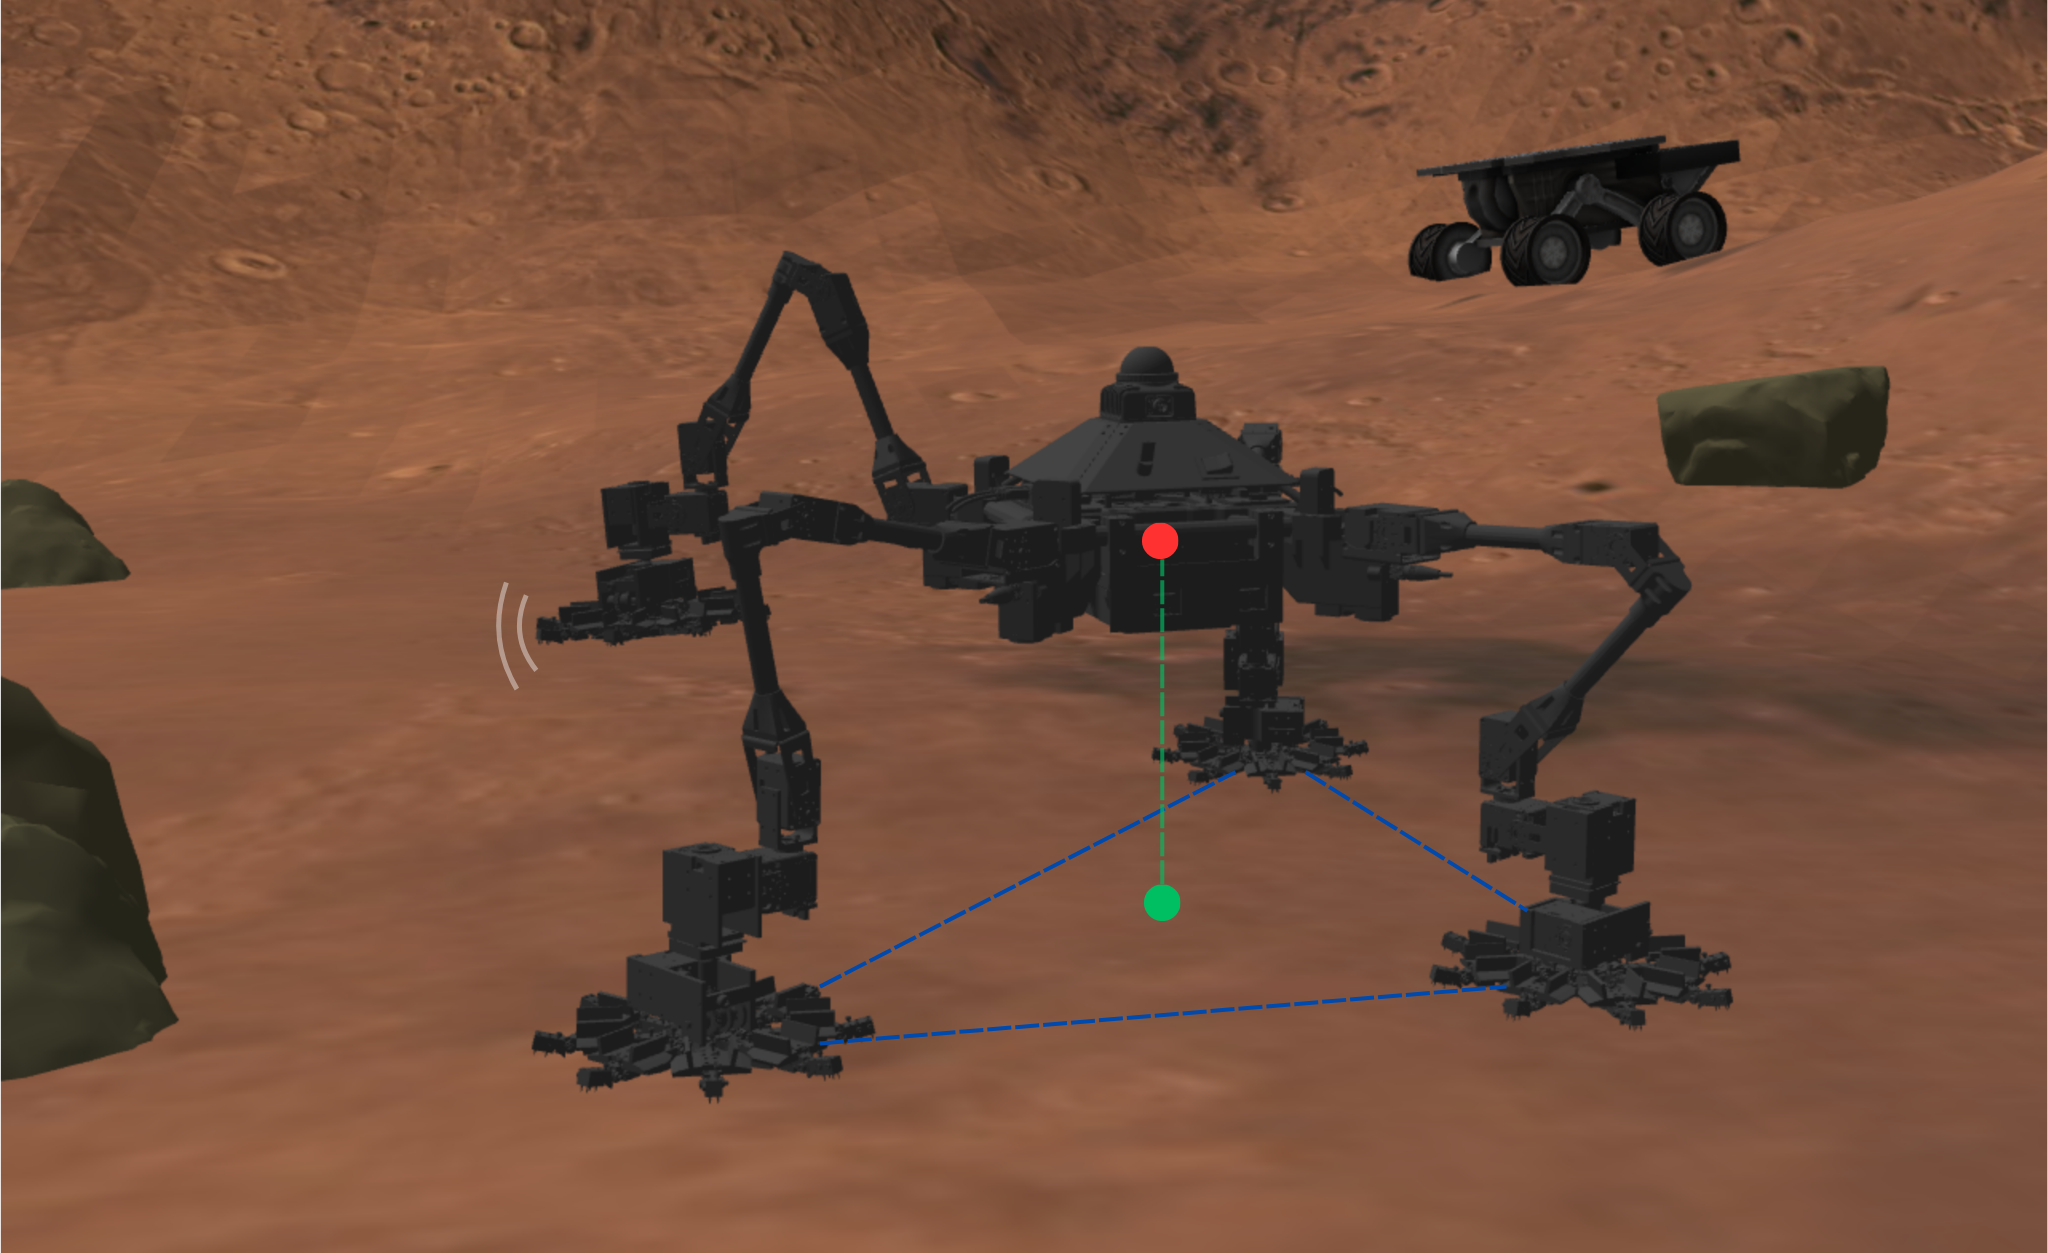
\includegraphics[width=0.5\textwidth]{Images/img_ch5/alg_idea.png}
    \caption{LIMBERO-GRIEEL in a stable configuration ready for single limb transition.}
    \label{fig:limbero_grieel_mars_stable}
\end{figure}
With this approach, the overall mode transformation is decomposed into single-limb problems, and addressing this involves multi-limbed robot stability. 
It is important to note that when GRIEEL goes under a W2G or G2W transition, in both cases ground contact is not admissible, because during the wrist's joints reconfiguration ground sliding may affect the overall structure or damage the module itself. For this reason, any module mode change involves rising up the corresponding limb and maintaining it for the whole transition time. 

For this reason, during a single module transition, LIMBERO-GRIEEL stands on the remaining three limbs, which are responsible for maintaining a stable configuration while the limb is not in contact.

From now on, the algorithm is described for the quadruped robot LIMBERO-GRIEEL used in this research, but some aspects of the extension for N-limbed robots are discussed in the last section. The notation and symbols introduced in the previous chapters are used with the same meaning. 

The type of problem discussed above is a common problem when planning a static gait\cite{McGhee}\cite{Todd}\cite{Raibert}\cite{HiroseDesignGate}, where a stable base CoM positioning is involved during each walking step 
(Dynamic gaits such as trotting\cite{Raibert} are faster but involve an unstable condition during walking locomotion, so they are not considered here).  

The motion sequence to transform limb $j \in J$ can be described at a high level in the following steps: 
\begin{enumerate}
    \setlength\itemsep{-0.7em} 
    \item\label{item:single_1} Select the limb to transform, $j$.  
    \item\label{item:single_2} move the base in a stable configuration for the upcoming limb lift.
    \item\label{item:single_3} lift limb $j$. 
    \item\label{item:single_4} Transform limb $j$ (G2W/W2G).
    \item\label{item:single_5} lay down limb $j$ in the new mode.
\end{enumerate}

The single transition sequence is simple, but step (\ref{item:single_2}) has to be properly defined to give motion commands to the robot, and the "stable base configuration" problem has infinite solutions. If the SSM criterion is used, according to theorem \ref{th:static_stability}, all the feasible configurations where the base CoM projects inside the SP (a continuous space) are fine. 

An approach similar to base positioning for static walking could be used, positioning the base CoM by maximizing the SSM (or an equivalent ZMP margin). This ensures robust stability, but as discussed when introducing the BME (see  chapter\ref{sec:base_manipolability}), it may cause not dexterous configuration, especially for multi-limbed robots that use their body to manipulate objects in the environment.
Another approach also used for gait generation is to ensure a positive SSM, without maximizing it. This gives a lot of freedom, and it is the approach used here and implemented with a simple rule of thumb. 

Multi-limbed robots are young robotic systems, where full autonomy is still under development and research, for this reason, techniques for optimal configurations with a multipurpose view do not exist.\\
A rule of thumb is used here in terms of stability, but it is clear that when LIMBERO-GRIEEL performs a single W2G transition, sample collecting may be the next task, so having the base ready to do it enables better maneuverability and efficiency. This reason gave birth to the BME.

\begin{figure}[H]
    \centering
    \subfloat[$j=LF$, Upcoming support polygon\label{fig:translation1_ex1}]{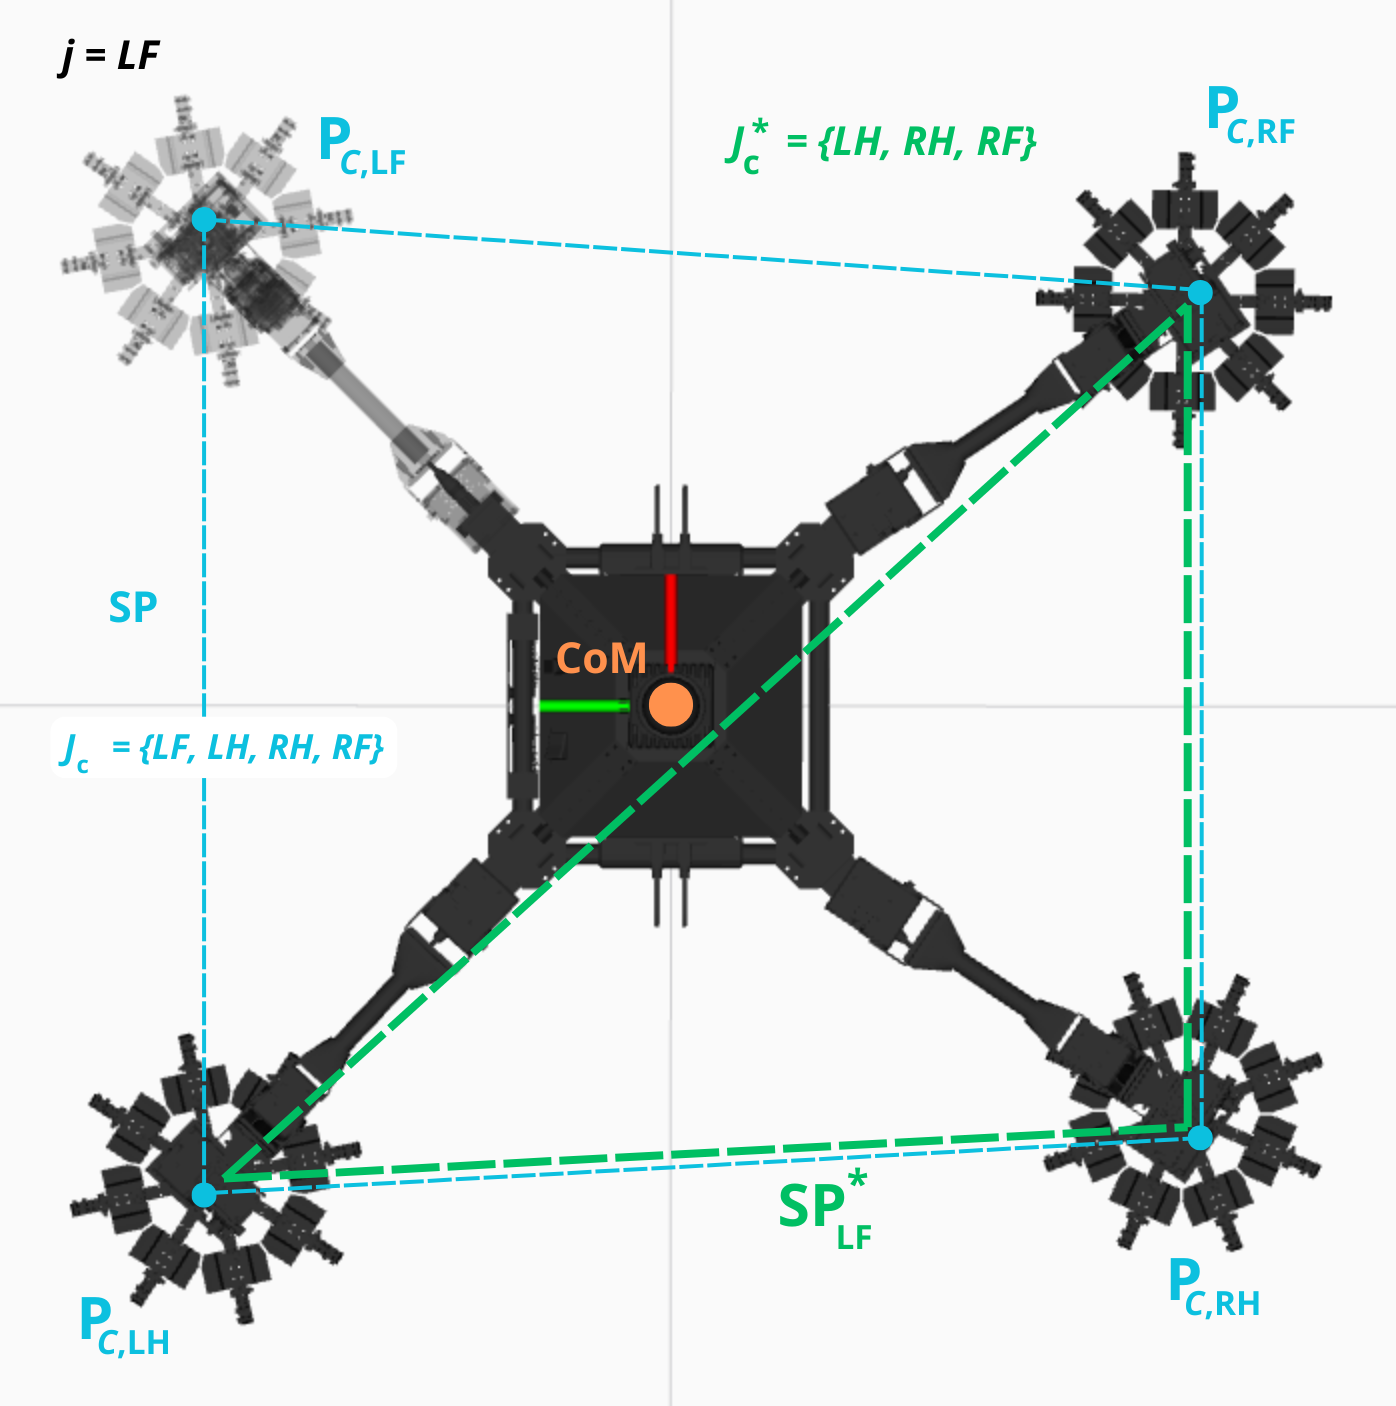
\includegraphics[width=0.3\textwidth]{Images/img_ch5/translation1_ex1.png}} \quad 
    \subfloat[Involved vectors\label{fig:translation2_ex1}]{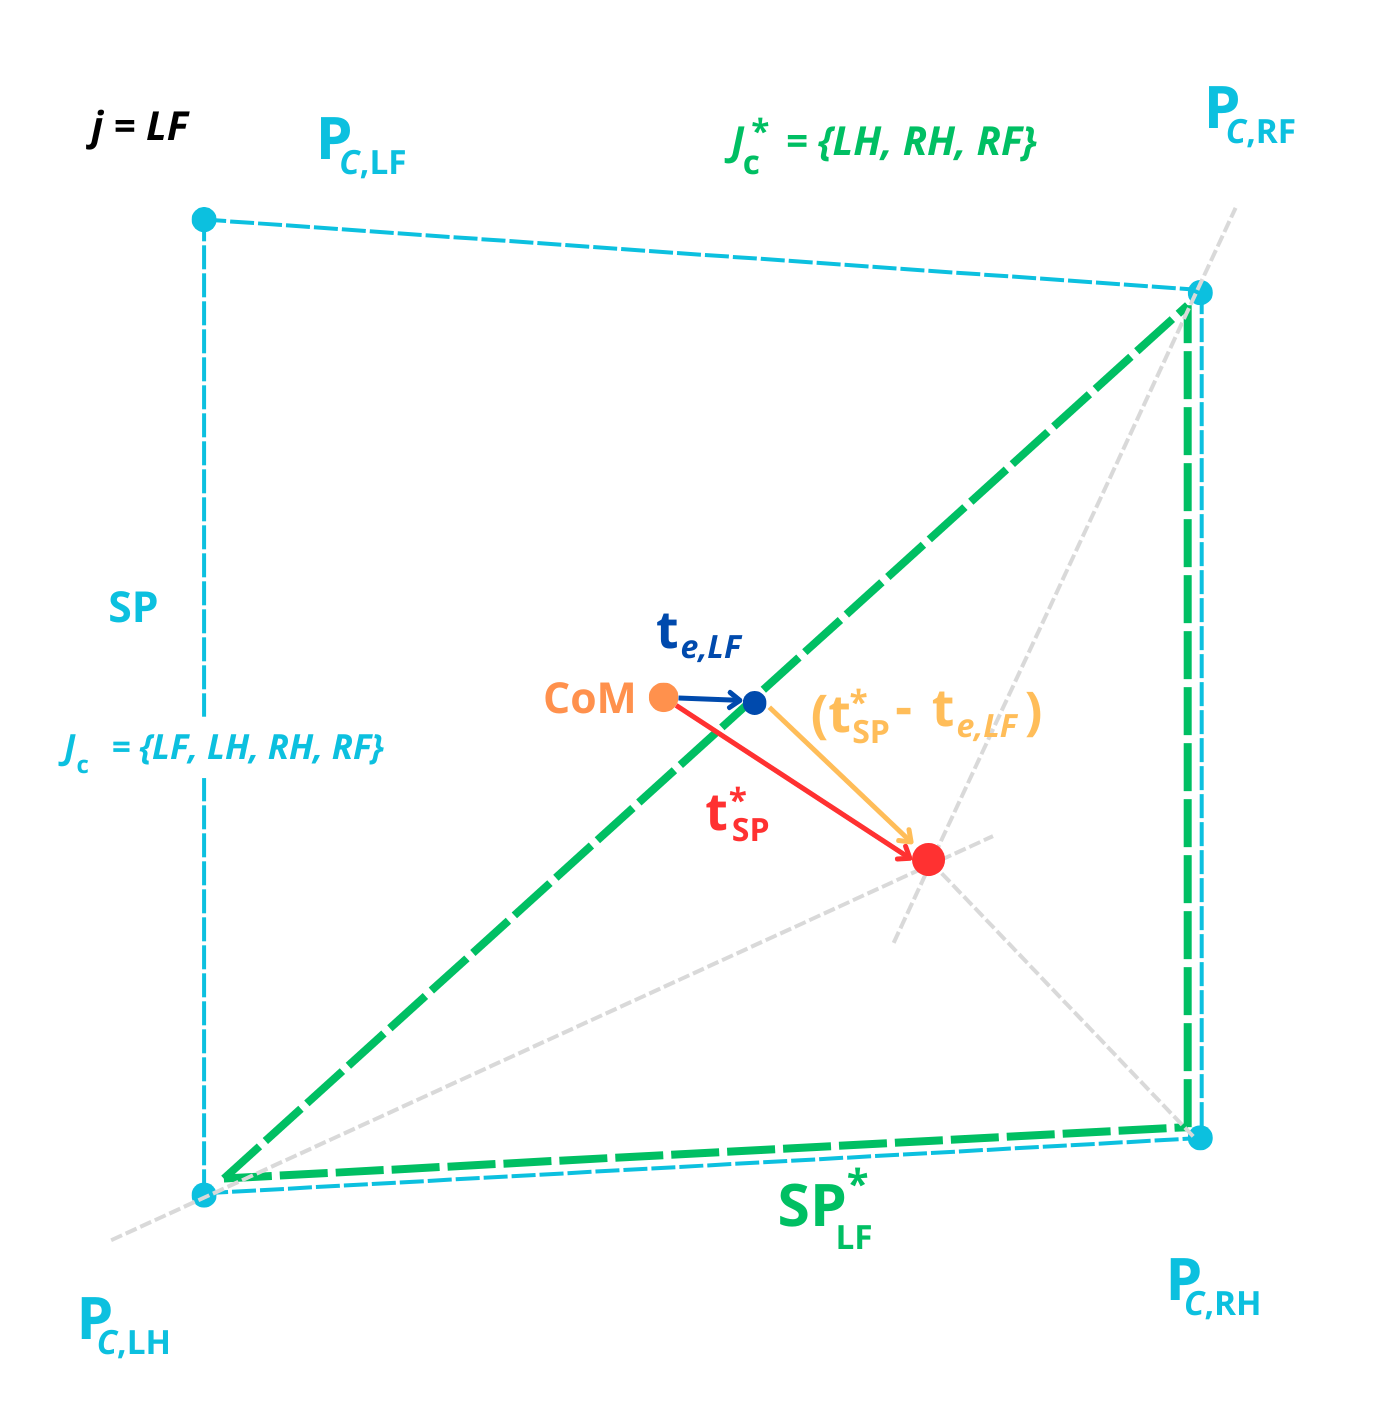
\includegraphics[width=0.3\textwidth]{Images/img_ch5/translation2_ex1.png}} \quad
    \subfloat[Final base translation\label{fig:translation3_ex1}]{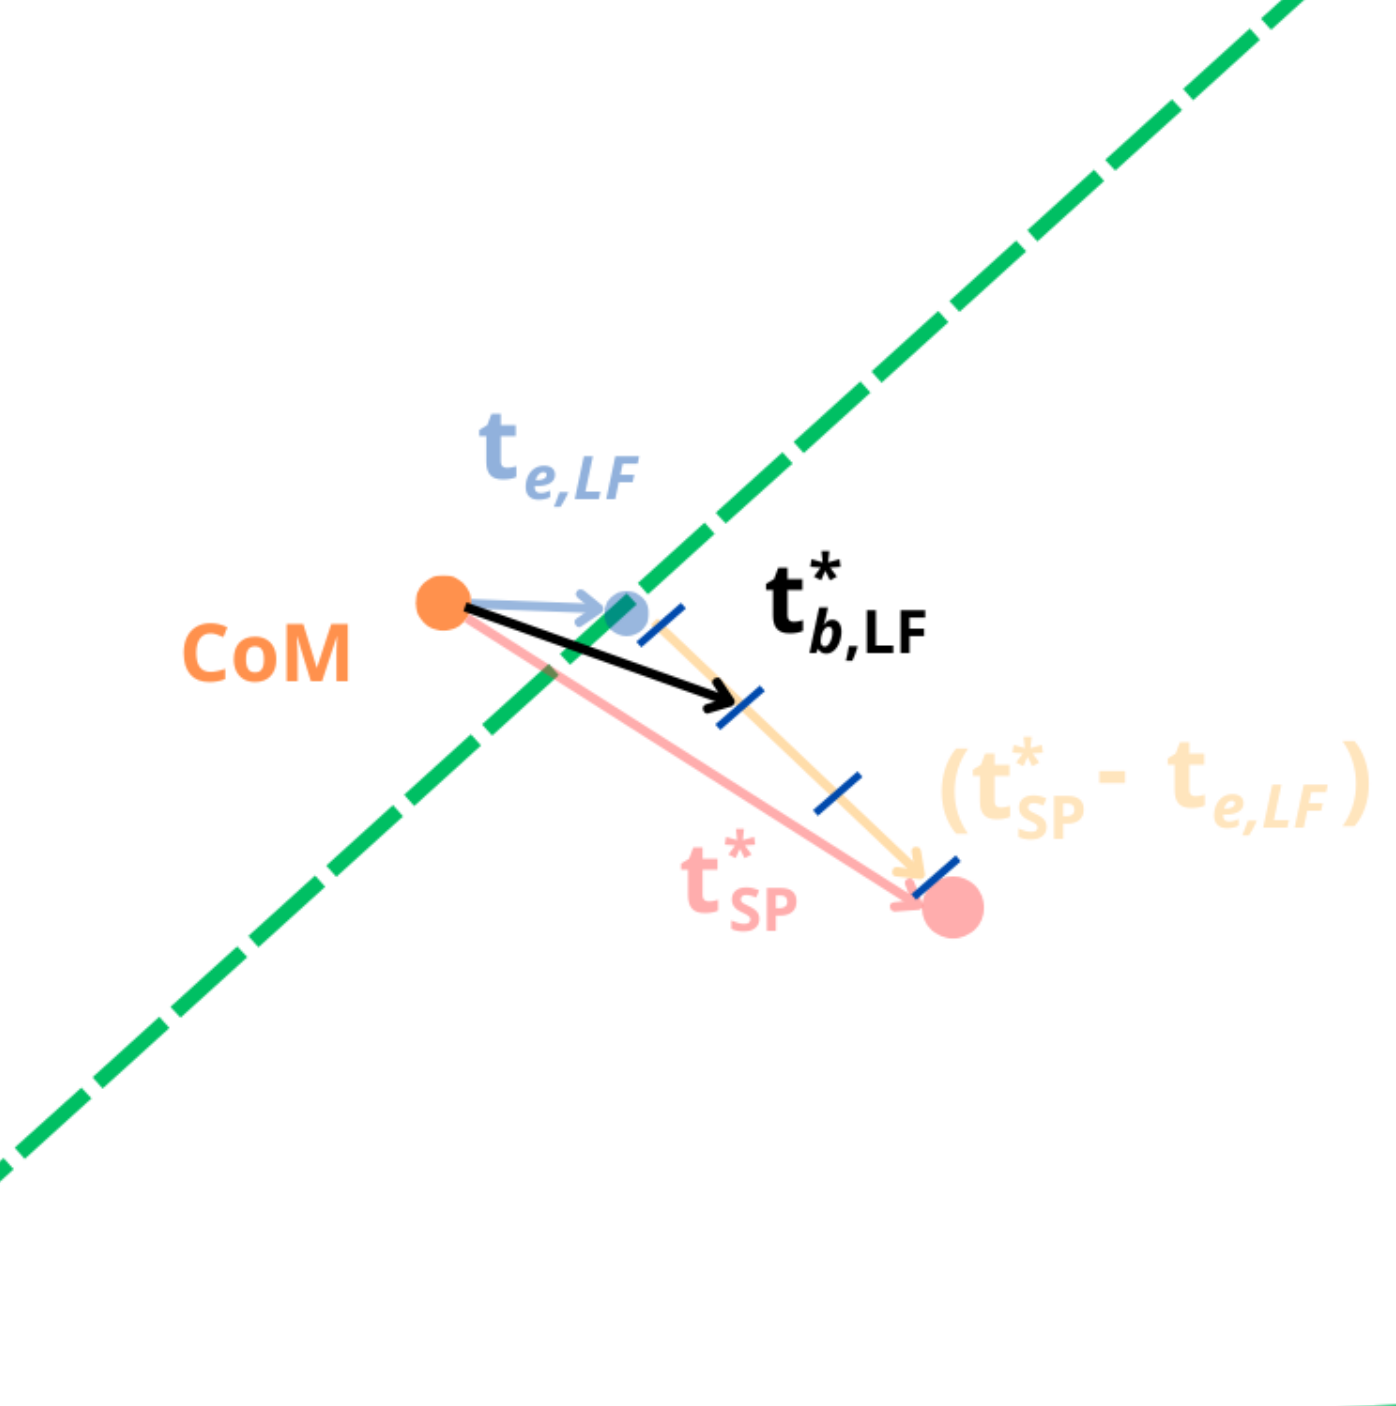
\includegraphics[width=0.3\textwidth]{Images/img_ch5/translation3_ex1.png}}   \quad
    \\
    \subfloat[$j=RF$,Upcoming support polygon\label{fig:translation1_ex2}]{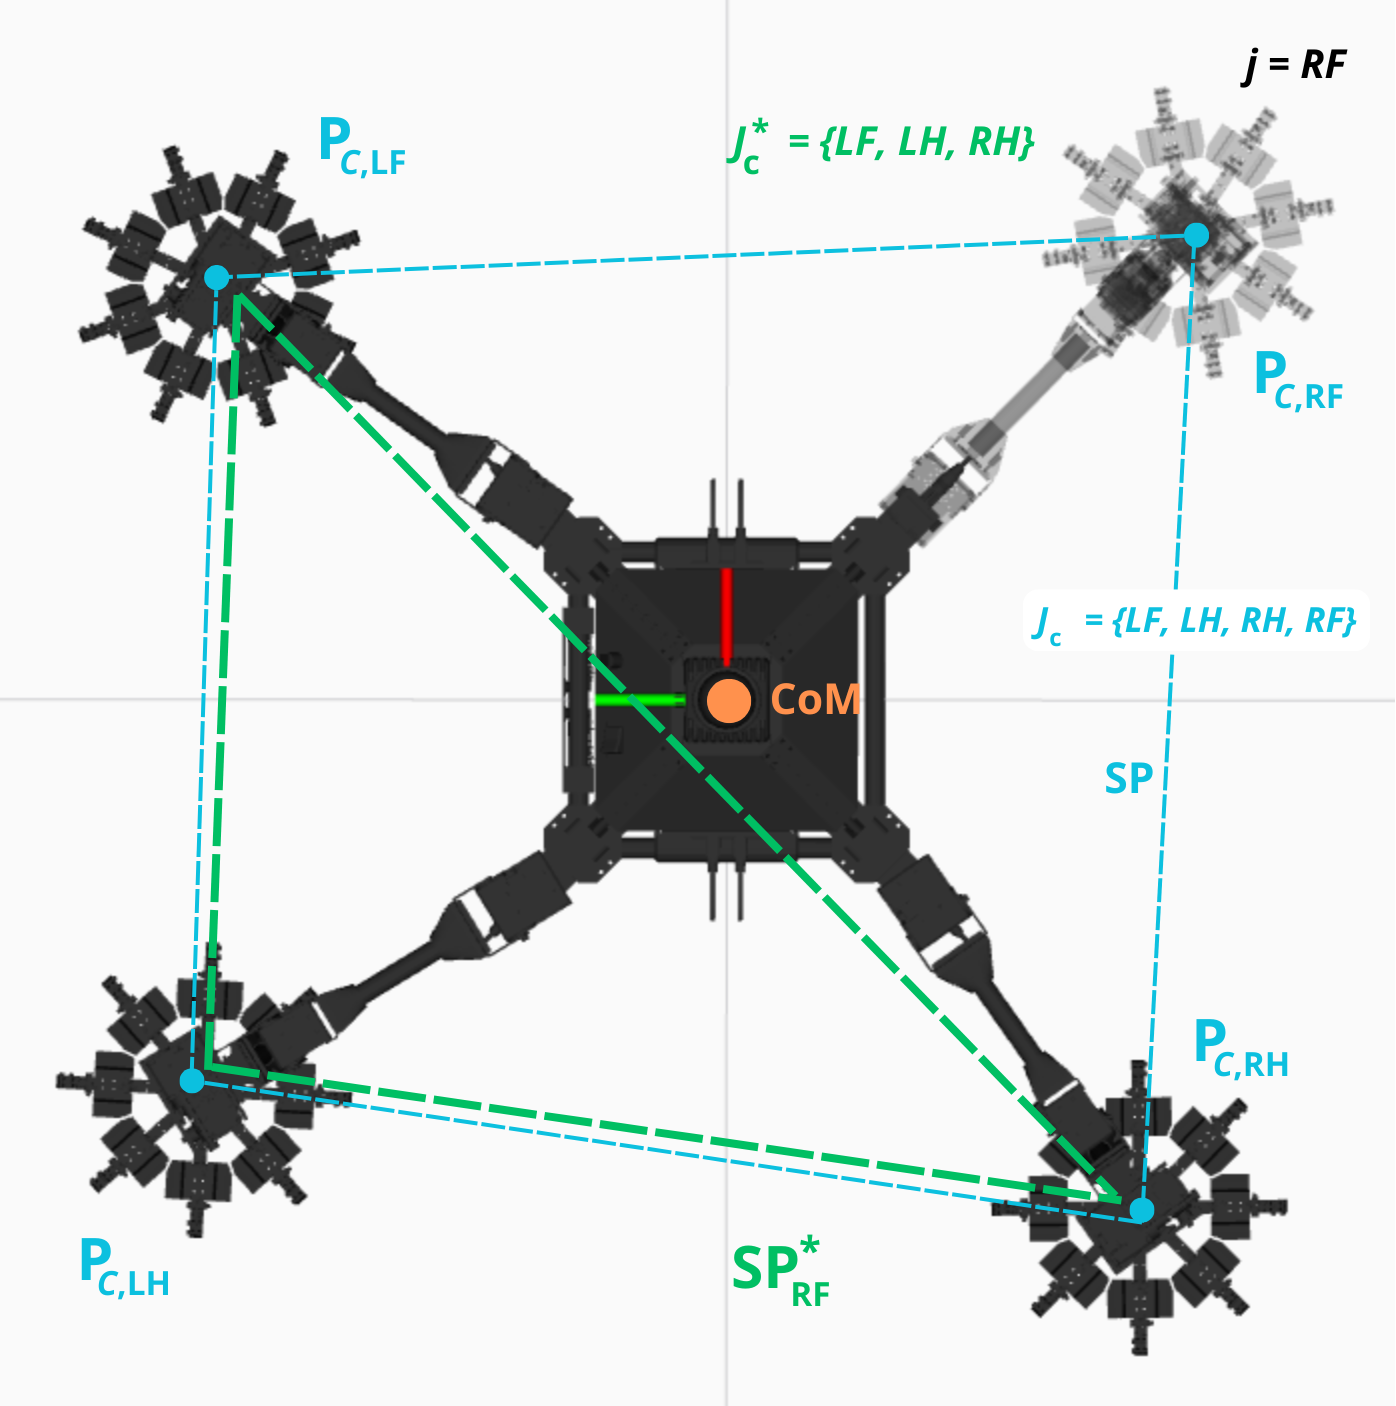
\includegraphics[width=0.3\textwidth]{Images/img_ch5/translation1_ex2.png}}\quad
    \subfloat[Involved vectors\label{fig:translation2_ex2}]{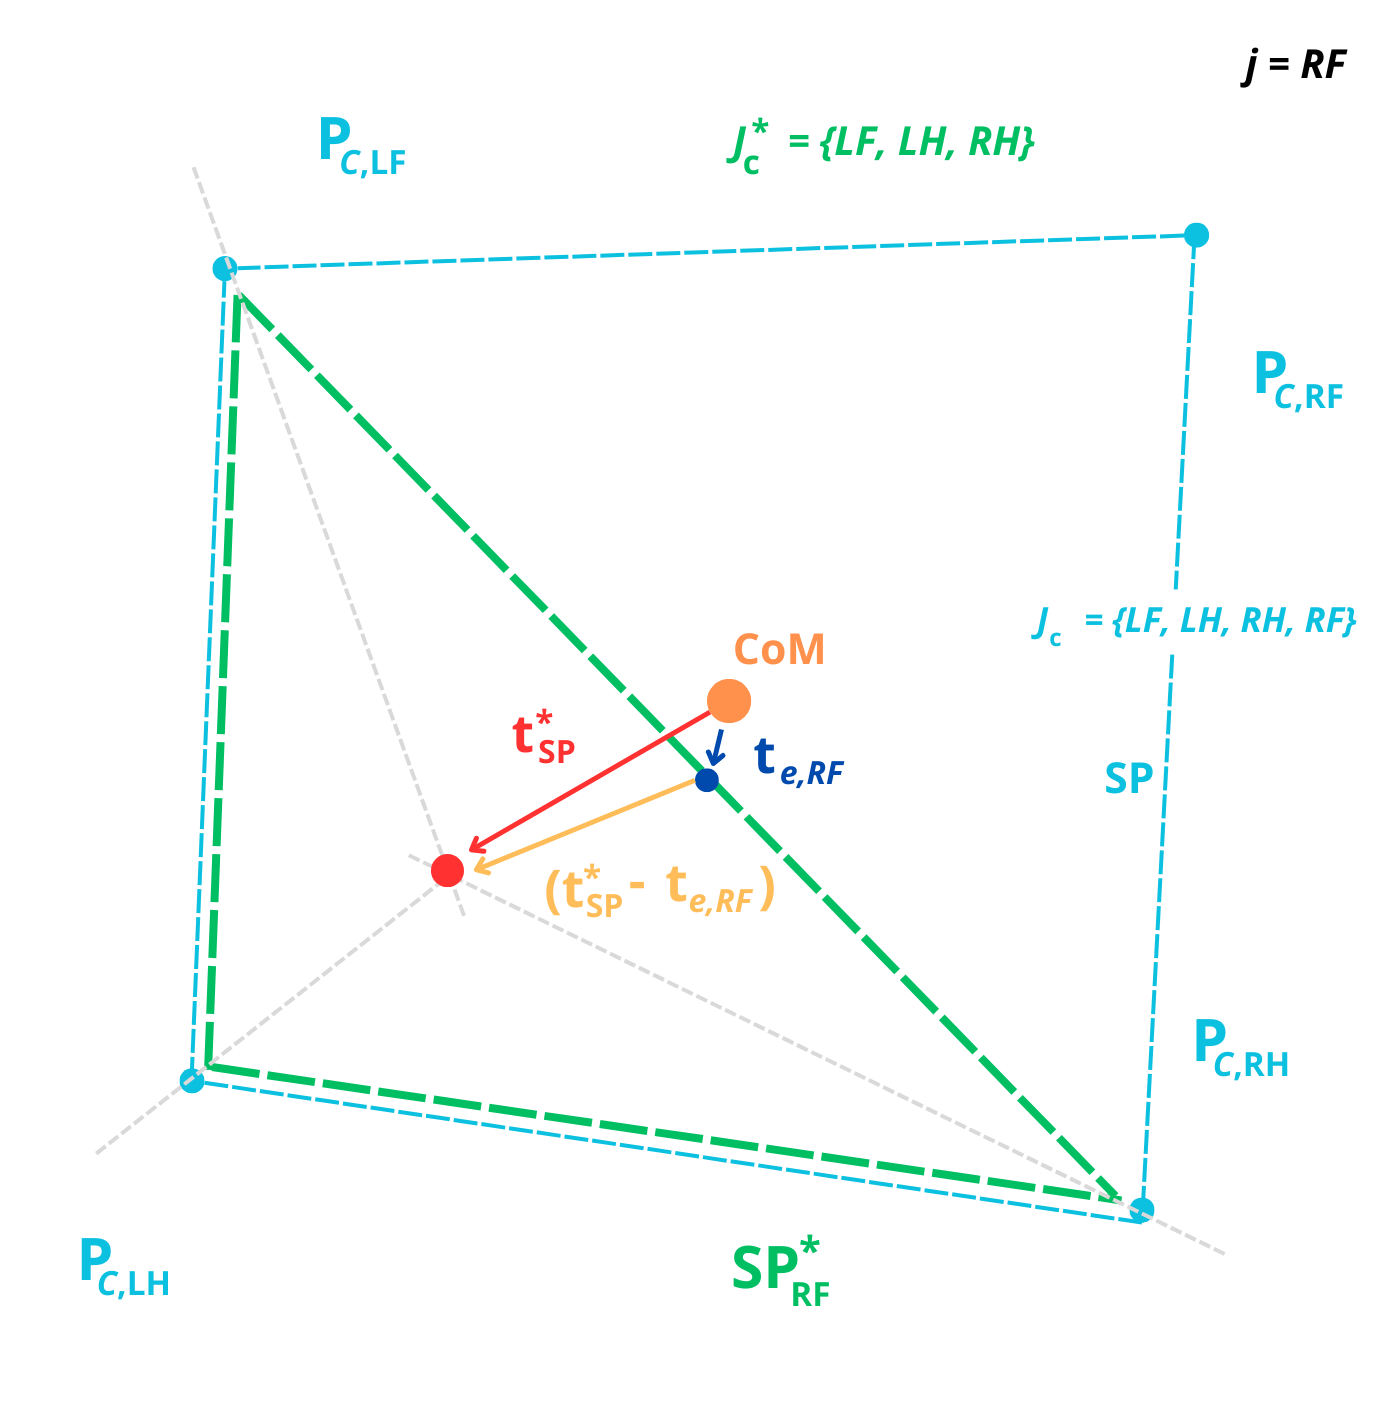
\includegraphics[width=0.3\textwidth]{Images/img_ch5/translation2_ex2.png}}\quad
    \subfloat[Final base translation\label{fig:translation3_ex2}]{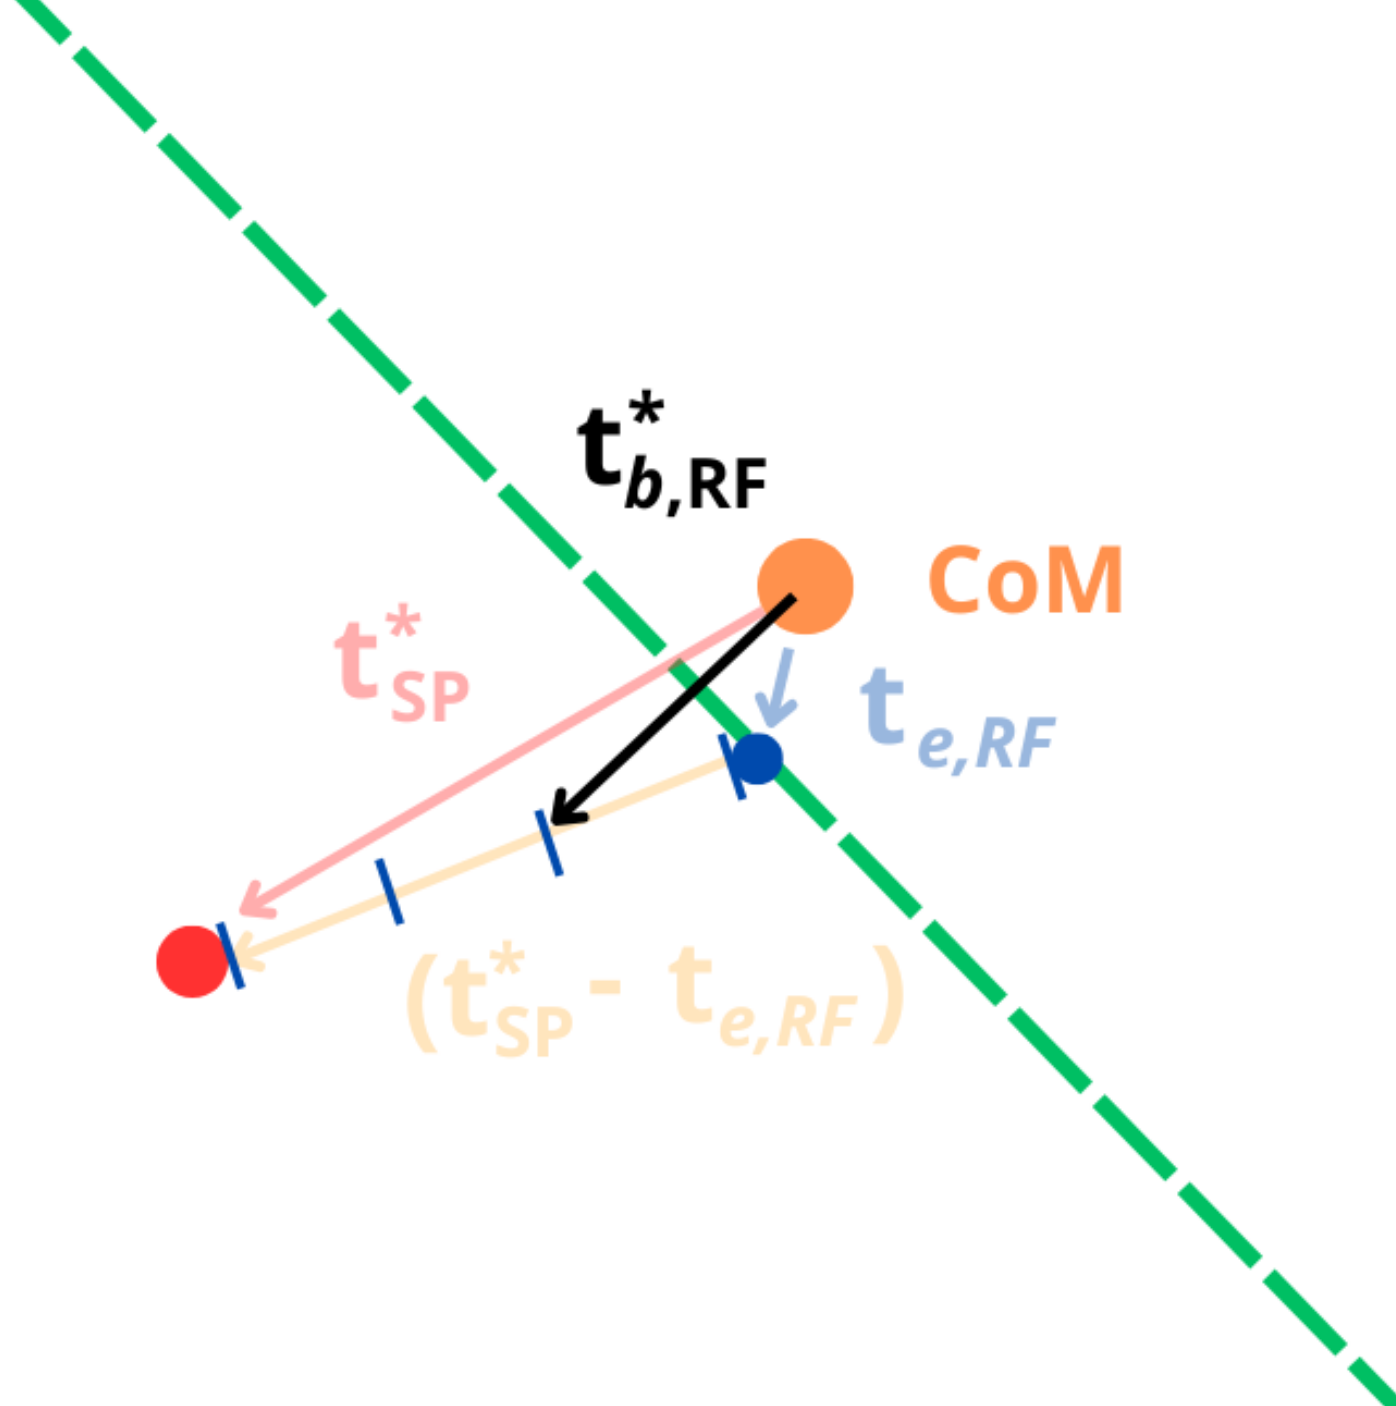
\includegraphics[width=0.3\textwidth]{Images/img_ch5/translation3_ex2.png}}
    \caption[Schematic representation of base translation rule of thumb]{Schematic representation of base translation rule of thumb}
    \label{fig:base_rule_of_thumb}
\end{figure}

The rule of thumb used to position the base of LIMBERO-GRIEEL is schematized for different SP cases in Fig.\ref{fig:base_rule_of_thumb} above, and can be formalized mathematically. Considering all the vectors measured in a frame attached to $\overline{\mathbf{P}_{CoM}}$, and denoting with $\mathbf{t^*_b}_{,j}$ the required base motion when limb $j$ is the upcoming rising limb, $\mathbf{t^*_{SP}}$ the upcoming SP center, and $\mathbf{t_e}_{,j}$ the midpoint of the edge connecting the adjacent limbs (for example, the adjacent limbs of LF are LH and RF, while RH is the opposite), the base motion is computed as:   
\begin{equation}
    \label{eq:base_motion_rule_of_thumb}
    \mathbf{t^*_b}_{,j} = \mathbf{t_e}_{,j} +  \frac{(\mathbf{t^*_{SP}} - \mathbf{t_e}_{,j})}{3} 
\end{equation}
Simplified to 
\begin{equation}
    \label{eq:base_motion_rule_of_thumb_final}
    \mathbf{t^*_b}_{,j} = \frac{2}{3}\mathbf{t_e}_{,j} + \frac{1}{3}\mathbf{t^*_{SP}} 
\end{equation}

Denoting with $SP_j^*$ the upcoming support pattern ($SP^* \subset SP$) when limb $j$ is raised and all $k\not=j$ limbs' contact points $\mathbf{P}_{c,k}$ fixed, and with $J_c^* = J_c/j$ the upcoming set of contact points. Considering that before the transformation, if all limbs are in contact (included as an initial condition) $J_c = J$, it holds: 
\begin{equation}
    \label{eq:upcoming_SP}
    SP^* = Conv(J_c^*) 
\end{equation}
Where $Conv(\cdot)$ denotes the convex hull as defined in (\ref{eq:SP}).

In Equation \ref{eq:base_motion_rule_of_thumb} the meaning of that base translation is clear:\\
the final base position is such that the CoM will project in a point which is at $\frac{1}{3}$ of the length of the segment between the midpoint of the closest $SP^*$ edge and the center of $SP^*$. \\
So, in any condition, it holds $SSM^* = \frac{1}{3}max(SSM)$.

It is possible to compute $\mathbf{t^*_{SP}}$ and $\mathbf{t_e}_{,j}$ as:
\begin{equation}
    \label{eq:SP_center}
    \mathbf{t^*_{SP}} = \frac{\sum_{k\in J^*_c}\mathbf{P}_{c,k}}{3}
\end{equation}
\begin{equation}
    \label{eq:middle_vec}
    \mathbf{t_e}_{,j} = 
    \begin{cases}
    \frac{\mathbf{P}_{c,LF} + \mathbf{P}_{c,RH} }{2} \quad if \text{ } j\in \{LH,RF\}
    \\
    \frac{\mathbf{P}_{c,RF} + \mathbf{P}_{c,LH} }{2} \quad if \text{ } j \in \{LF,RH\}
    \end{cases}
\end{equation}

The definition of the $SP$ and $SP^*$ is fundamental to understanding the theory, but in principle, to compute the desired base translation, the set of contact points $\mathbf{P_c} = \{\mathbf{P}_{c,j} | j\in J_c\}$ is enough. 

So, based on equations (\ref{eq:base_motion_rule_of_thumb_final})(\ref{eq:SP_center})(\ref{eq:middle_vec}) it is possible to define a primitive procedure, that returns the desired base translation given the set of contact points and the limb to raise:
\begin{equation*}
    \textit{BaseTranslation}^*: (\mathbf{{P}_c}, j) \rightarrow \mathbf{t^*_b}_{,j}
\end{equation*}

Finally, all the elements to define the motion sequence for a single are formalized, and the complete procedure is formalized in  (\ref{alg:single_grieel_transition}), with the proper level of detail.
This computational sequence corresponds to the steps previously defined.
The details on limb height, wrist configuration, and grieel mode are neglected here, but implemented in the final software. A schematic representation of this together with the real system sequence is reported in Fig.\ref{fig:single_limb_transform}.

\begin{algorithm}[H]

    \caption{SingleGRIEEL\_Transformation($\mathbf{P_c}$, $j$)}
    \label{alg:single_grieel_transition}
    \begin{algorithmic}[1]
    \IF{$|\mathbf{P_c}| < 4$}
    \STATE{\textbf{return} FAIL "Not enough limbs in contact"}
    \ENDIF
    \STATE{$\mathbf{t^*_b}_{,j} \leftarrow \textit{BaseTranslation}^*$($\mathbf{P_c}$, $j$)}
    \STATE{Move the base by $\mathbf{t^*_b}_{,j}$ (base motion task)}
    \WHILE{base task \textbf{not} finsh}
    \STATE{check and wait}
    \ENDWHILE
    \STATE{Raise limb $j$ (limb motion task)}
    \WHILE{limb task \textbf{not} finish}
    \STATE{check and wait}
    \ENDWHILE
    \STATE{Send new joint set point $j\_wristH$, $j\_wristV$}
    \STATE{Send new open/closing command (GRIEEL change task)}
    \WHILE{grieel task \textbf{not} finish}
    \STATE{check and wait}
    \ENDWHILE
    \STATE{lay down limb $j$ (limb motion task)}  
    \STATE{\textbf{return} SUCCESS} 
    \end{algorithmic}
\end{algorithm} 


\begin{figure}[H]
    \centering
    \subfloat[Compute base translation\label{fig:single_1}]{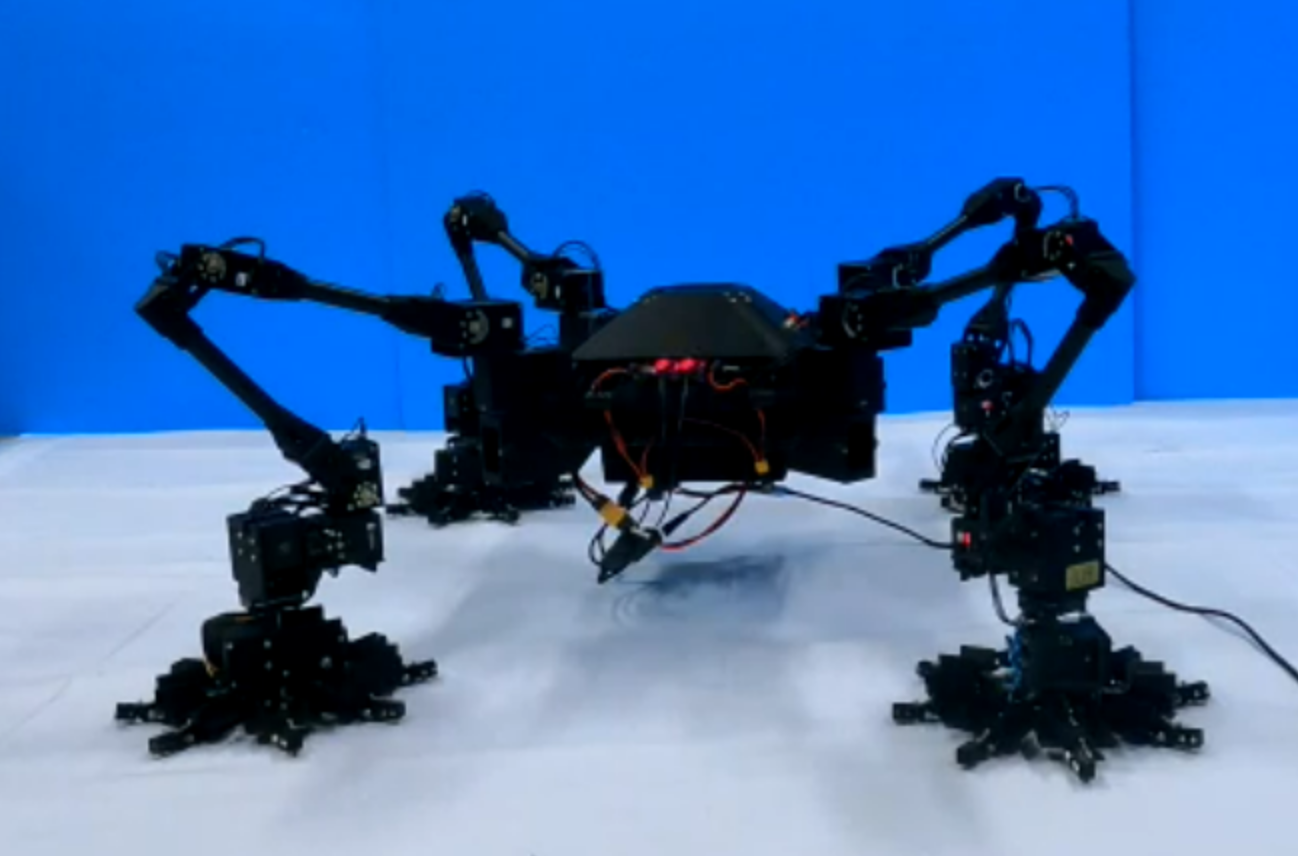
\includegraphics[width=0.3\textwidth]{Images/img_ch5/robot_G2W_1.png}} \quad 
    \subfloat[Move the base\label{fig:single_2}]{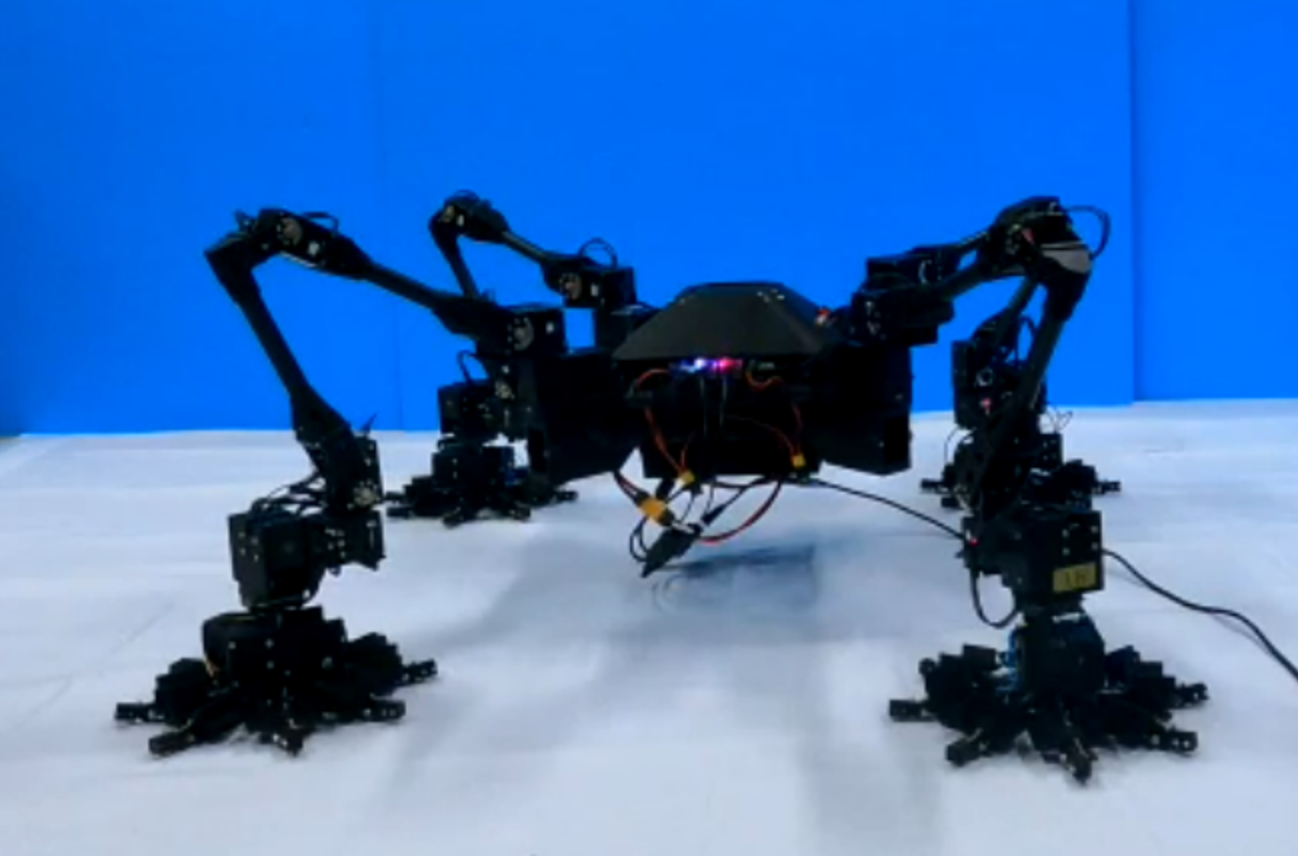
\includegraphics[width=0.3\textwidth]{Images/img_ch5/robot_G2W_2.png}} \quad
    \subfloat[Raise the limb\label{fig:single_3}]{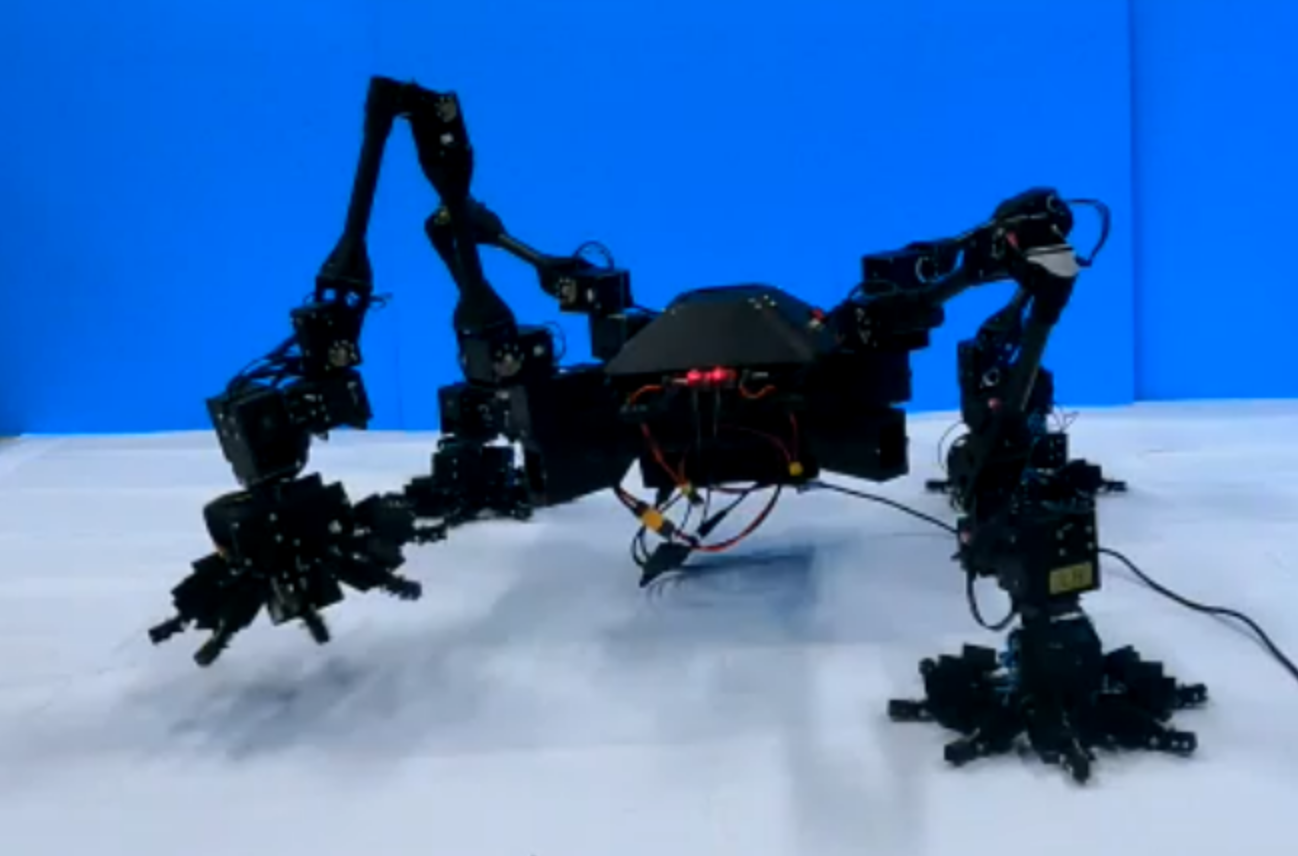
\includegraphics[width=0.3\textwidth]{Images/img_ch5/robot_G2W_3.png}}   \quad
    \\
    \subfloat[Change wrist joints\label{fig:single_4}]{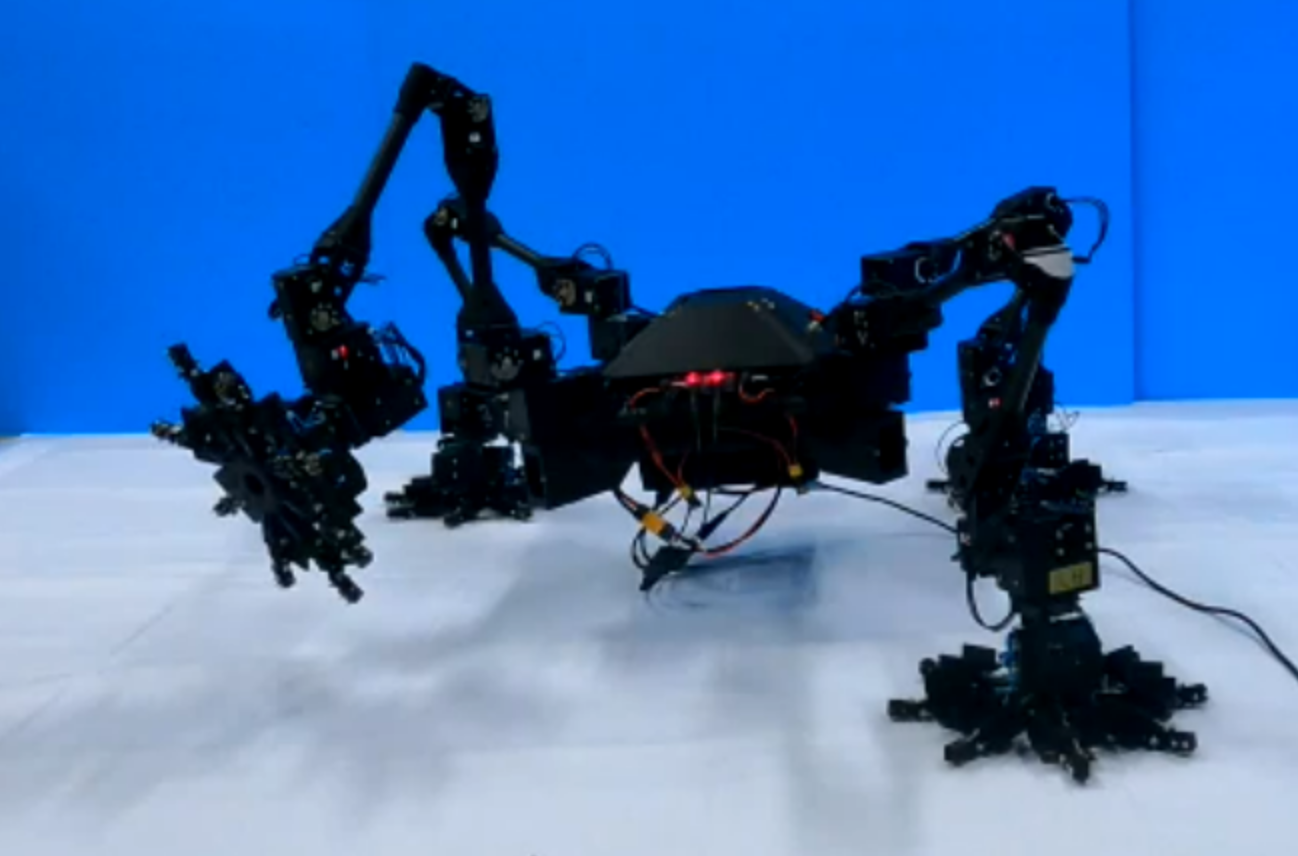
\includegraphics[width=0.3\textwidth]{Images/img_ch5/robot_G2W_4.png}}\quad
    \subfloat[Transform GRIEEL \label{fig:single_5}]{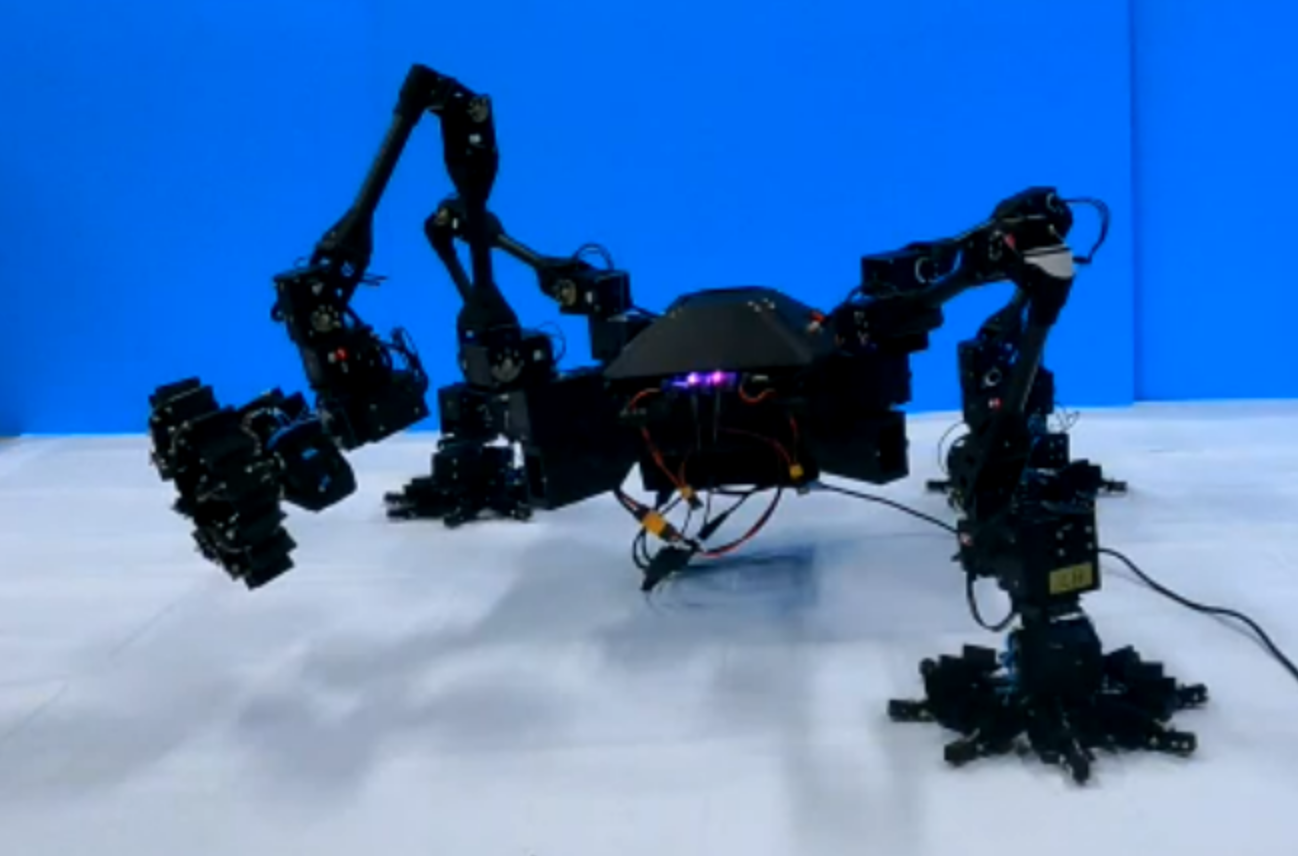
\includegraphics[width=0.3\textwidth]{Images/img_ch5/robot_G2W_5.png}}\quad
    \subfloat[Lay down the limb\label{fig:single_6}]{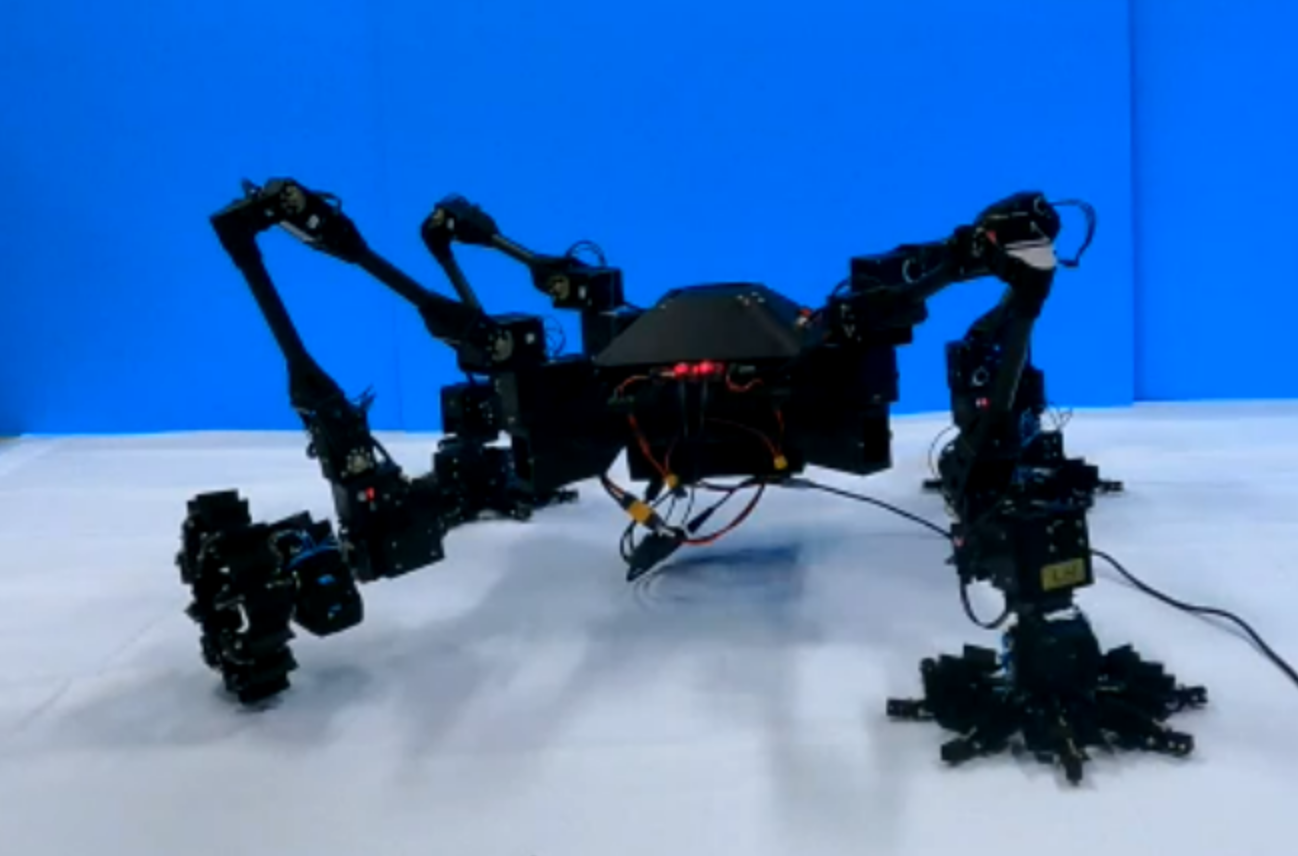
\includegraphics[width=0.3\textwidth]{Images/img_ch5/robot_G2W_6.png}}
    \caption[Single limb transition sequence]{Single limb transition sequence}
    \label{fig:single_limb_transform}
\end{figure}

Then, exploiting the procedure defined above, a full locomotion transition is easy to define as a special case of multiple limb transition, where $J^* = J$, with $J^*$ as the ordered set of limbs to transform. Before defining it, an additional primitive procedure that returns the set of contact point positions is needed (on software, managed by state estimators):
\begin{equation*}
    \textit{CheckContact}: () \rightarrow \mathbf{P_c}
\end{equation*}
Finally, all the required elements are defined, the algorithm is reported below, and Fig.\ref{fig:complete_transition} summarizes it with a simple high-level diagram. 

\begin{algorithm}[H]
    \caption{MultipleGRIEEL\_Transformation($\mathbf{P_c}$, $J^*$)}
    \label{alg:multiple_grieel_transition}
    \begin{algorithmic}[1]
    \STATE{$N_{task} \leftarrow |J^*|$}
    \STATE{$first\_limb \leftarrow$ True}
    \STATE{$finish\_transform \leftarrow$ False}
    \IF{$|\mathbf{P_c}| < 4$}
    \STATE{\textbf{return} FAIL "Not enough limbs in contact"}
    \ENDIF
    \FOR{$l = 1,...,N_{task}$}
    \IF{$(first\_limb \textbf{ or } finish\_transform)$}
    \STATE{$\mathbf{P_c} \leftarrow \textit{CheckContact}$}
    \STATE{$\textit{result} \leftarrow SingleGRIEEL\_Transformation$ ($\mathbf{P_c}$, $l$)}
    \IF{$result = SUCCESS$}
        \STATE{$finish\_transform \leftarrow$ True} 
    \ELSE
        \STATE{\textbf{return} FAIL "Error during limb $l$ Transformation"}
    \ENDIF
    \ENDIF
    \ENDFOR
    \STATE{\textbf{return} SUCCESS} 
    \end{algorithmic}
\end{algorithm} 

\begin{figure}[H]
    \centering
    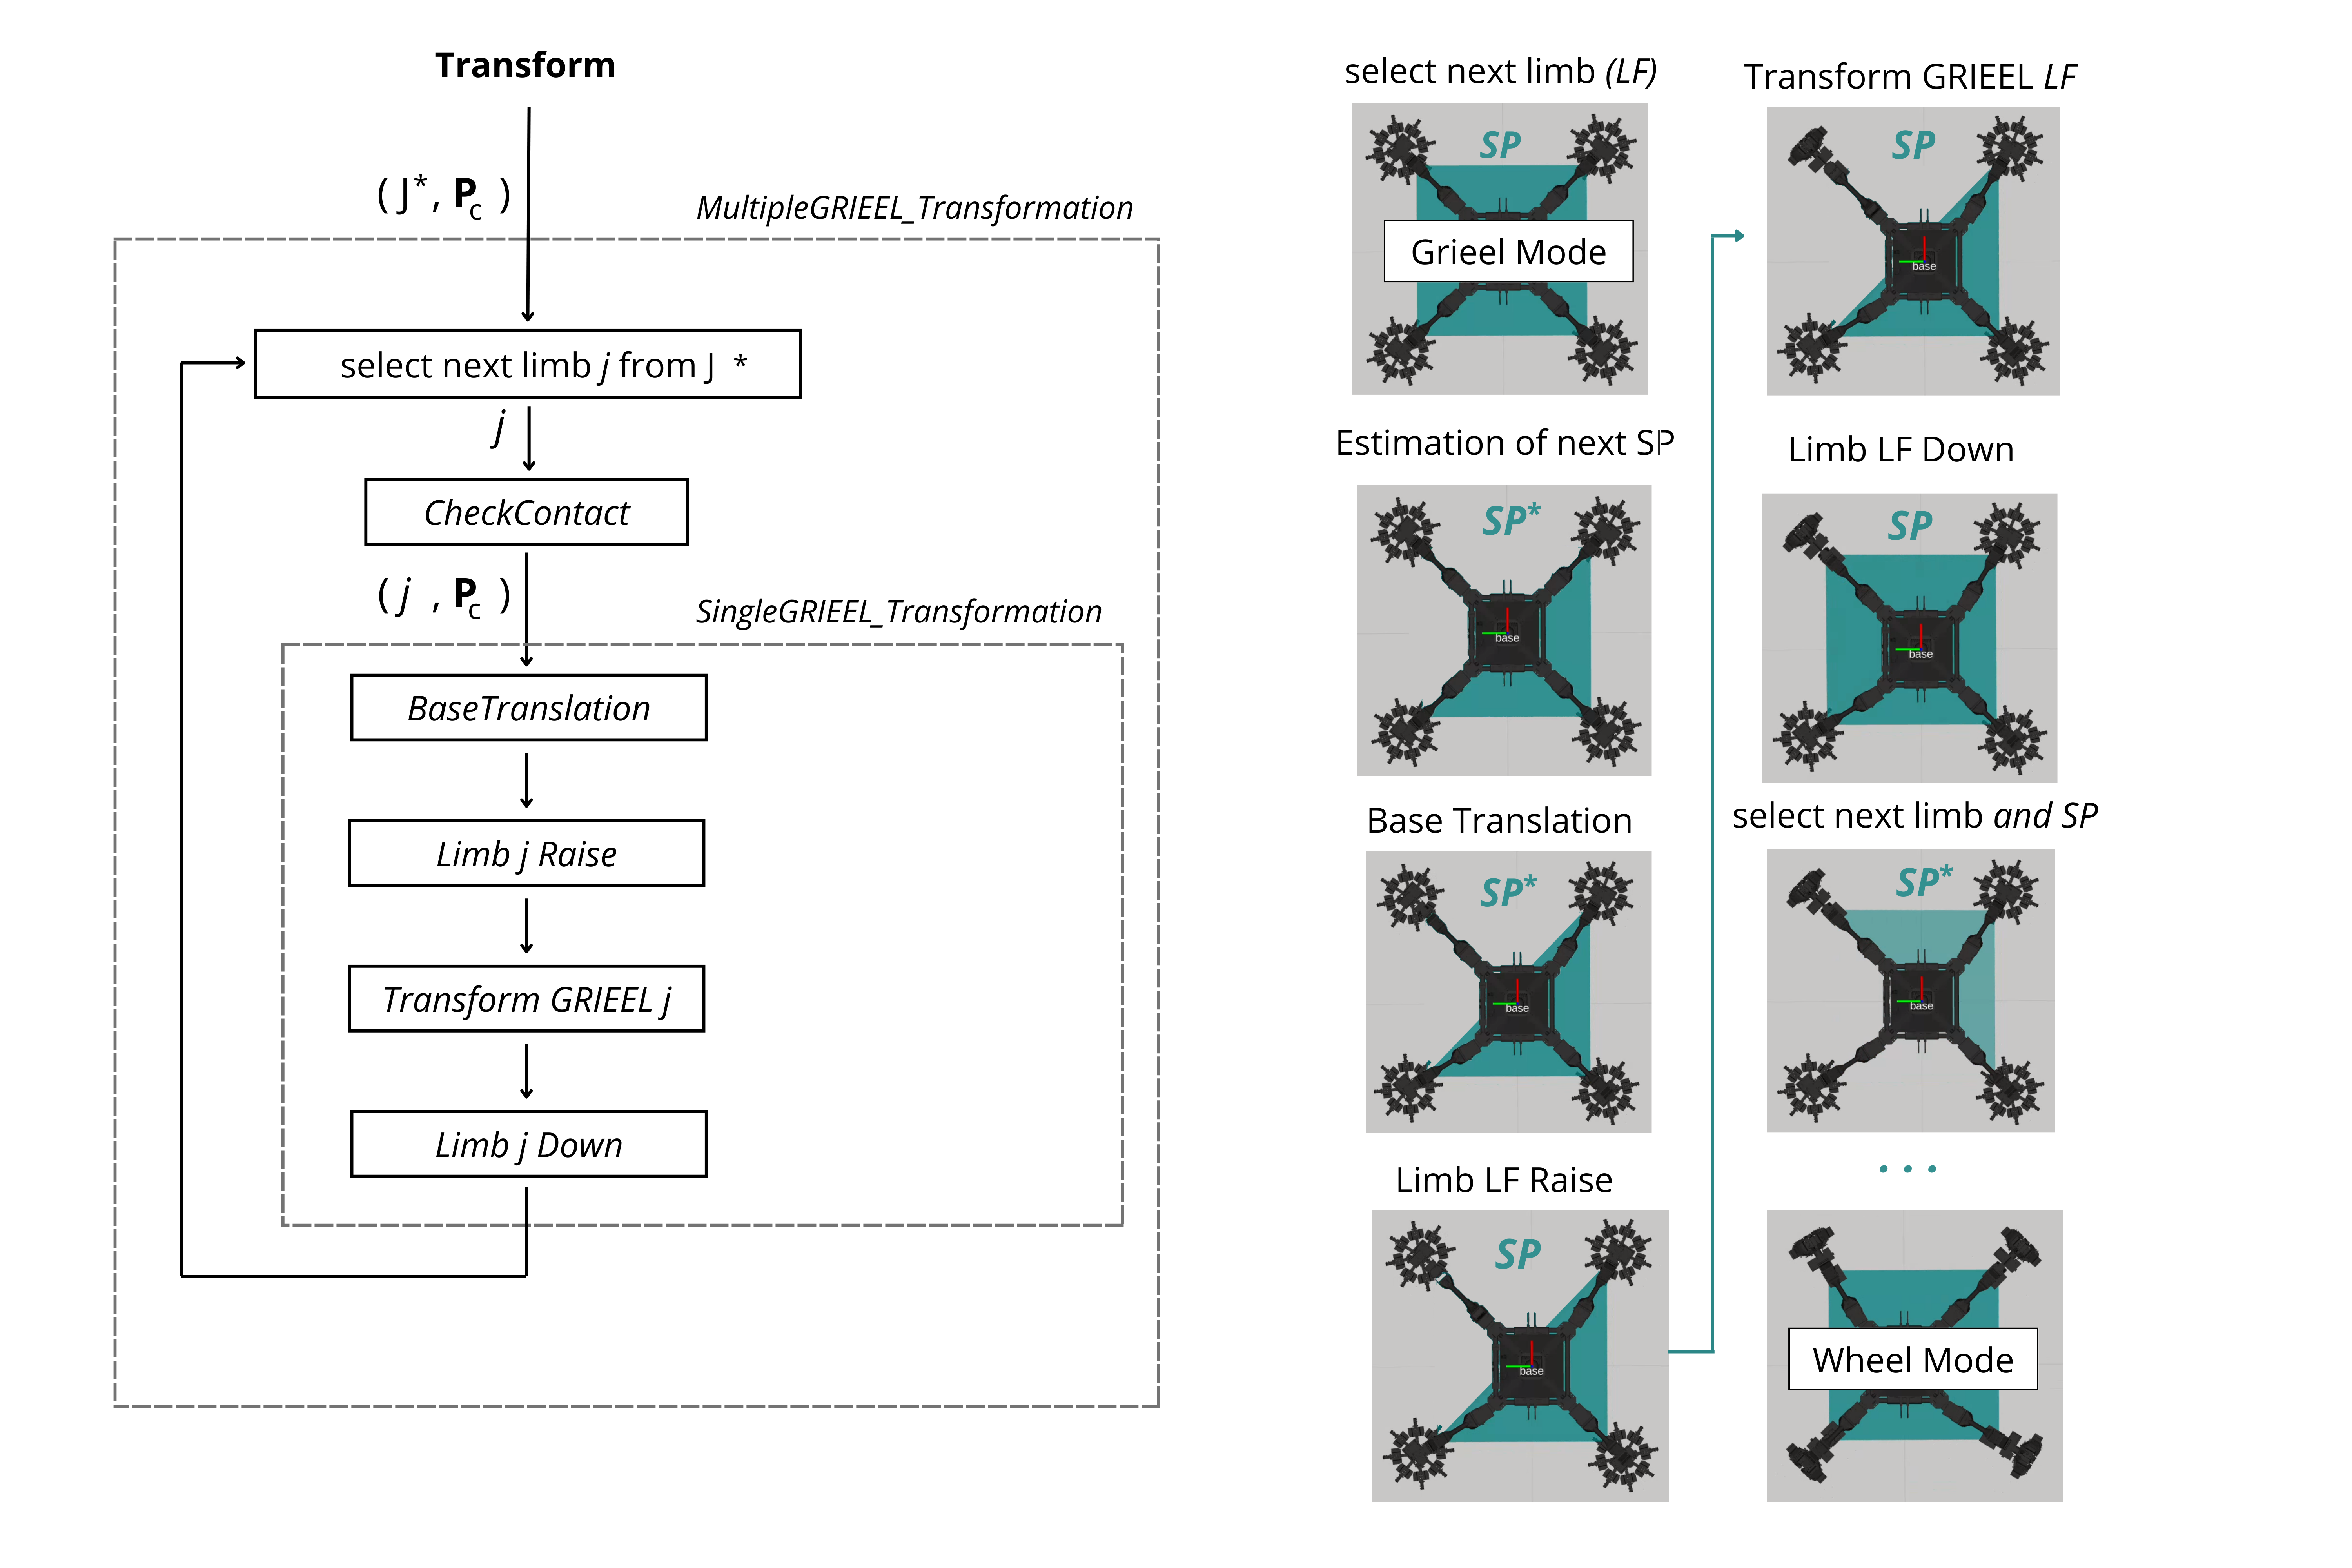
\includegraphics[width=1.1\textwidth]{Images/img_ch5/complete_transition.png}
    \caption{Schematic representation of the transformation algorithm}
    \label{fig:complete_transition}
\end{figure}


\section{Manipulability analysis with ATBVME and SSM}
\label{sec:base_ellipsoid_algorithm}

In the previous section, the autonomous and adaptable transformation algorithm has been formally defined and qualitatively analyzed. From that description, it can be identified as an anticipative planner, computing motion tasks based on the future robot configuration estimation, with the objective of optimizing stability and dexterity. 
The quantification of these performance requirements is now addressed with a kinematic analysis, using the ATBVME for dexterity and the SSM for stability. 

Furthermore, to derive a more general performance measure, a normalized percentage SSM has been defined as: 

\begin{equation}
    \label{eq:base_motion_rule_of_thumb_final}
    SSM_\% = \frac{SSM}{SSM_{max}}\cdot100
\end{equation}

With the SSM defined in Eq.\ref{eq:SSM_2} (considered null if negative), and the $SSM_{max}$ as maximum stability margin when all four limbs touch the ground in the standard walking configuration (reported in Fig.\ref{fig:limbero_walking}). 
This normalized index is useful to compare different multilimbed robotic systems, defining a measure independent from the robot dimension.  

The algorithm has been implemented in MATLAB with the DH kinematic model derived from the URDF description, and the results of some steps of a gripper-to-wheel transformation sequence are reported in Fig.\ref{fig:G2W_analysis_LF} and \ref{fig:G2W_analysis_RF} below. The transition sequence has been tested with $J^* = \{LF, LH, RH, RF\}$. The graphical elements are interpreted as defined in Chapter \ref{sec:ME_multi_limb_example}, with the additional \textbf{Upcoming Support Polygon}, identified by a blue discontinuous line perimeter, and the end effector represented by a red circle (Wheel or Gripper). 

The rule of thumb defined previously ensures a $SSM_{max}$ always above the $15\%$, and an ATBVME with preferred direction of motion parallel to the ground plane, in the base xy plane(cutting the ellipsoid with a plane on the xy plane o the base frame, it is a circle). This dexterity property ensures ease of base translation in the xy plane, and in case of unexpected disturbances, it guarantees a quick and effective response for base stabilization. 

Now, the performance above is compared with the redefined sequence, where the base motion task is computed maximizing the SSM on three contact limbs (moving in the upcoming support center): 
\begin{equation}
    \label{eq:base_motion_rule_centering}
    \mathbf{t^*_b}_{,j} = \mathbf{t^*_{SP}}
\end{equation}

With this redefinition, only stability is considered, and the results are reported in Fig.\ref{fig:G2W_optimal_analysis_LF} and \ref{fig:G2W_optimal_analysis_RF}. The increase in stability is proven by the fact that the $SSM_\%$ is maintained above 45\% during the transition. However, higher base displacements are involved in reaching the configuration with maximum stability.  
Comparing the ATBVME (as in Fig.\ref{fig:base_LF} and Fig.\ref{fig:base_LF_opt}, or Fig.\ref{fig:base_RF} and Fig.\ref{fig:base_RF_opt}), when the base task is computed as in (\ref{eq:base_motion_rule_centering}), the preferred direction of motion has a non-negligible rotation from the xy plane.

As discussed in Chapter\ref{ch:chapter_three}, the direction of the ellipsoid major axis is the relevant information to analyze dexterity, meaning that, the rotated ellipsoid is interpreted as a dexterity loss in the main direction of base stabilization. In conclusion, the rule of thumb is optimal in terms of manipulability, if stability is important, the next support center can be integrated in the transformation sequence.

Finally, the driving configuration after G2W transition is reported in Fig.\ref{fig:Driving_Manipulability}.

\begin{figure}[H]
    \centering
    \subfloat[Next support polygon estimation\label{fig:support_LF}]{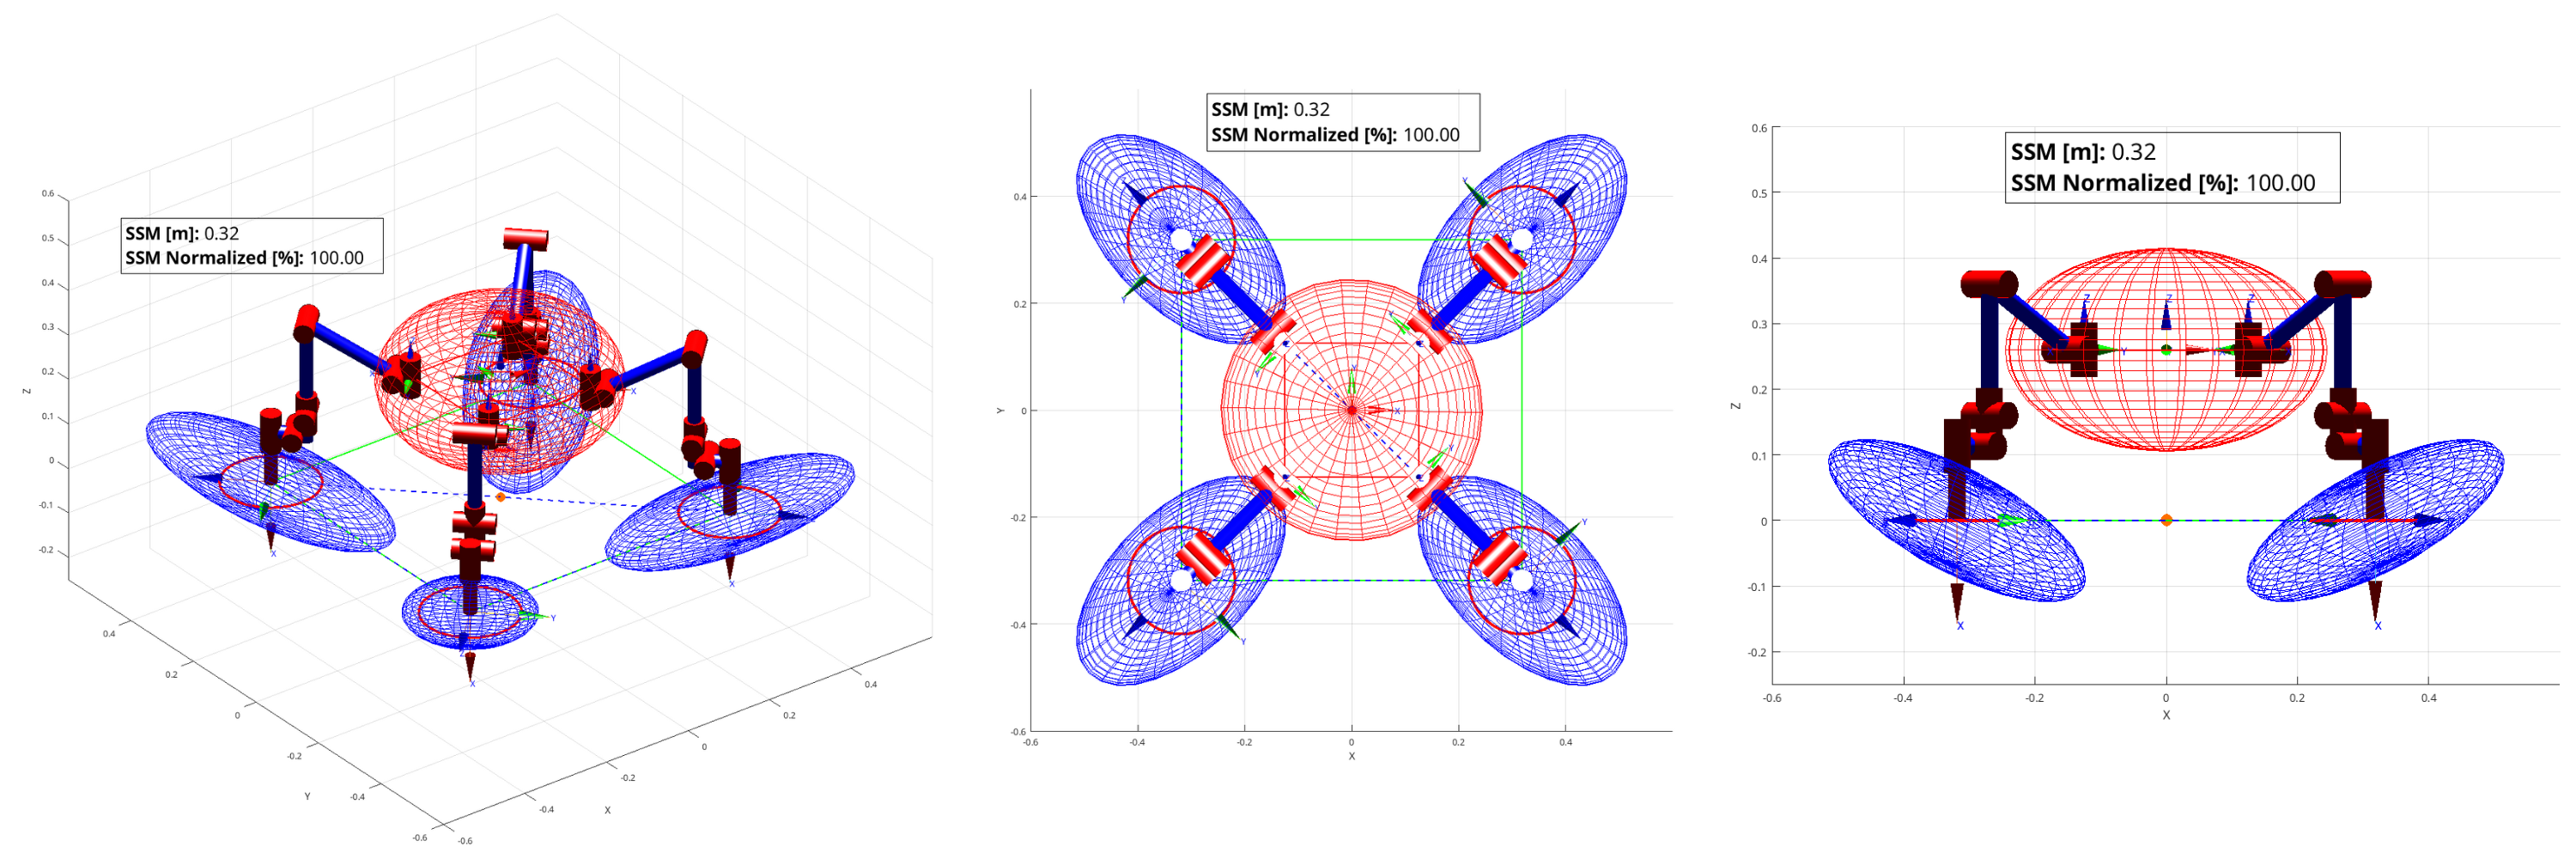
\includegraphics[width=0.9\textwidth]{Images/img_ch5/step1_ruleofthumb.png}} 
    \\
    \subfloat[Base motion task\label{fig:base_LF}]{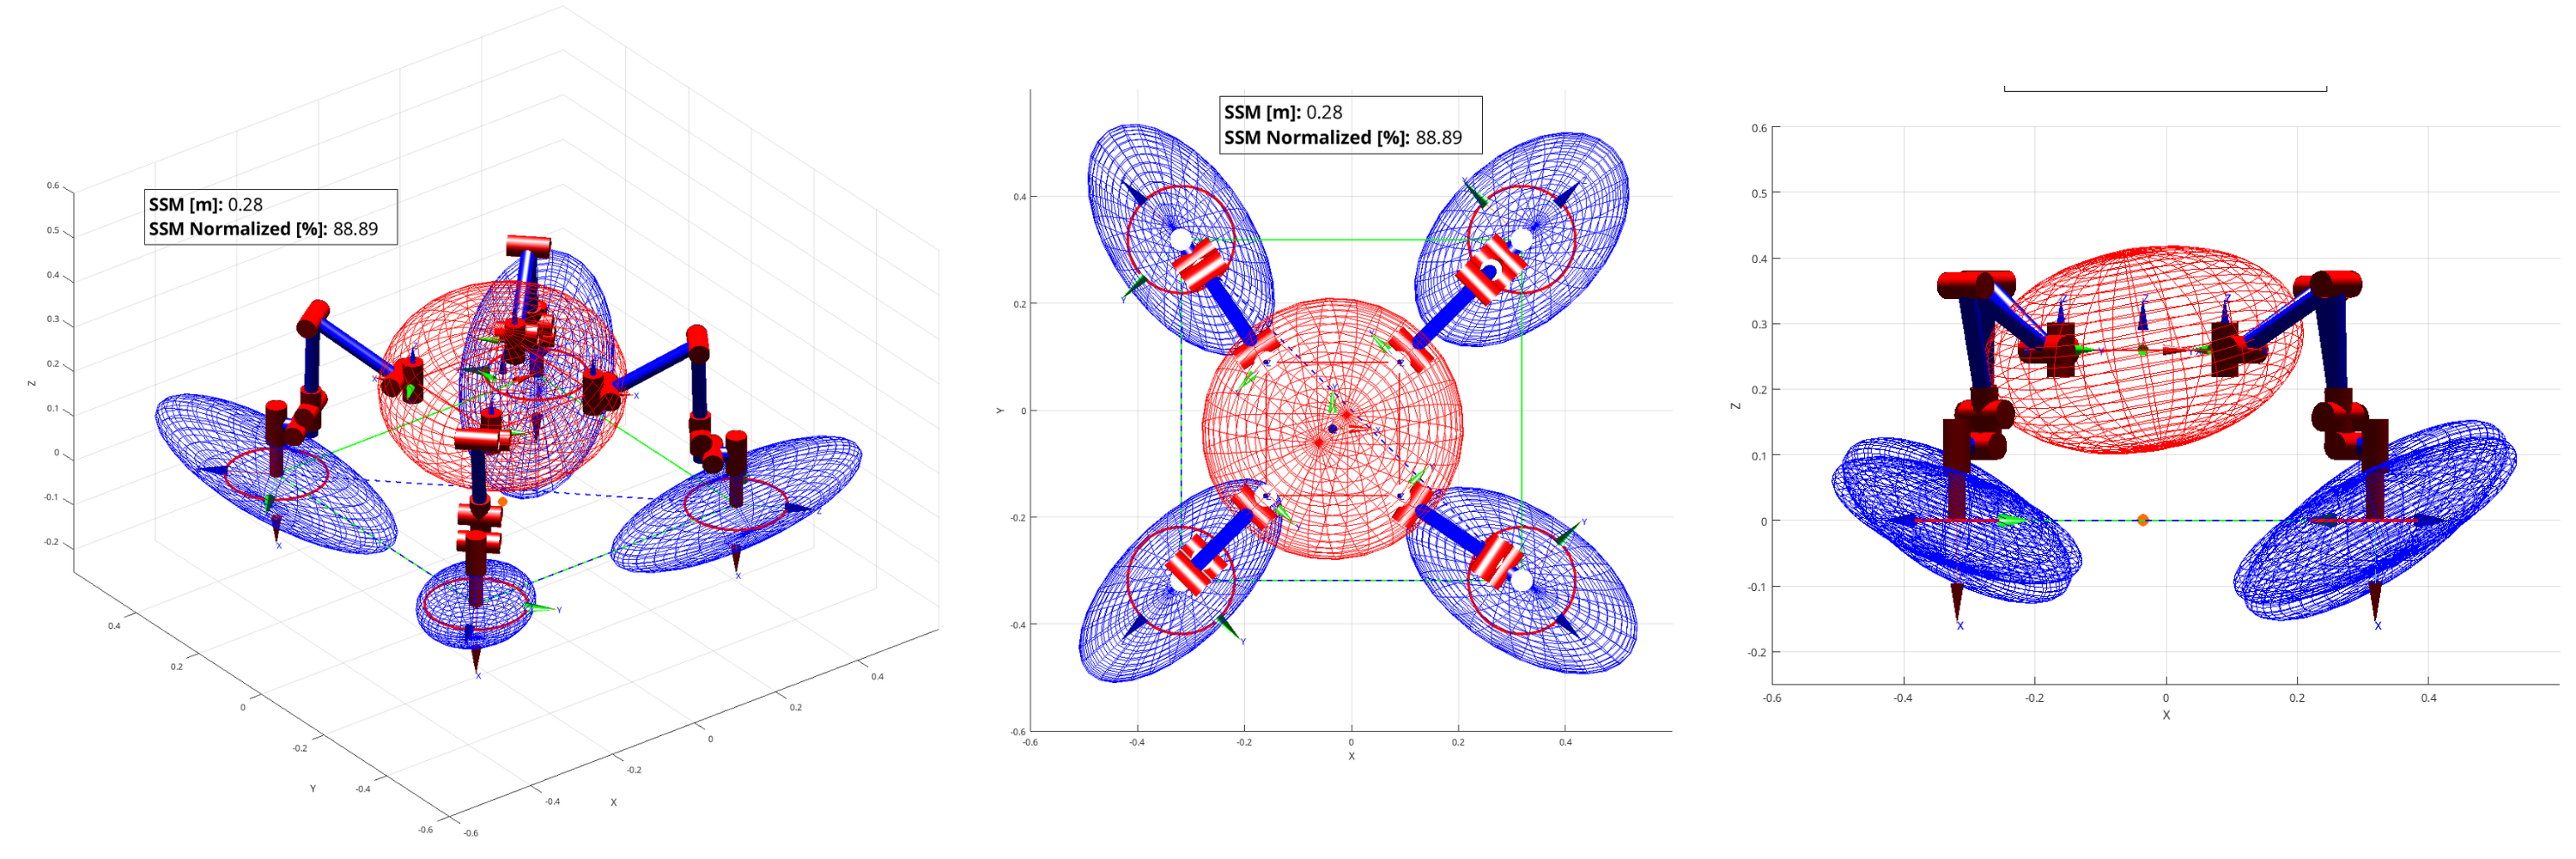
\includegraphics[width=0.9\textwidth]{Images/img_ch5/step2_ruleofthumb.png}} 
    \\
    \subfloat[Raise limb and GRIEEL transformation\label{fig:raise_LF}]{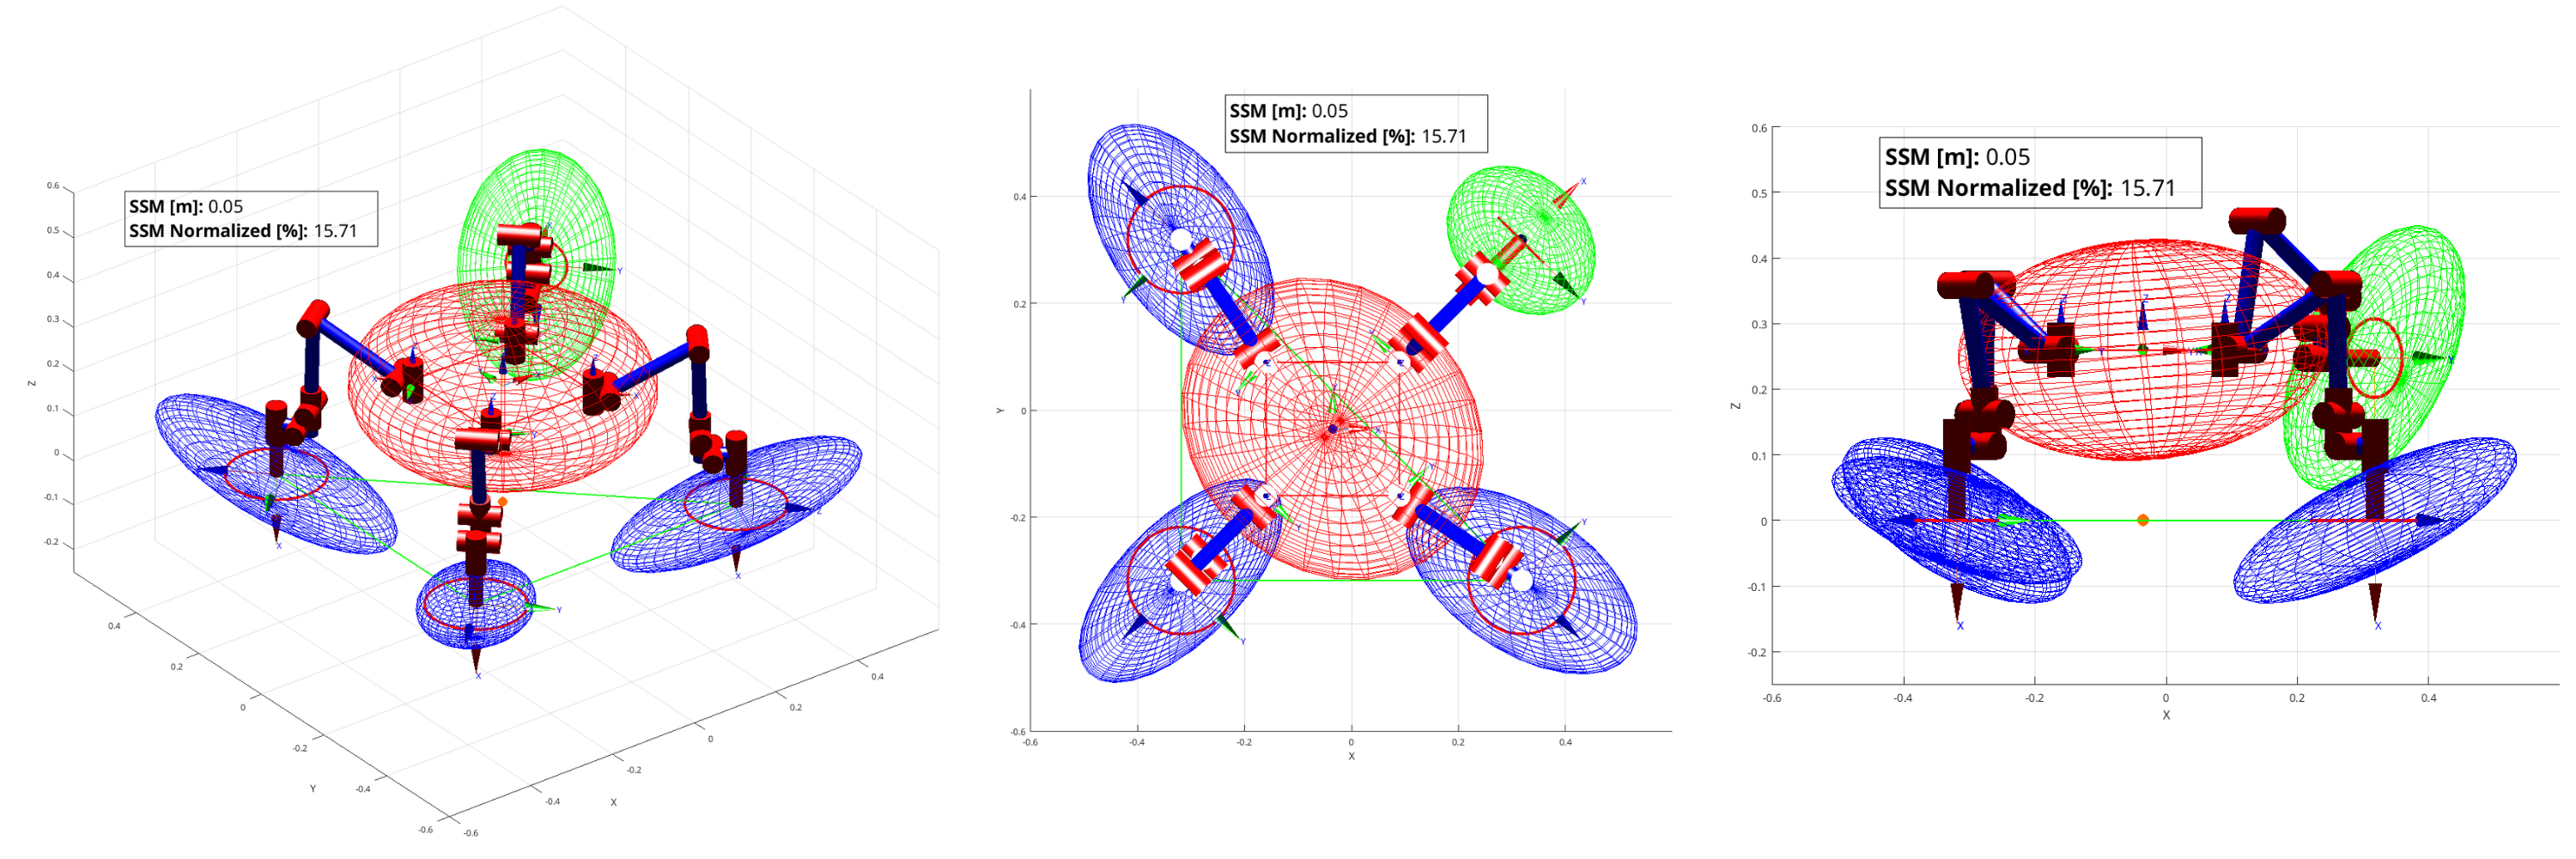
\includegraphics[width=0.9\textwidth]{Images/img_ch5/step3_ruleofthumb.png}} 
    \\
    \subfloat[Limb down\label{fig:down_LF}]{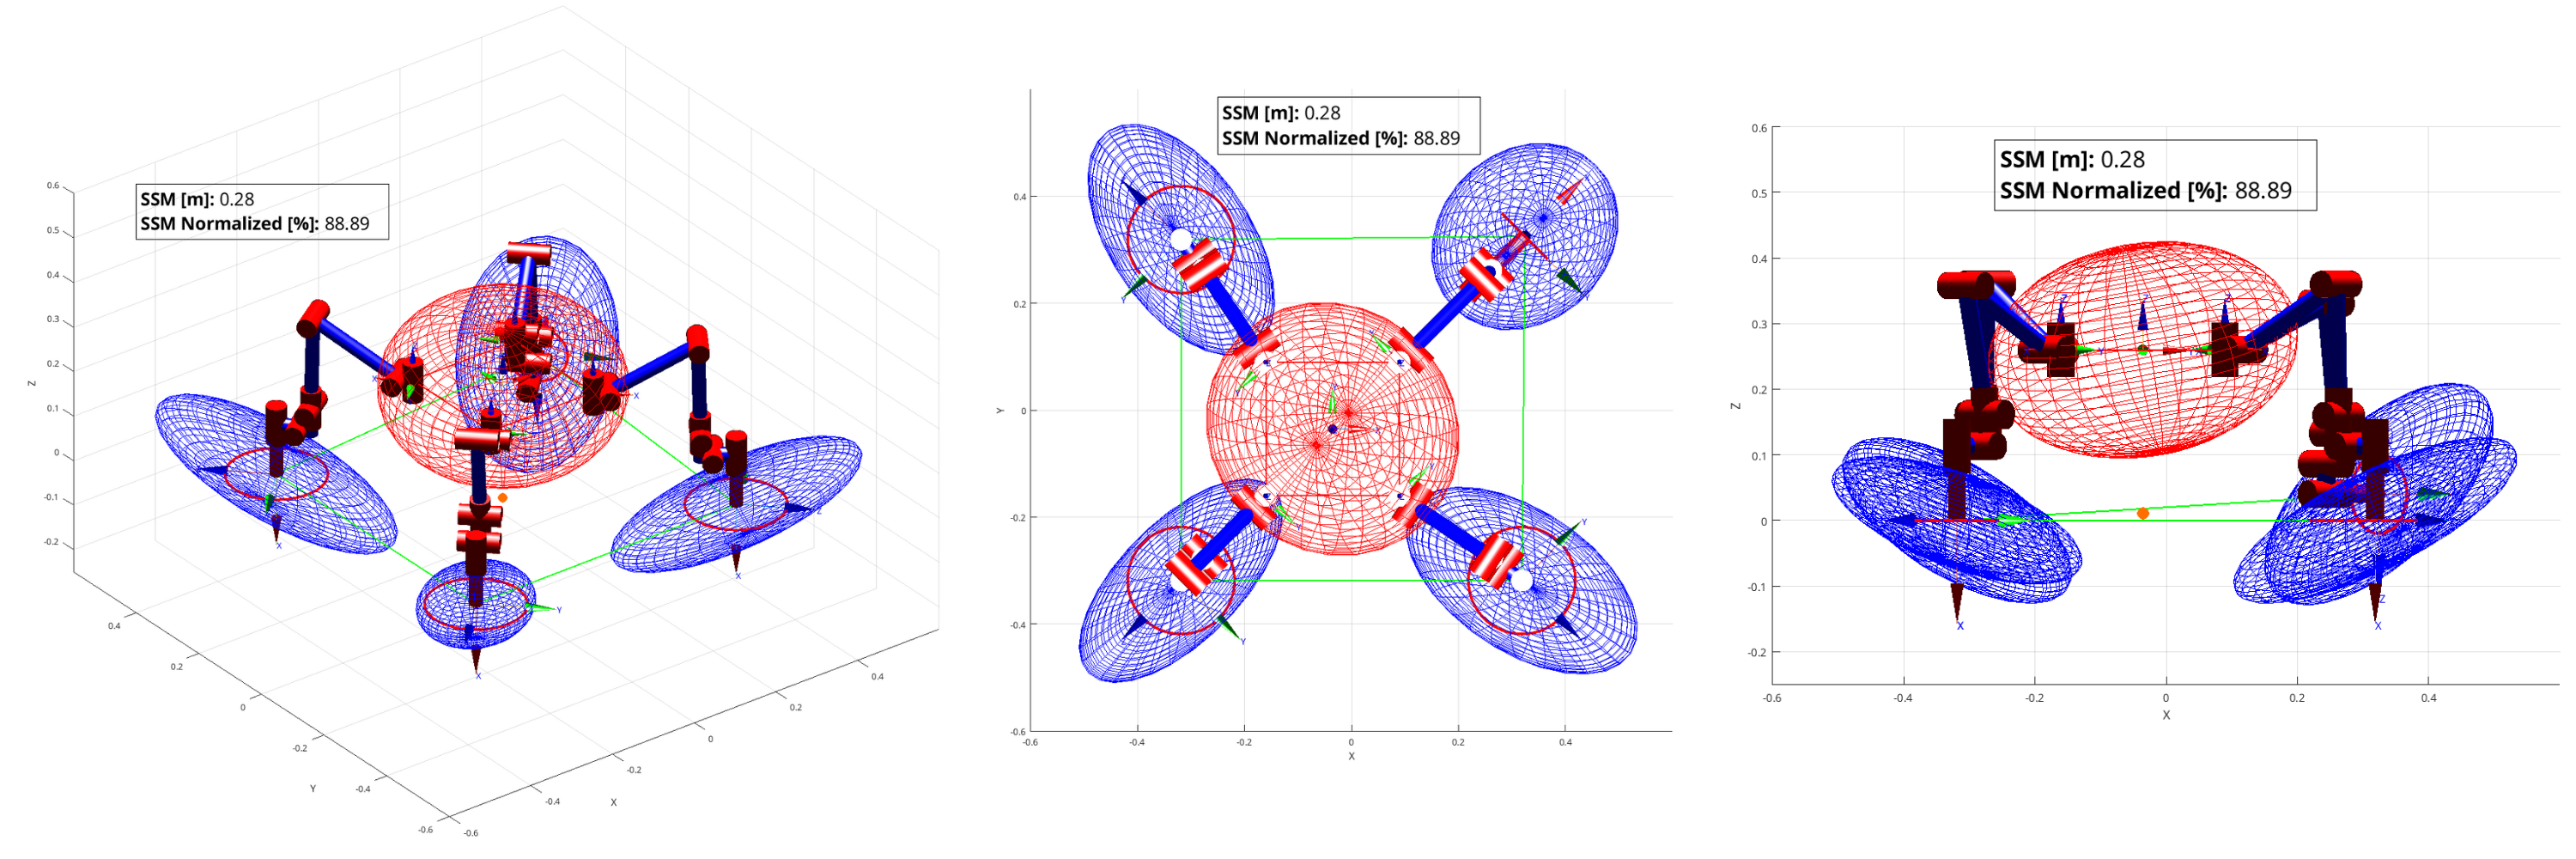
\includegraphics[width=0.9\textwidth]{Images/img_ch5/step4_ruleofthumb.png}} 
    \caption[First limb (LF) transition sequence, rule of thumb]{First limb (LF) transition sequence, with the rule of thumb base motion (perspective, xy, and xz view) }
    \label{fig:G2W_analysis_LF}
\end{figure}

\begin{figure}[H]
    \centering
    \subfloat[Next support polygon estimation\label{fig:support_RF}]{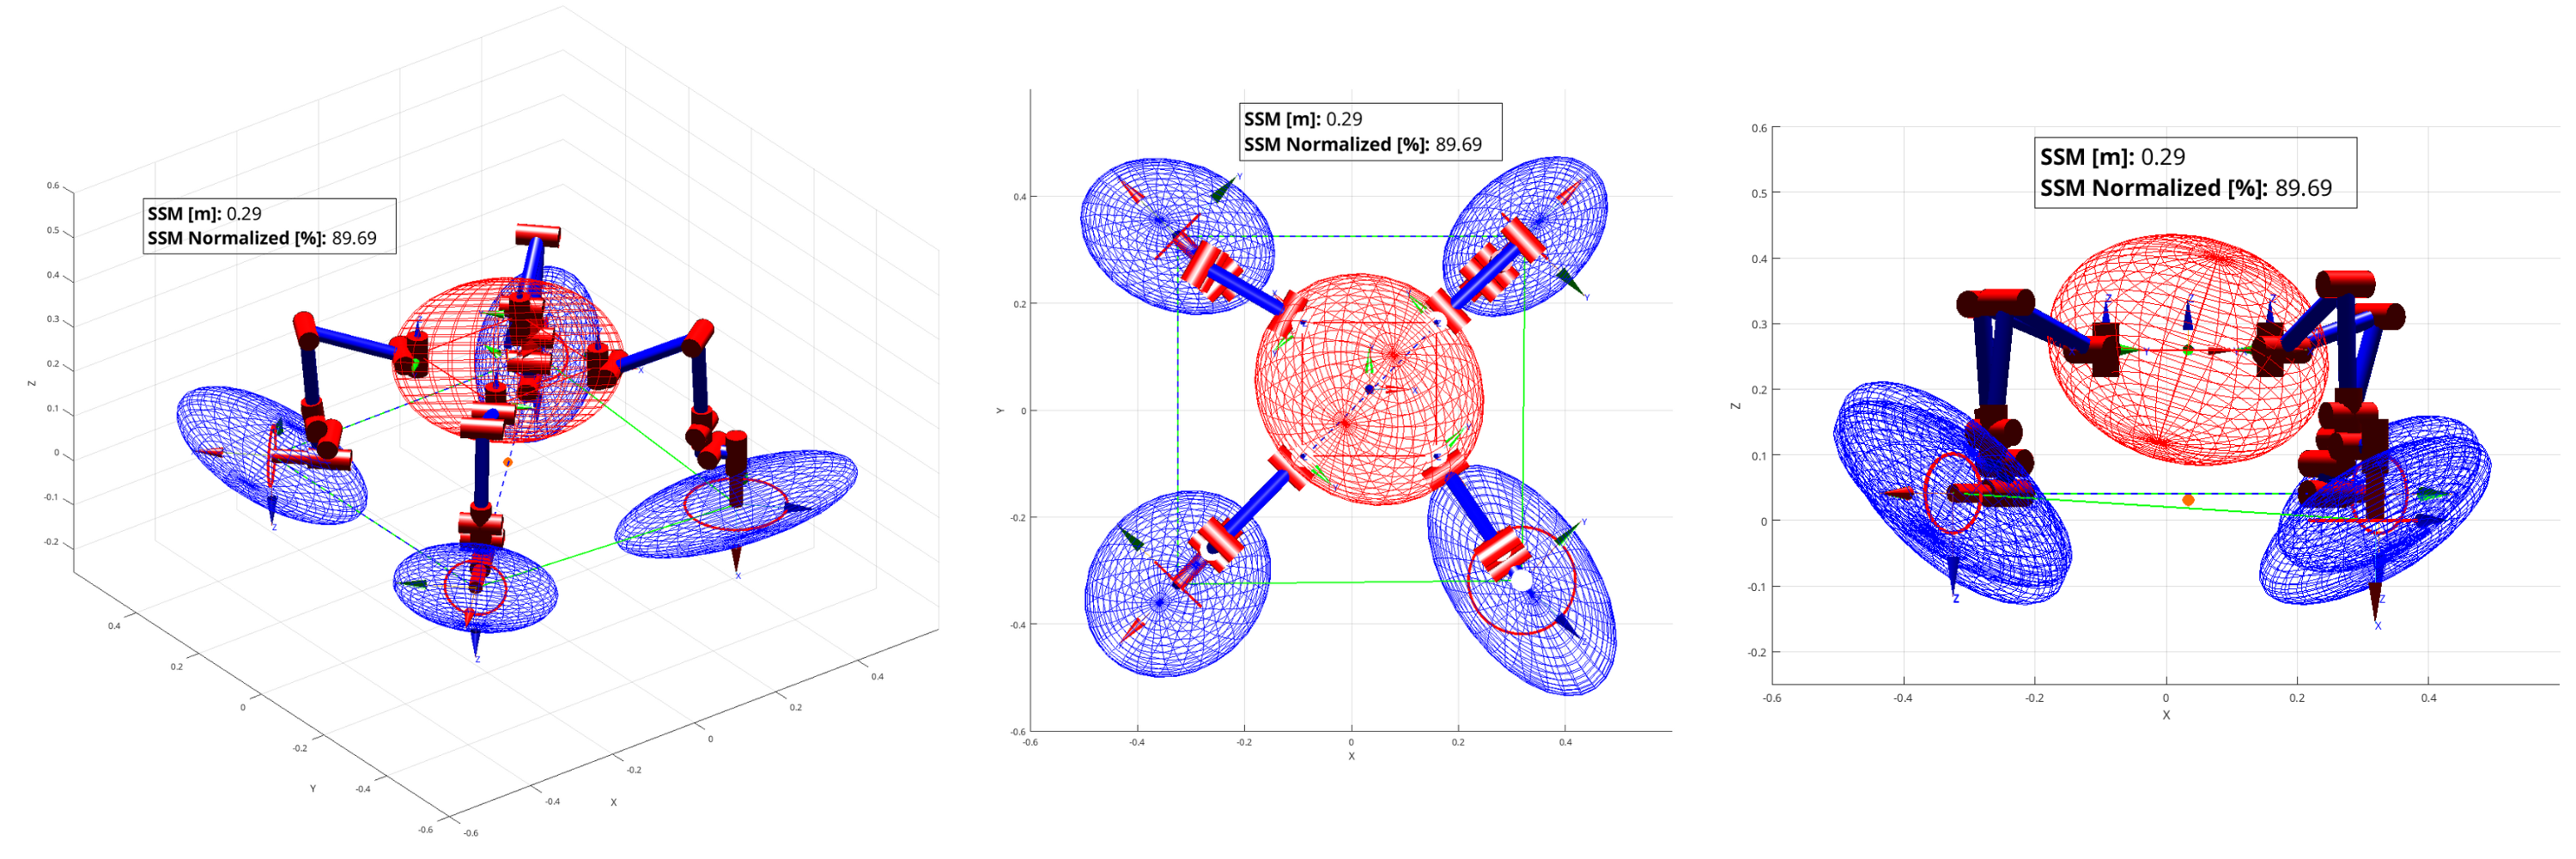
\includegraphics[width=0.9\textwidth]{Images/img_ch5/step5_ruleofthumb.png}} 
    \\
    \subfloat[Base motion task\label{fig:base_RF}]{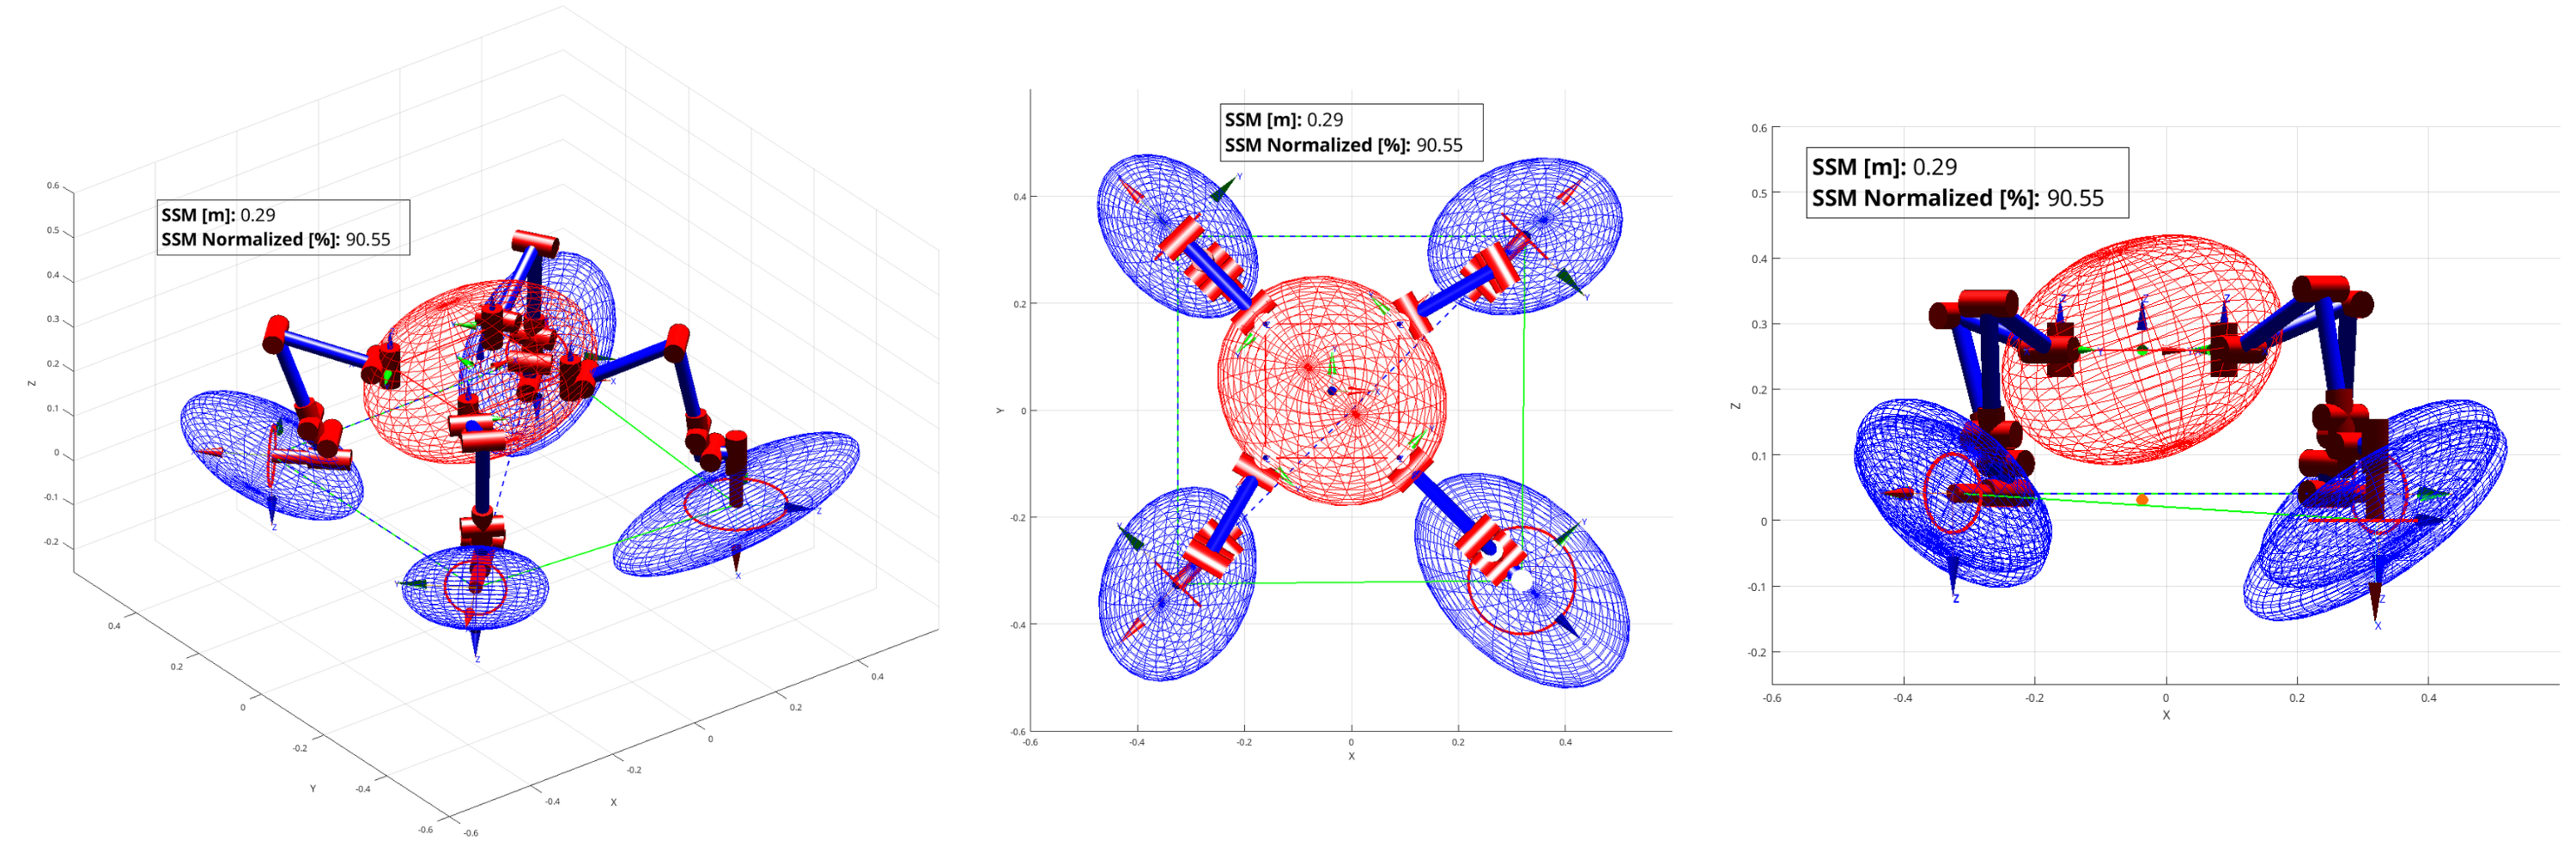
\includegraphics[width=0.9\textwidth]{Images/img_ch5/step6_ruleofthumb.png}} 
    \\
    \subfloat[Raise limb and GRIEEL transformation\label{fig:raise_RF}]{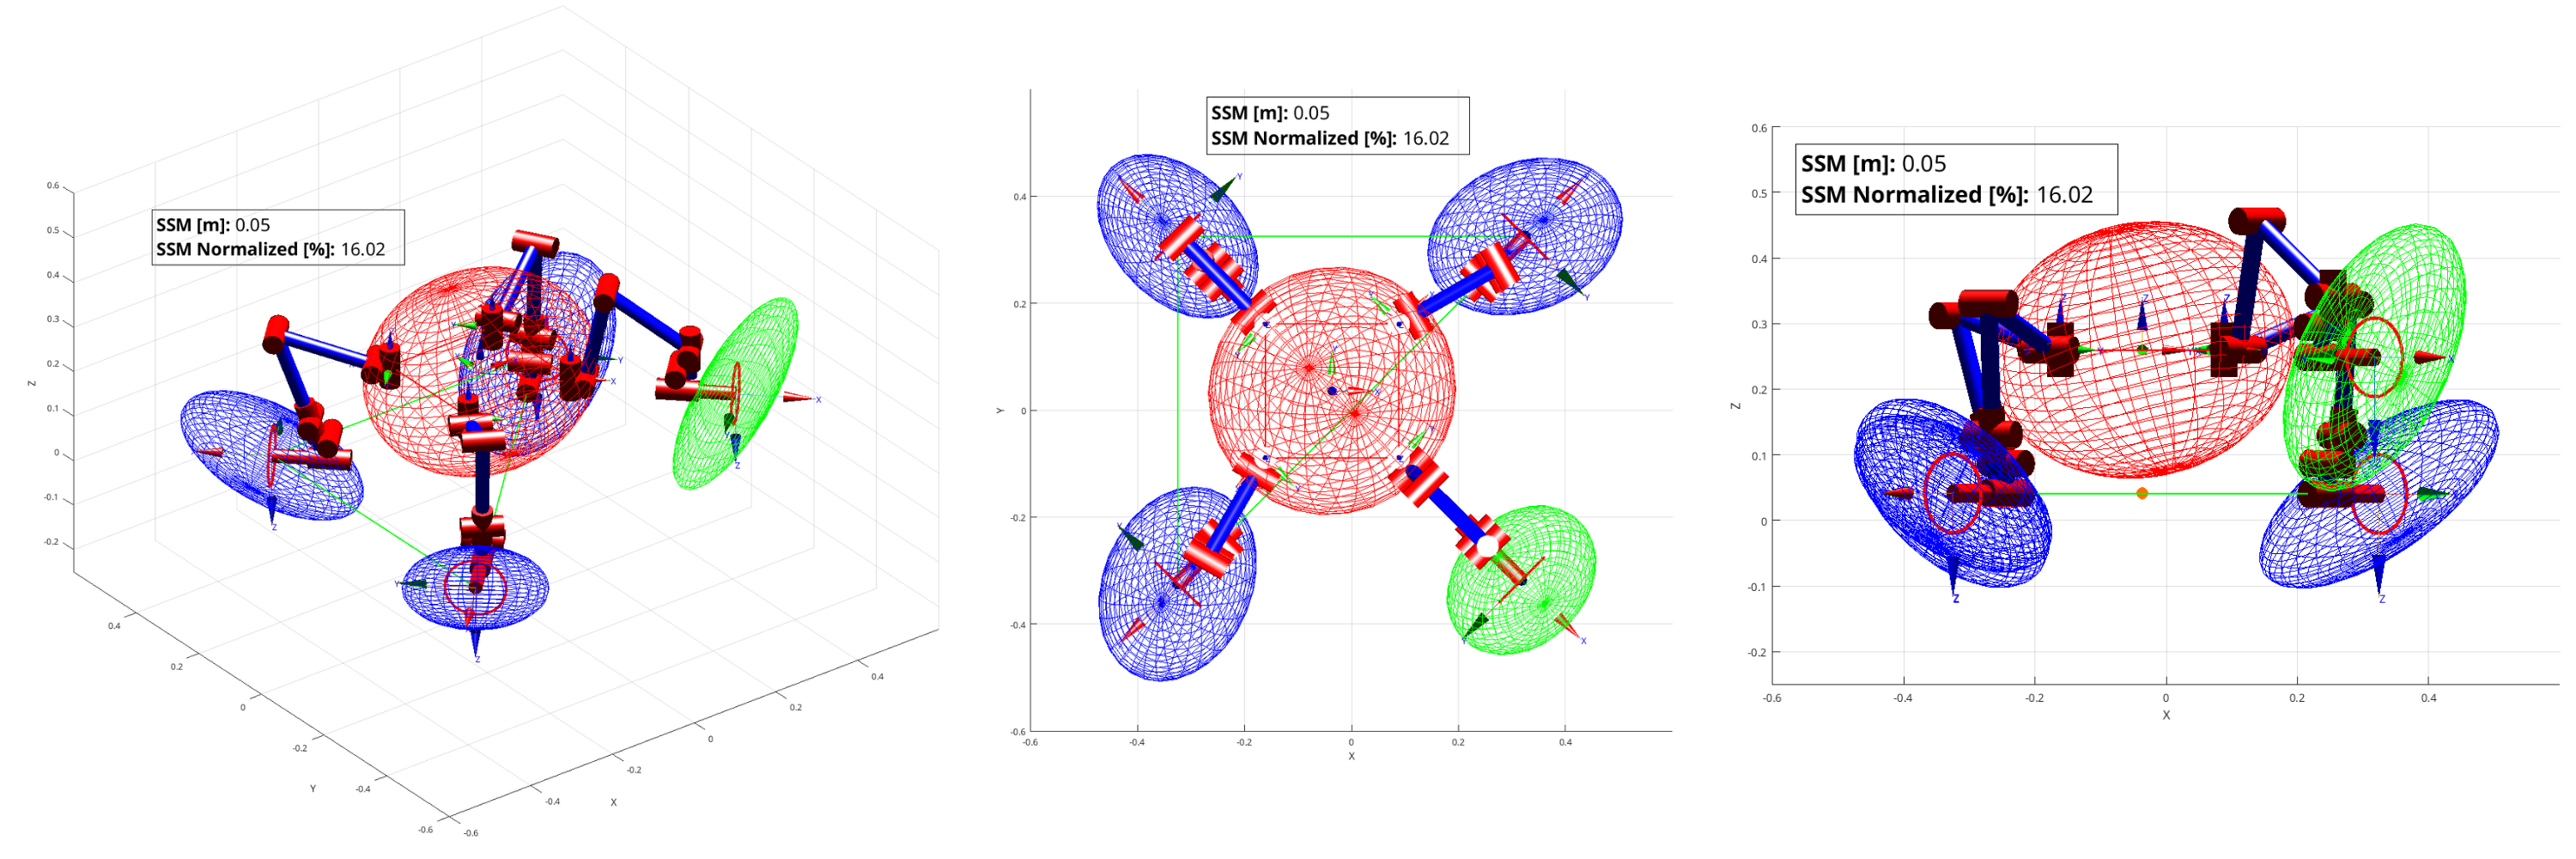
\includegraphics[width=0.9\textwidth]{Images/img_ch5/step7_ruleofthumb.png}} 
    \\
    \subfloat[Limb down\label{fig:down_RF}]{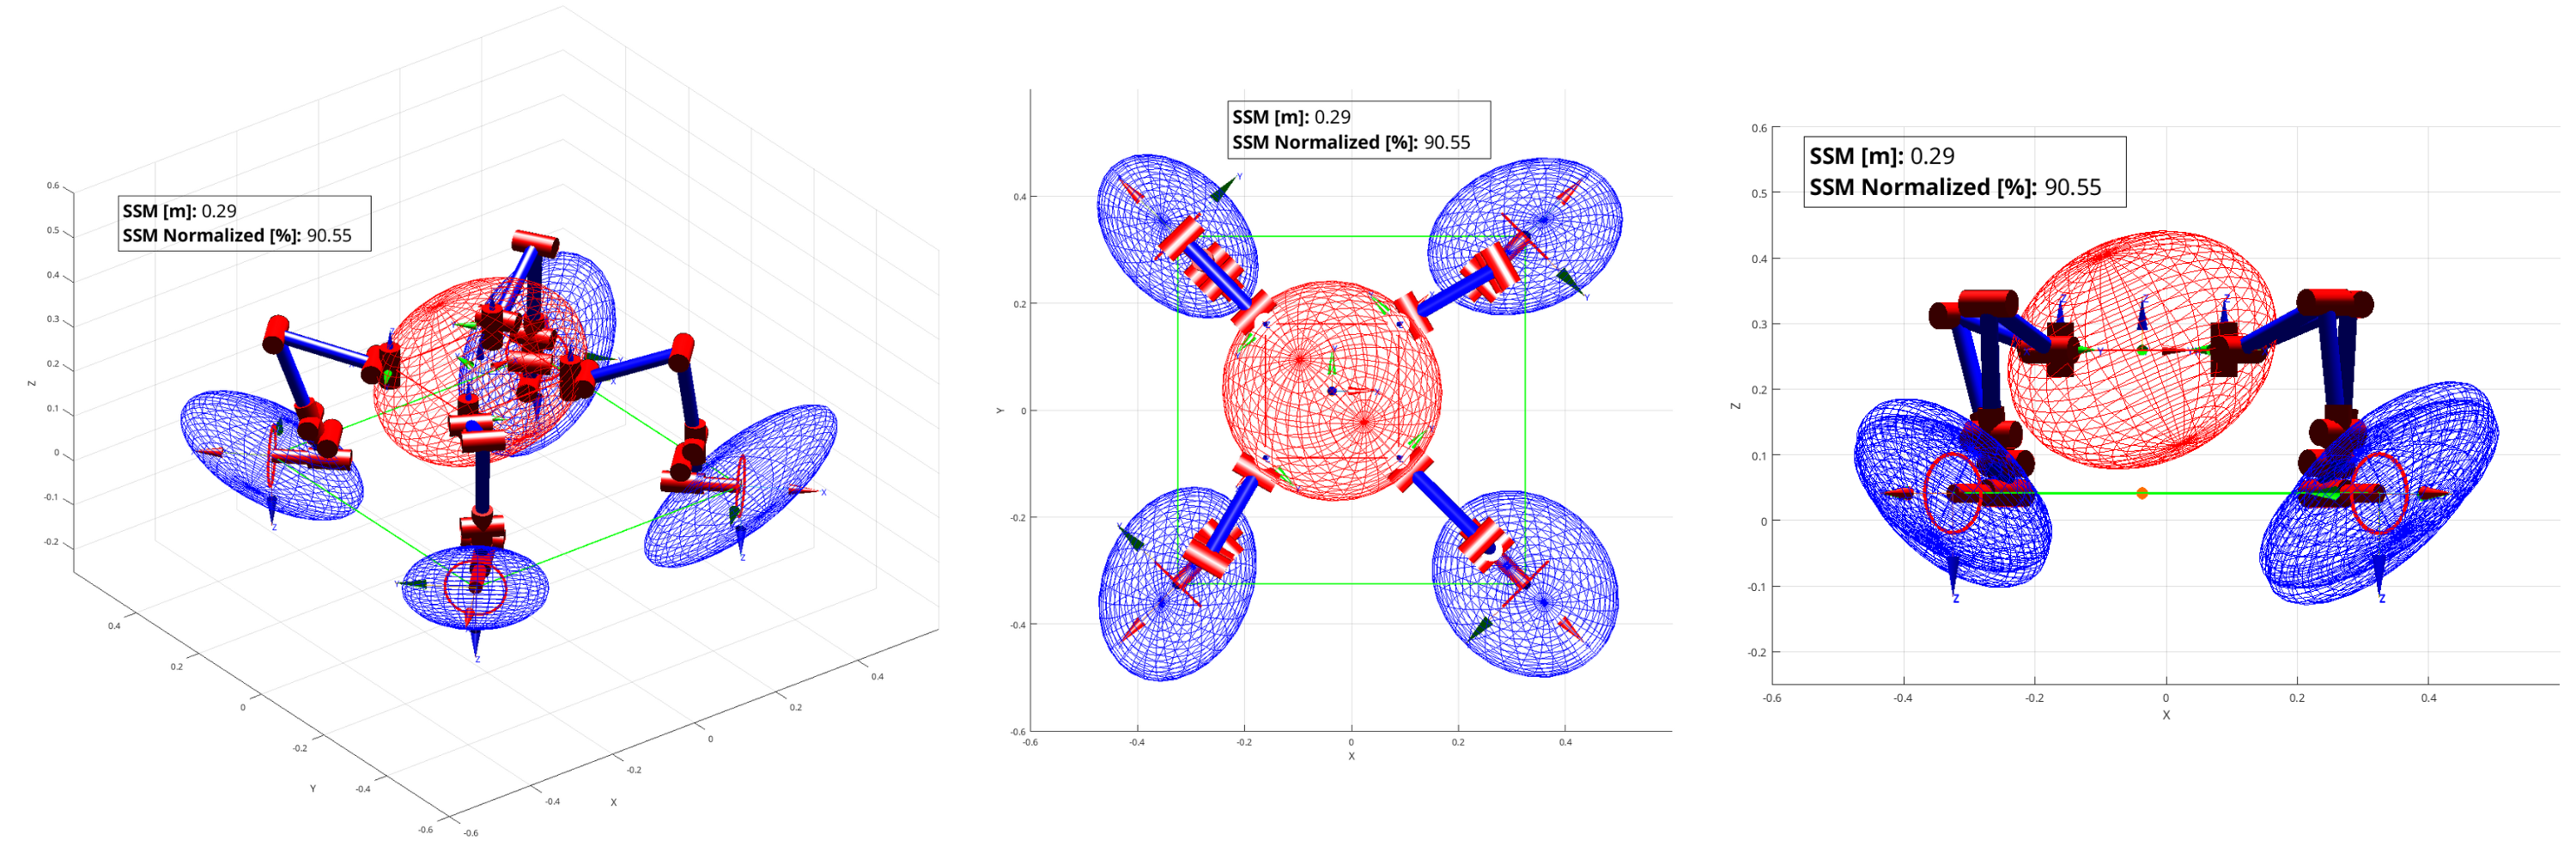
\includegraphics[width=0.9\textwidth]{Images/img_ch5/step8_ruleofthumb.png}} 
    \caption[Final limb (RF) transition sequence, rule of thumb]{Final limb (RF) transition sequence, with the rule of thumb base motion (perspective, xy, and xz view)}
    \label{fig:G2W_analysis_RF}
\end{figure}


\begin{figure}[H]
    \centering
    \subfloat[Base motion task\label{fig:base_LF_opt}]{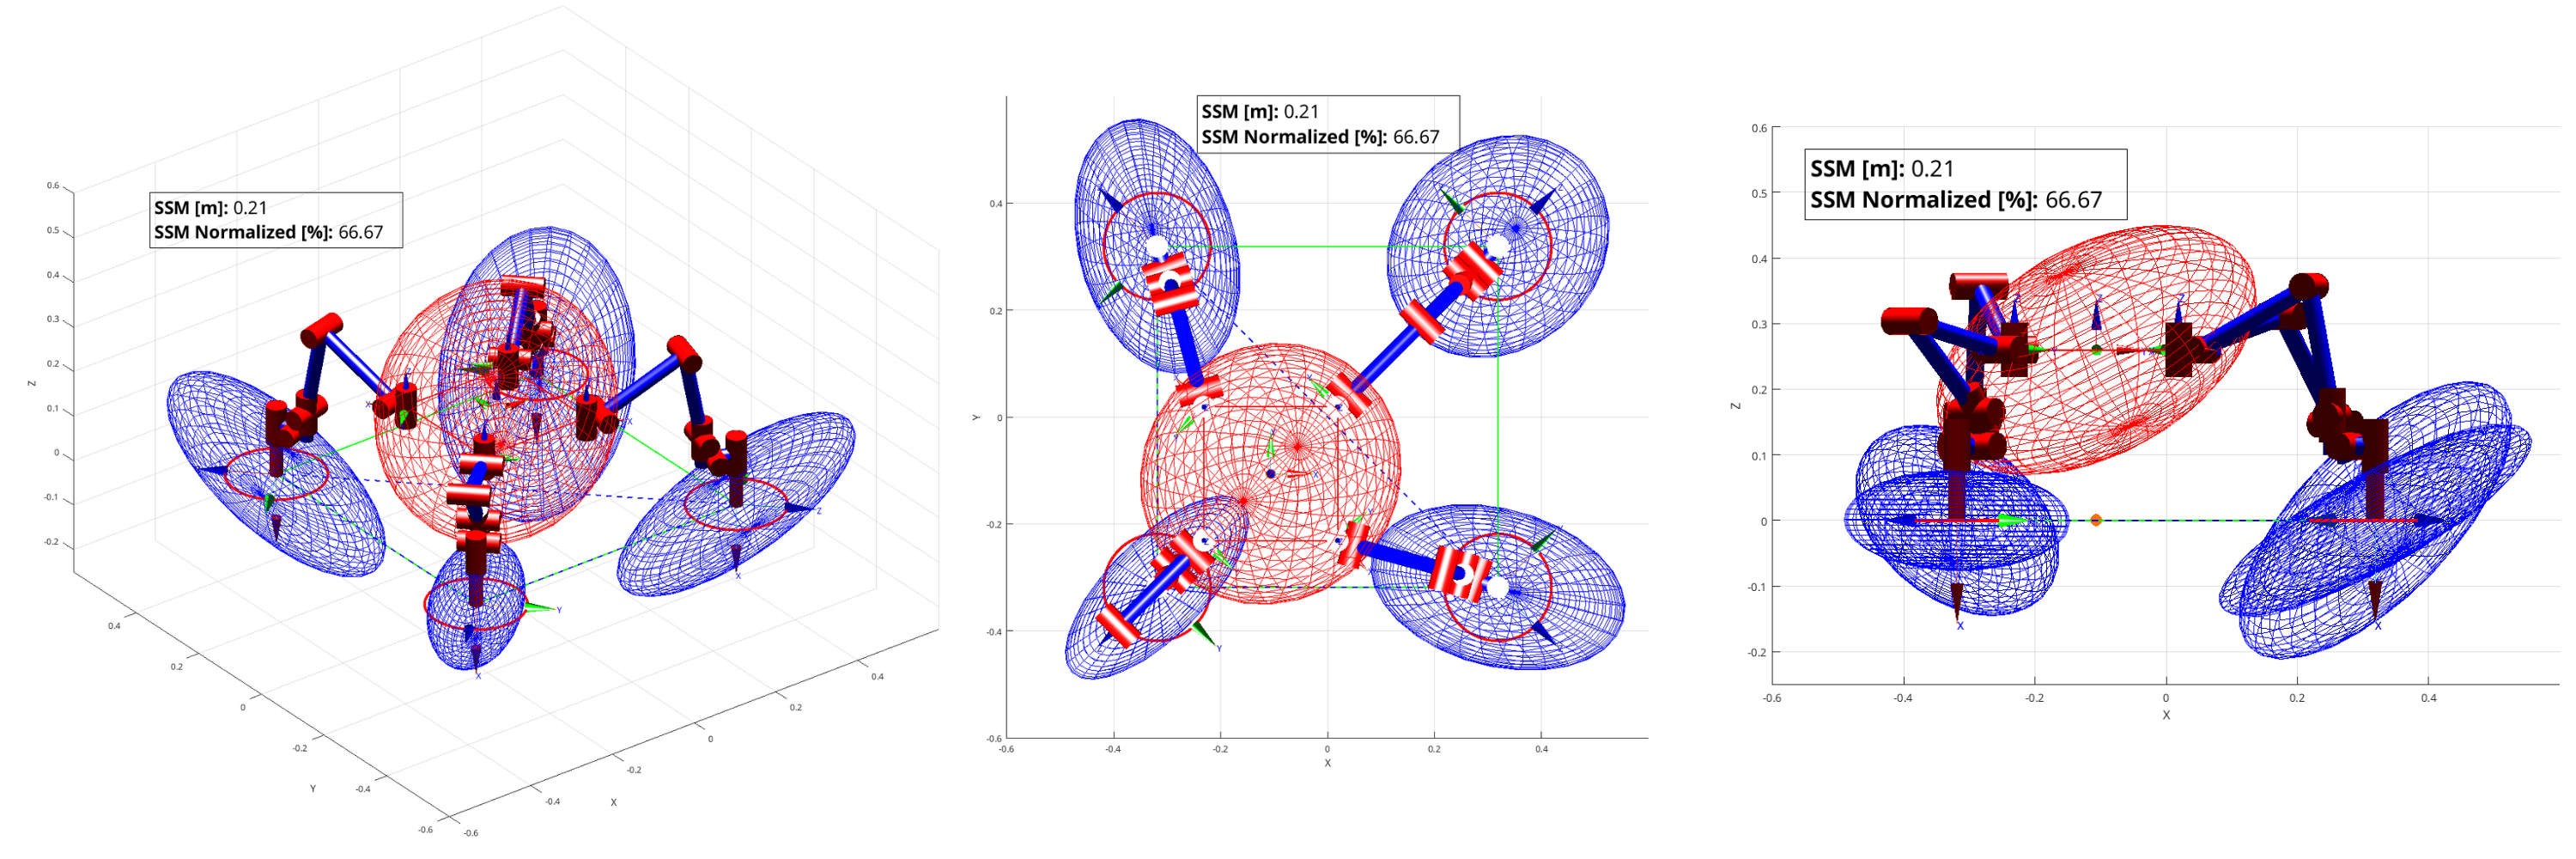
\includegraphics[width=0.9\textwidth]{Images/img_ch5/step2_centering.png}} 
    \\
    \subfloat[Raise limb and GRIEEL transformation\label{fig:raise_LF_opt}]{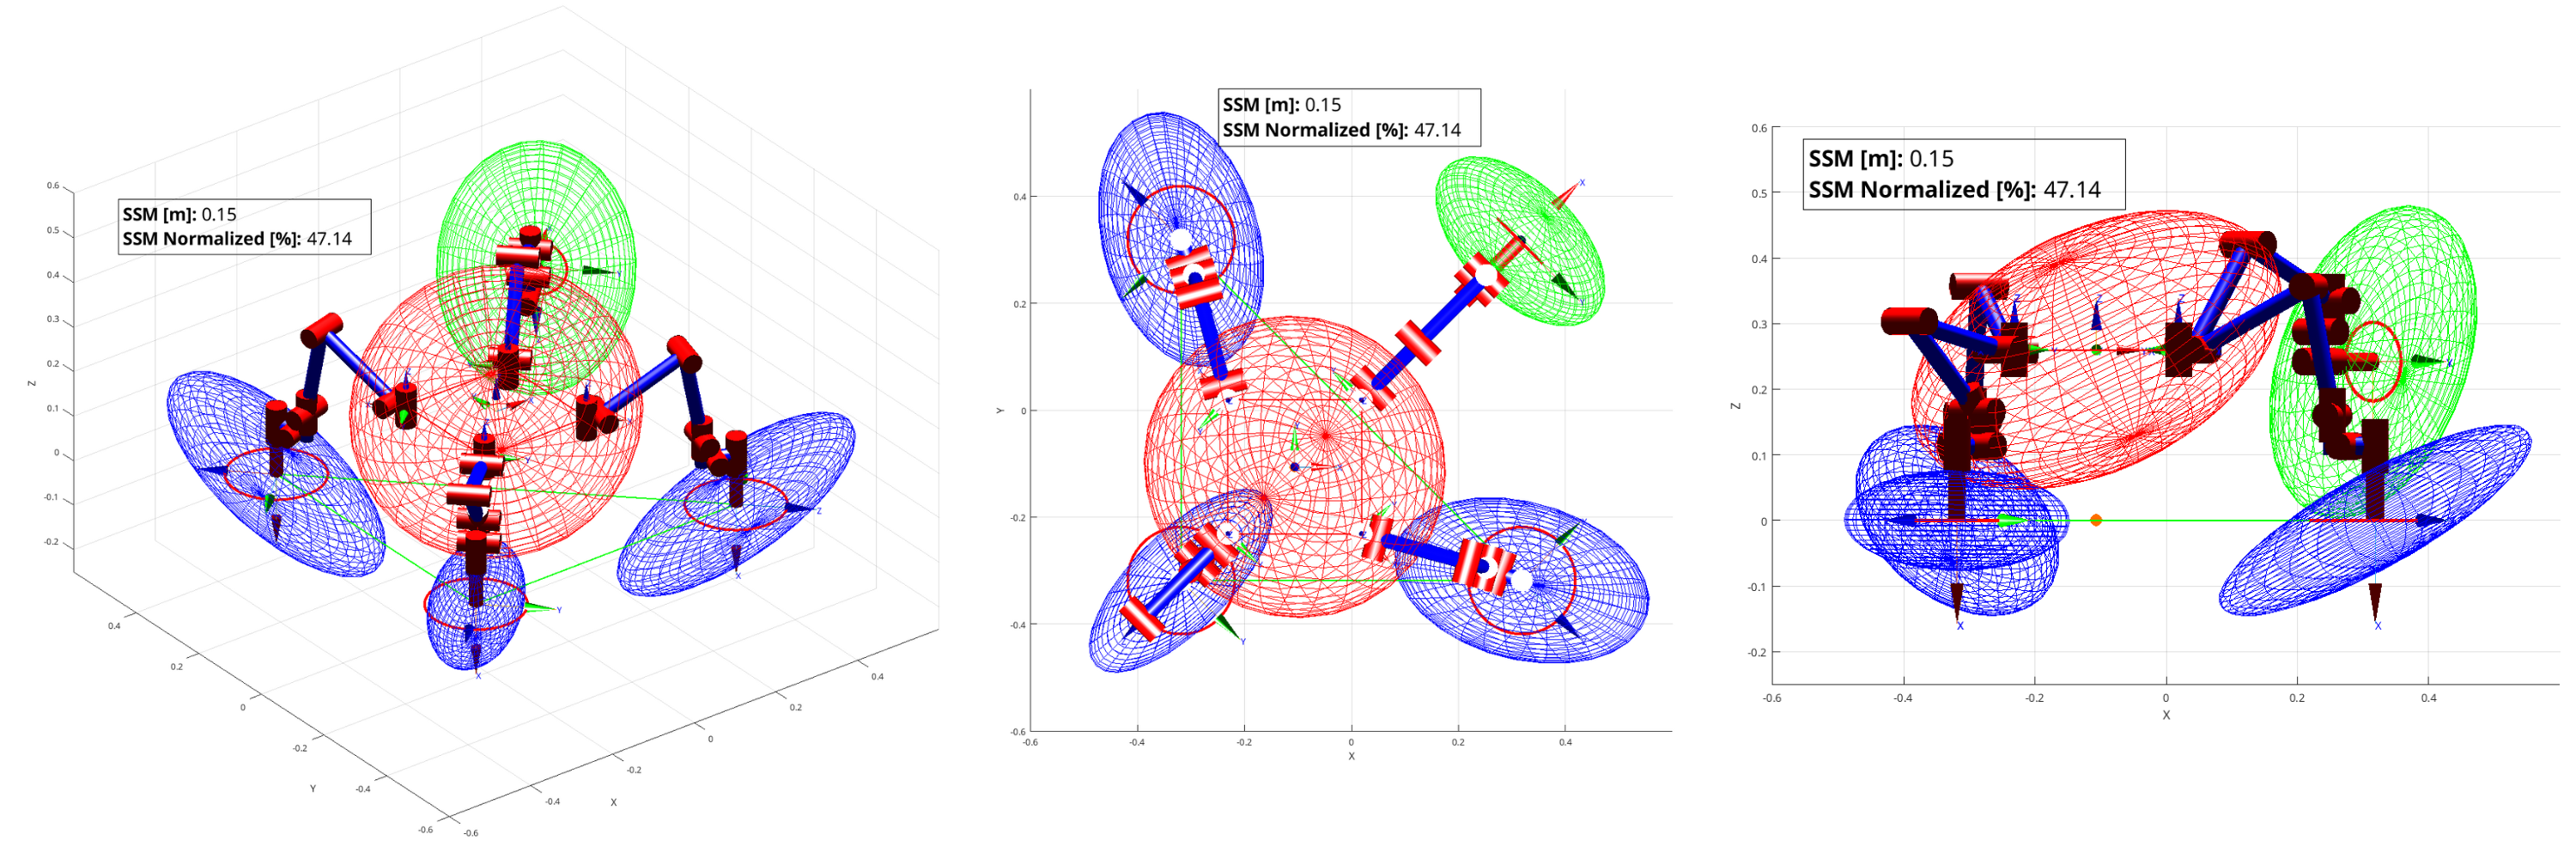
\includegraphics[width=0.9\textwidth]{Images/img_ch5/step3_centering.png}} 
    \\
    \subfloat[Limb down\label{fig:down_LF_opt}]{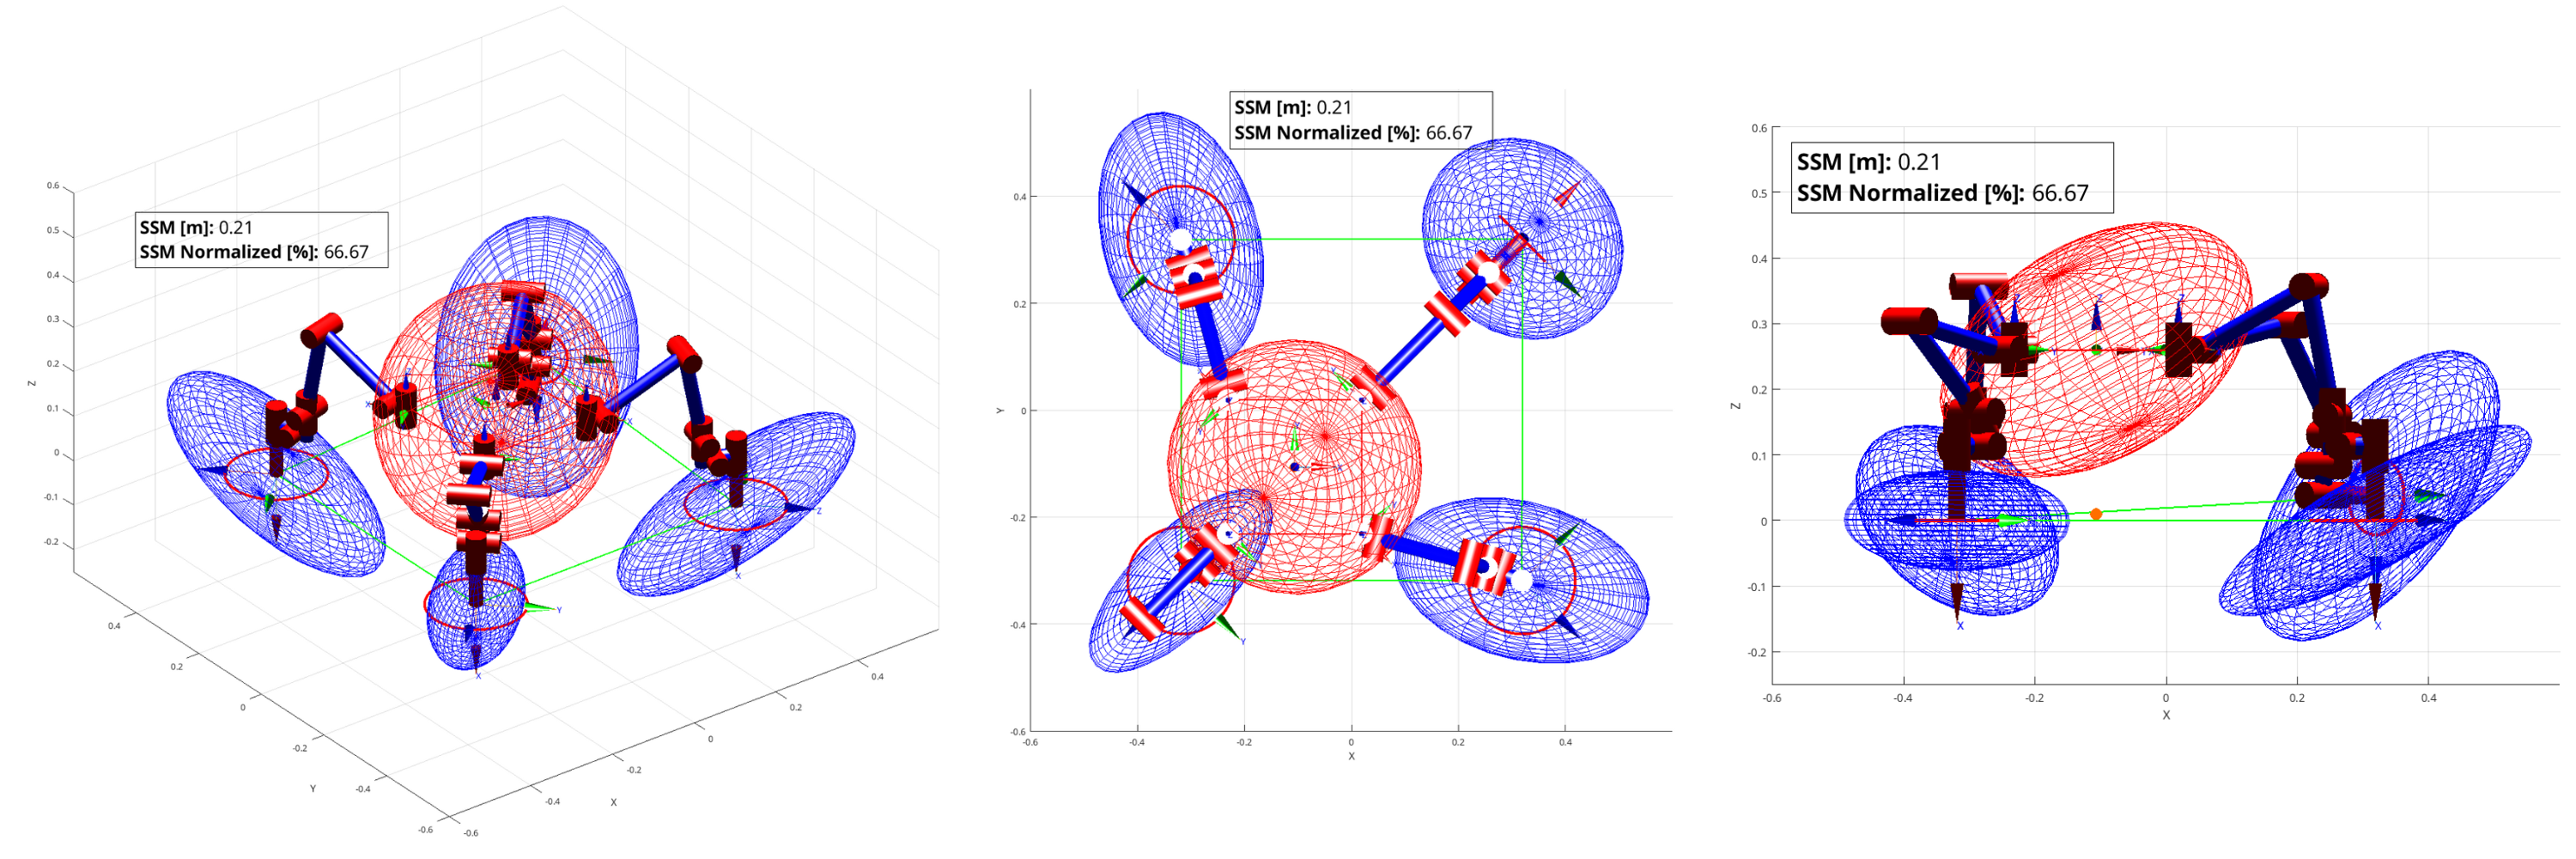
\includegraphics[width=0.9\textwidth]{Images/img_ch5/step4_centering.png}} 
    \caption[First limb (LF) transition sequence, base centering]{First limb (LF) transition sequence, with base centering (perspective, xy, and xz view)}
    \label{fig:G2W_optimal_analysis_LF}
\end{figure}

\begin{figure}[H]
    \centering
    \subfloat[Next support polygon estimation\label{fig:support_RF_opt}]{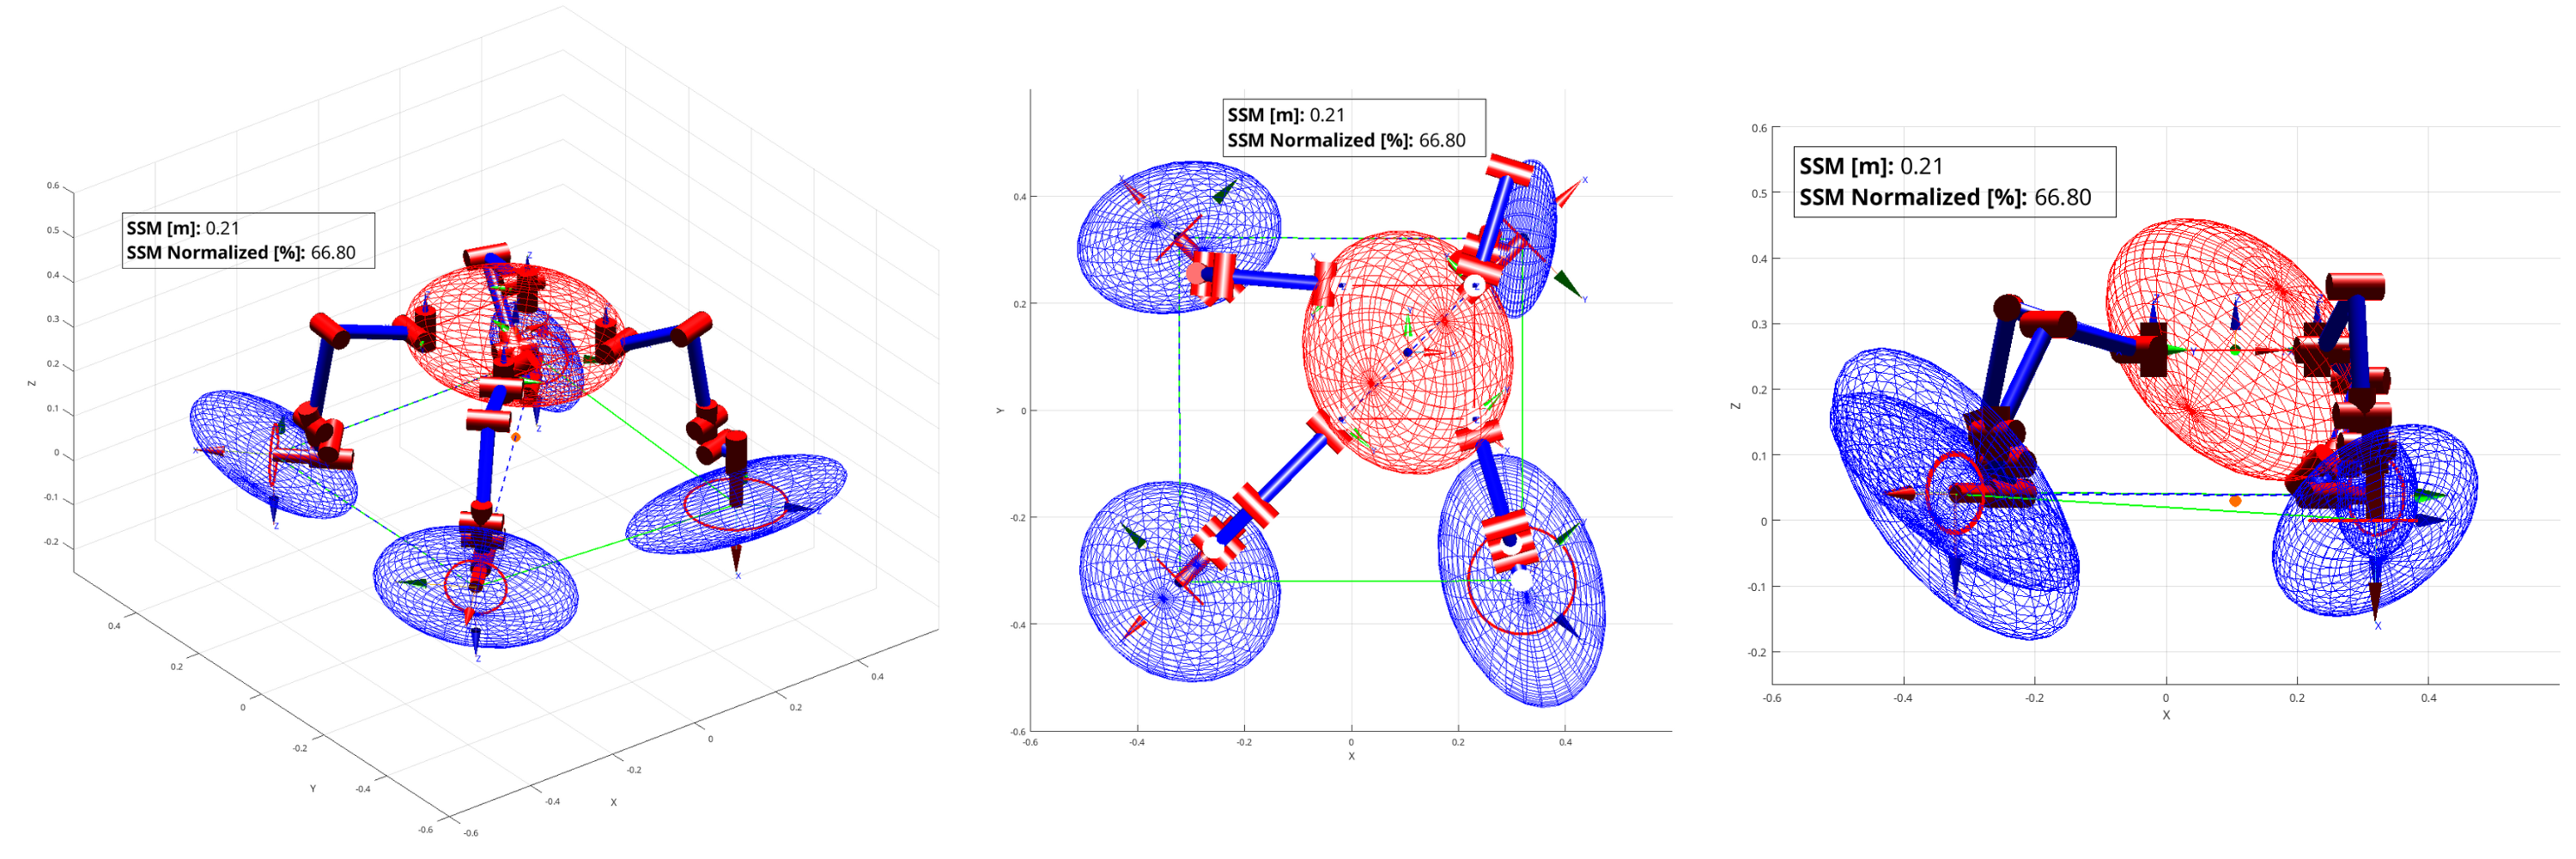
\includegraphics[width=0.9\textwidth]{Images/img_ch5/step5_centering.png}} 
    \\
    \subfloat[Base motion task\label{fig:base_RF_opt}]{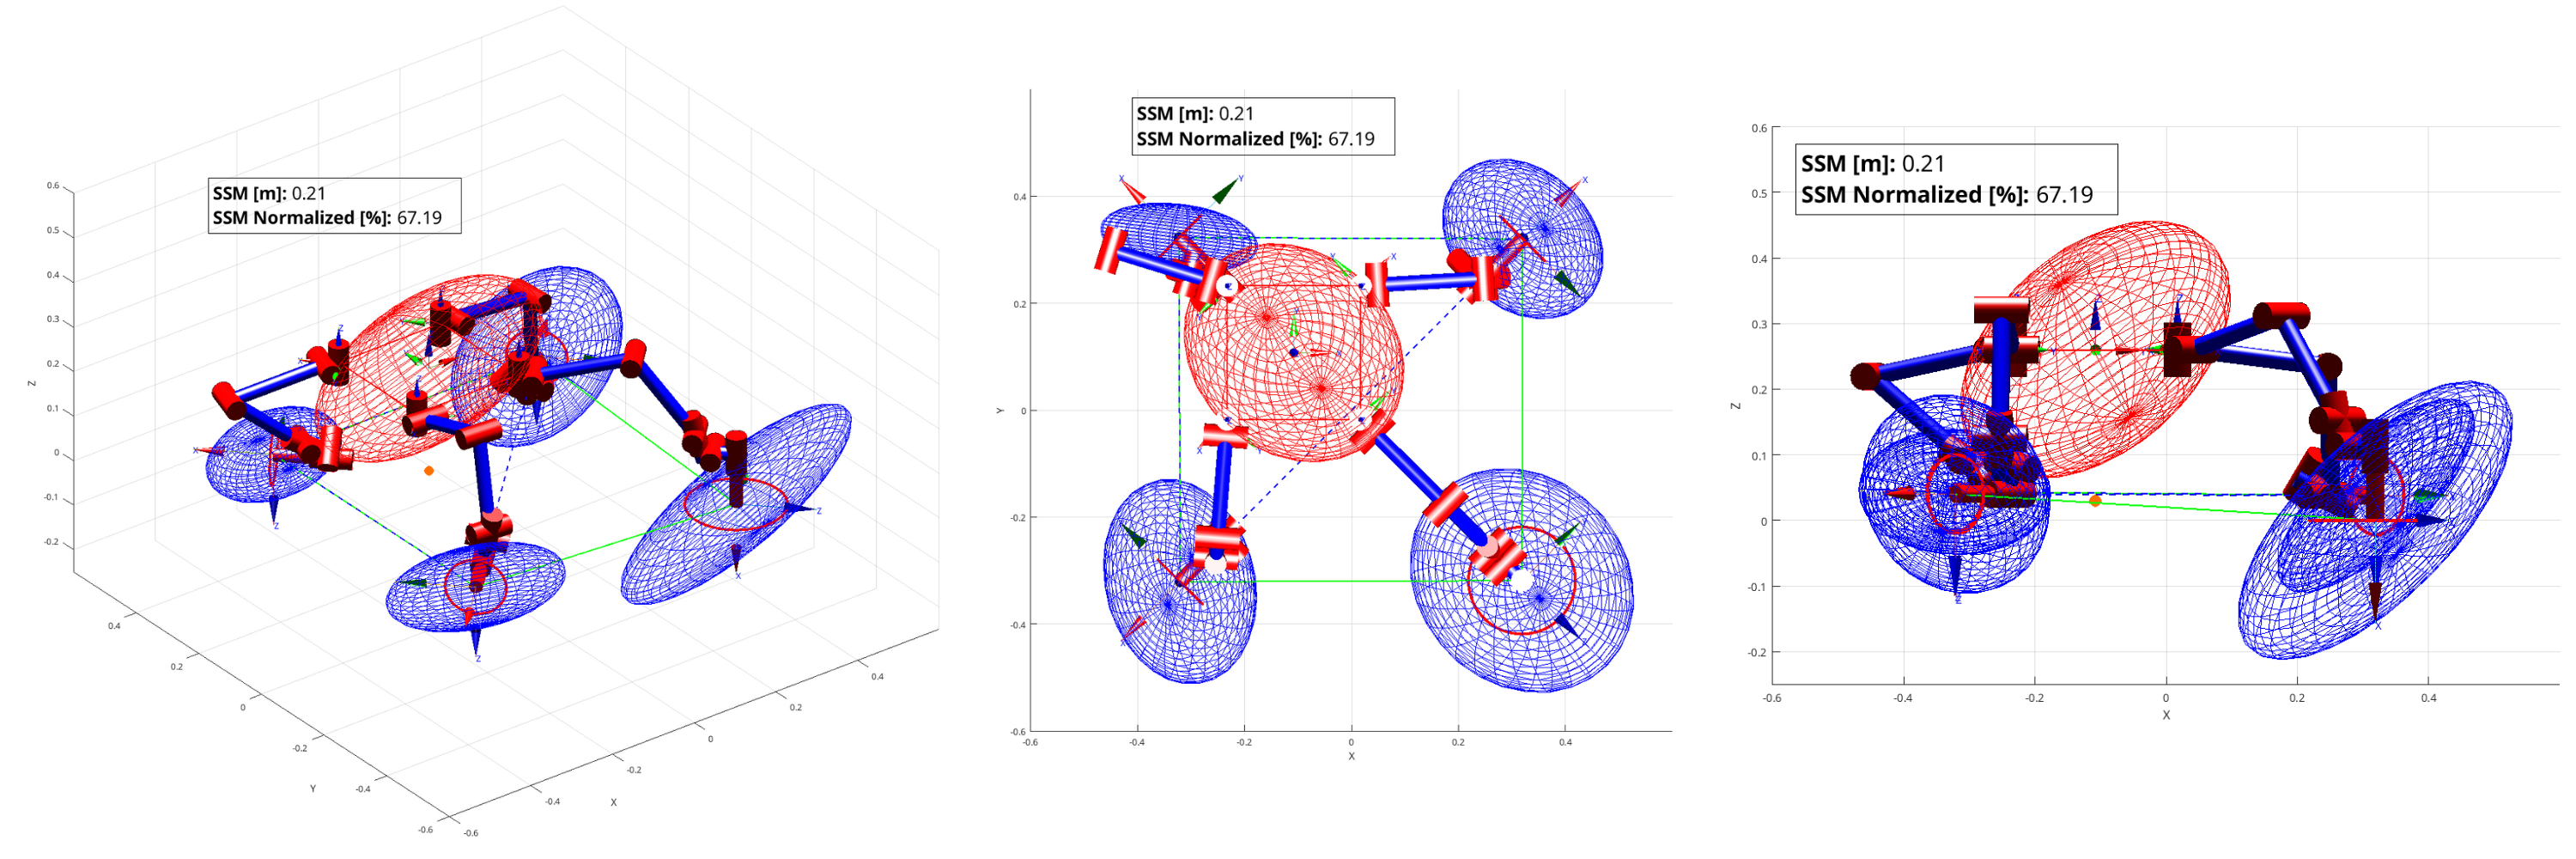
\includegraphics[width=0.9\textwidth]{Images/img_ch5/step6_centering.png}} 
    \\
    \subfloat[Raise limb and GRIEEL transformation\label{fig:raise_RF_opt}]{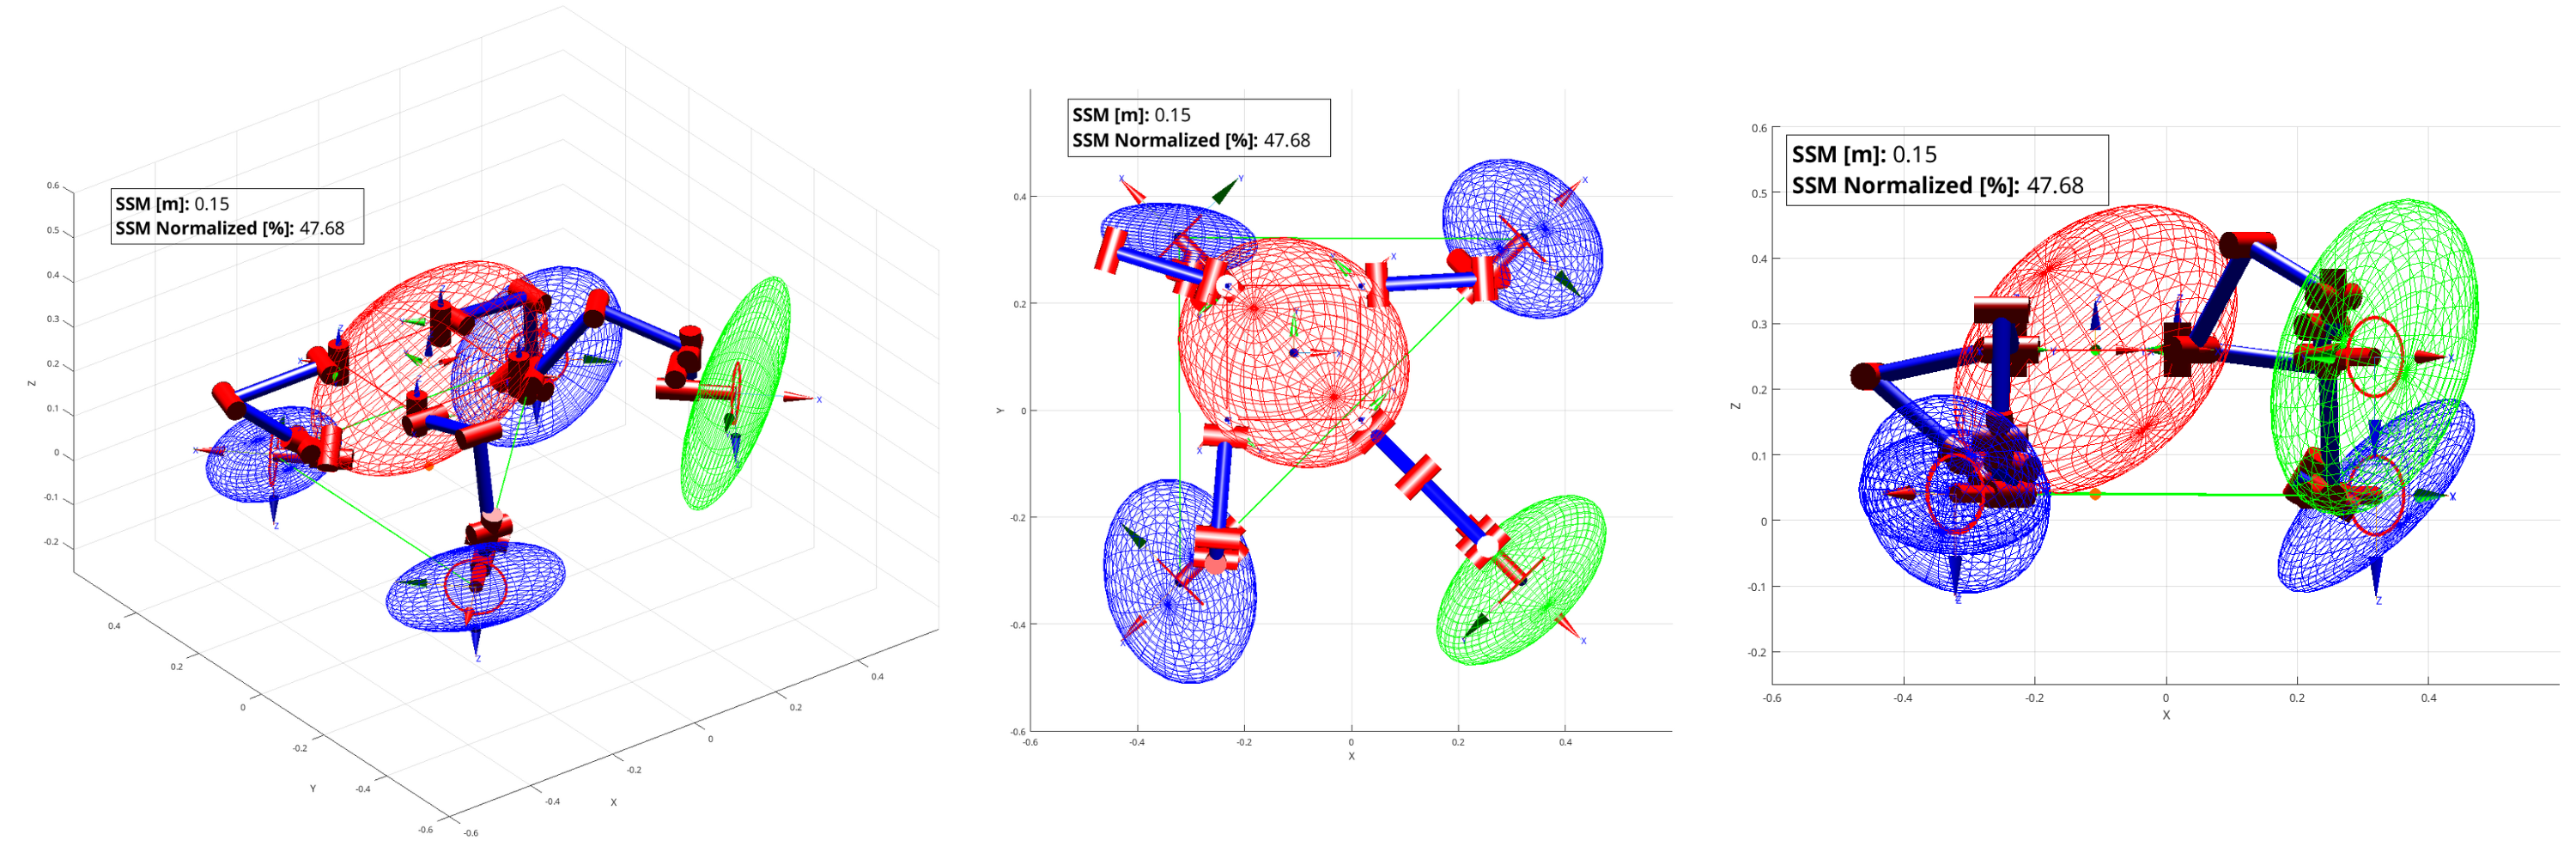
\includegraphics[width=0.9\textwidth]{Images/img_ch5/step7_centering.png}} 
    \\
    \subfloat[Limb down\label{fig:down_RF_opt}]{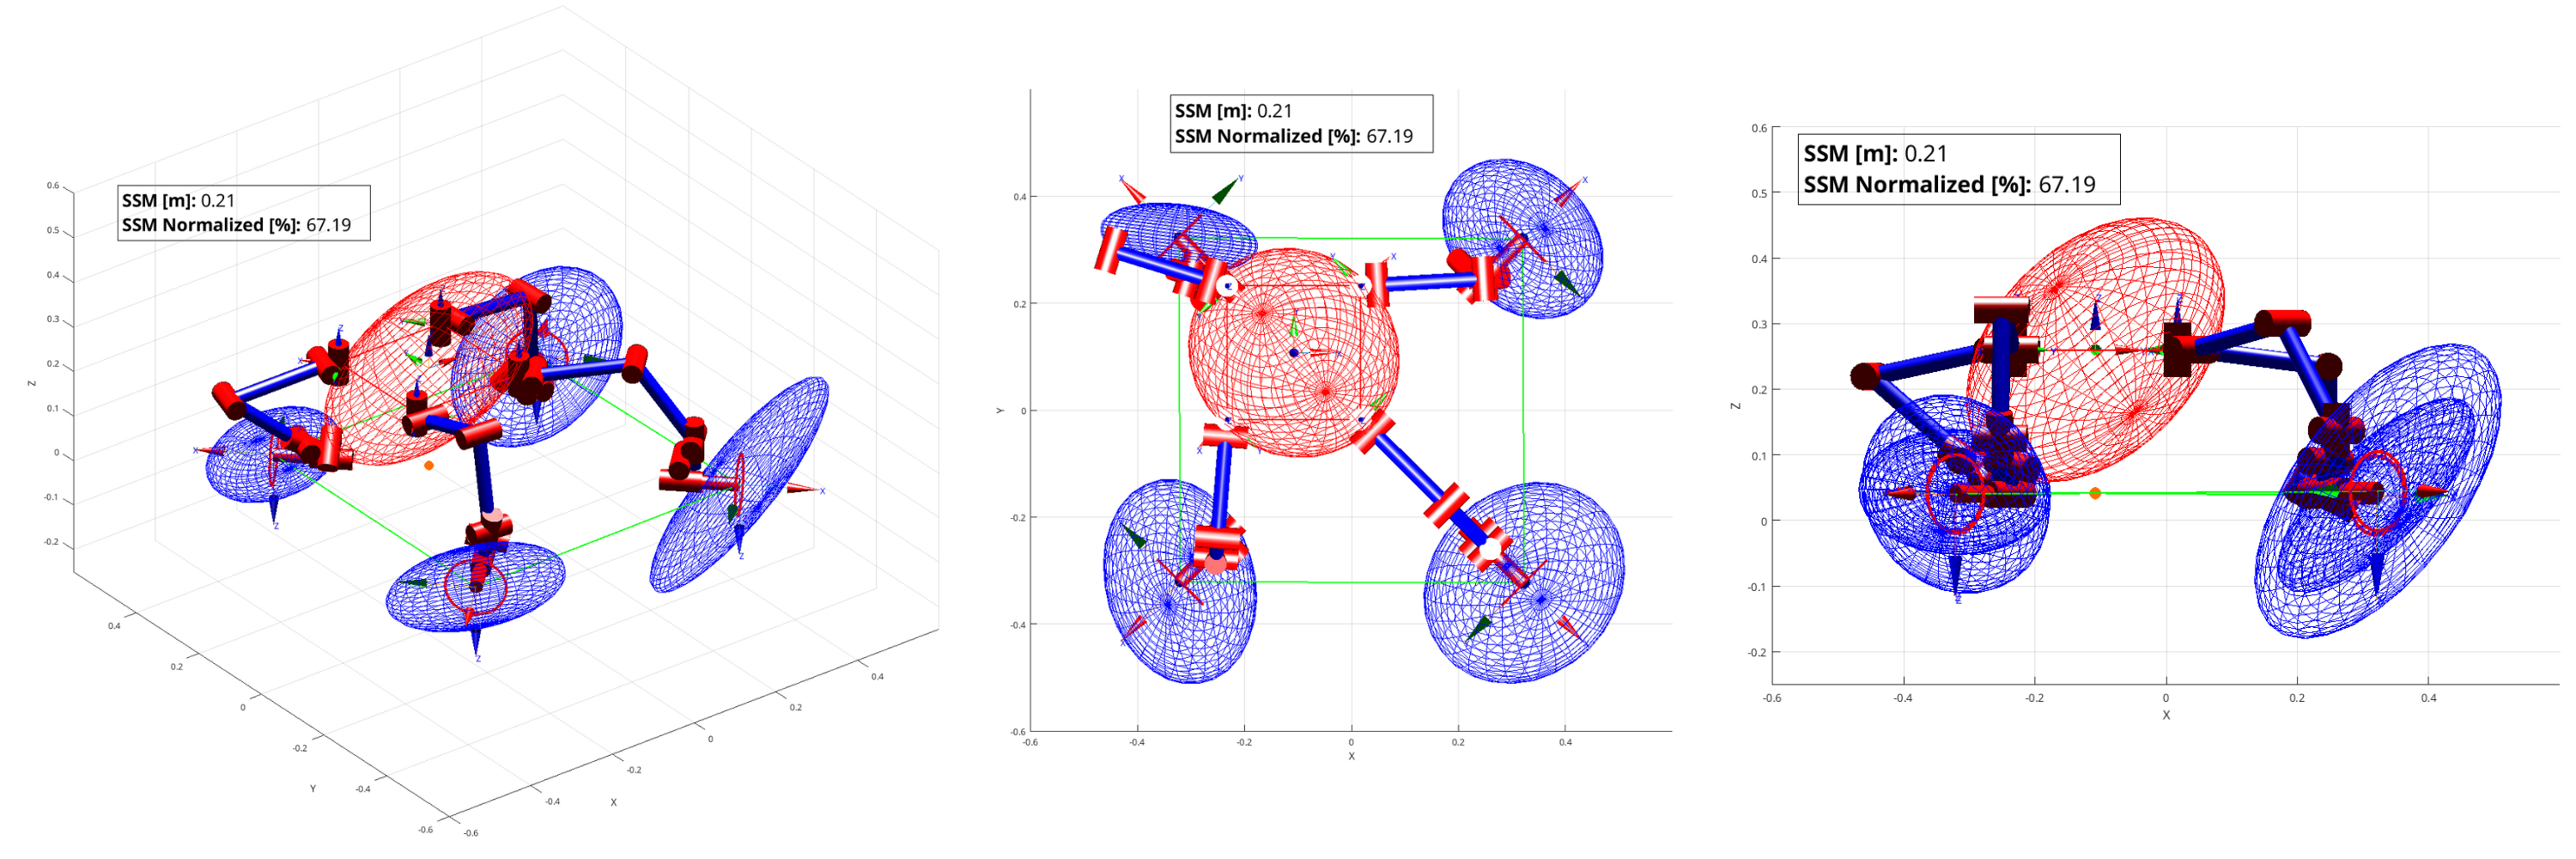
\includegraphics[width=0.9\textwidth]{Images/img_ch5/step8_centering.png}} 
    \caption[Final limb (RF)transition sequence, base centering]{Final limb (RF) transition sequence, with base centering (perspective, xy, and xz view)}
    \label{fig:G2W_optimal_analysis_RF}
\end{figure}

\begin{figure}[H]
    \centering
    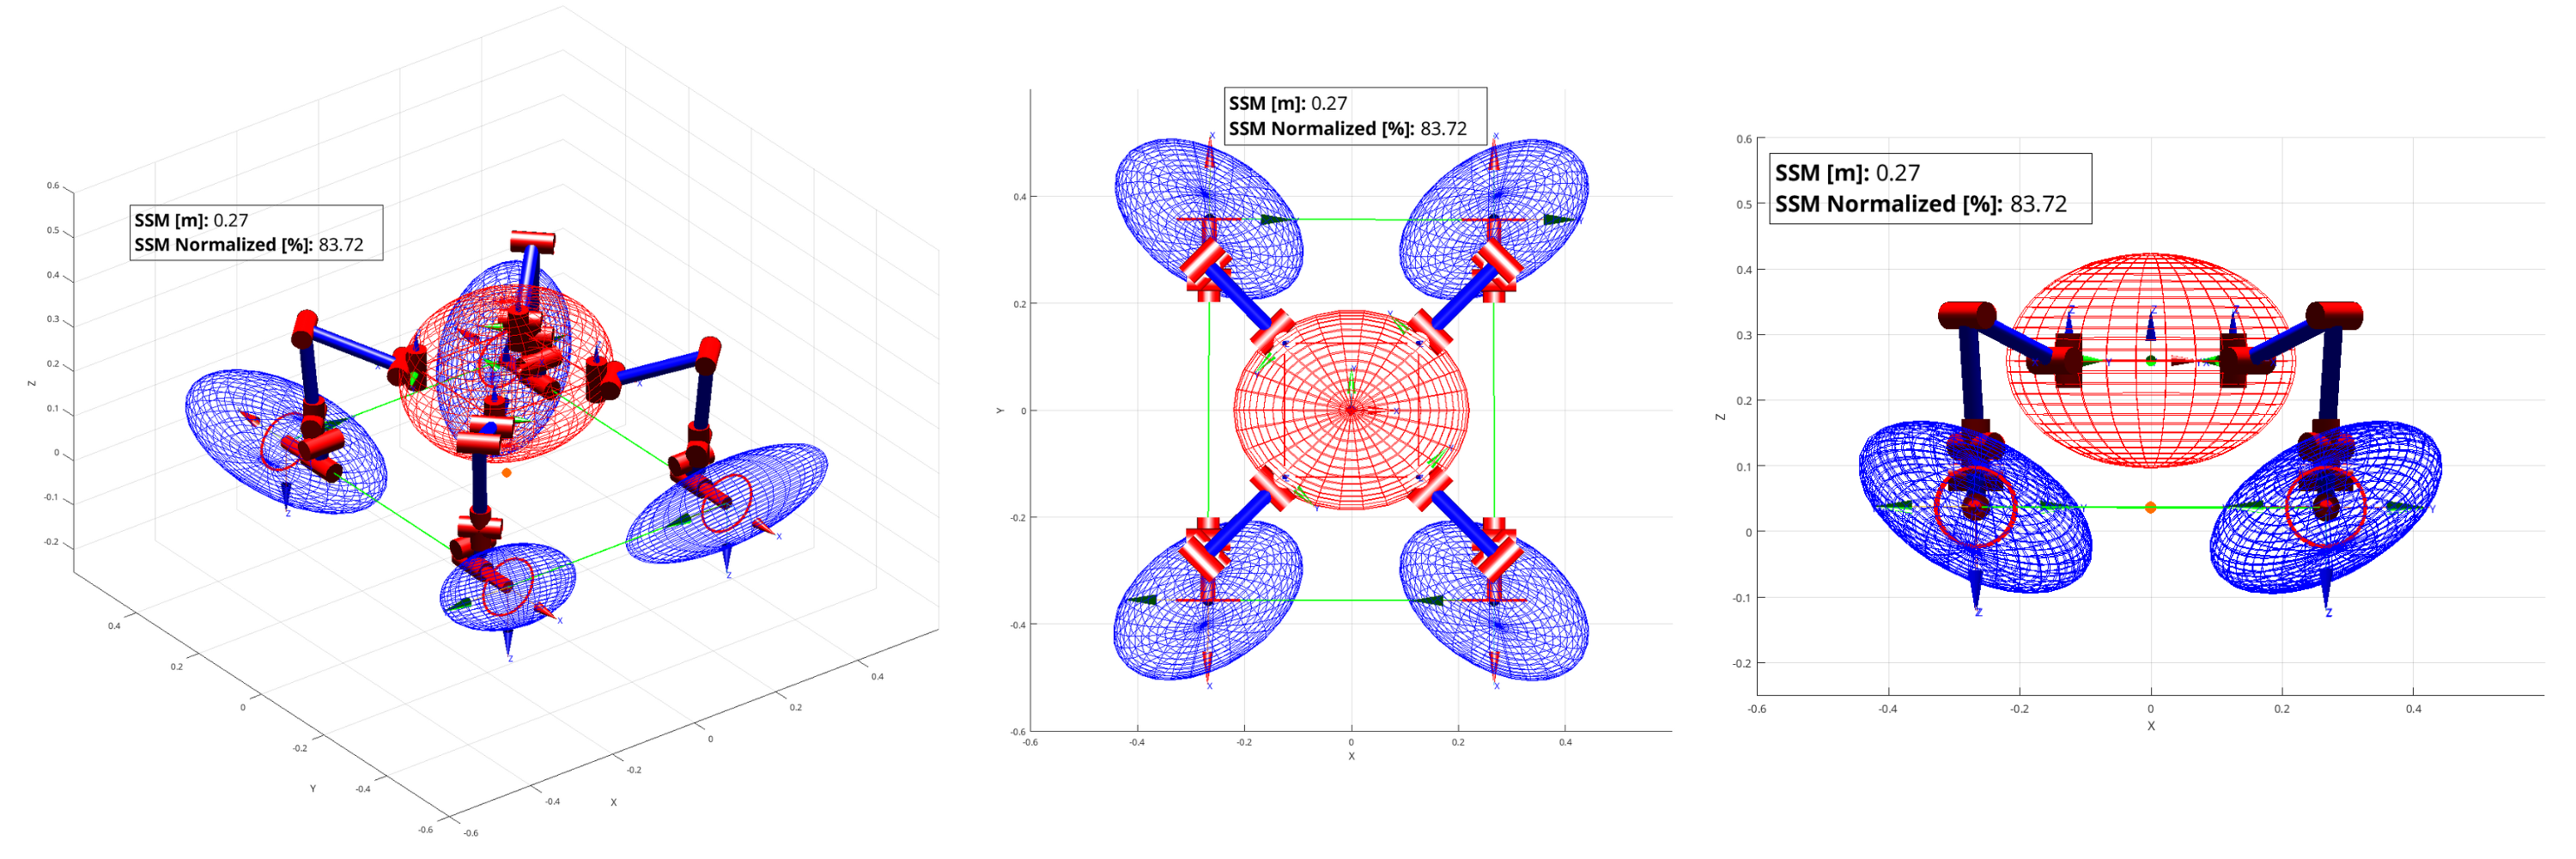
\includegraphics[width=0.9\textwidth]{Images/img_ch5/driving.png}
    \caption{SSM and ATBVME in driving configuration  after G2W transition (perspective, xy, and xz view)}
    \label{fig:Driving_Manipulability}
\end{figure}


\section{Final comments on the Proposed Algorithm}
\label{sec:comments}
In this chapter, a versatile and reliable algorithm to perform the transition of one, multiple, or all modules of LIMBERO-GRIEEL has been defined.
Now some of the comments previously anticipated are discussed, starting from a detailed comparison between the previous and the proposed algorithm


\subsection{Algorithms Comparison}
\label{sec:comparison}

The new algorithm's advantages have additional costs in terms of energy and time required.
The new motion sequence for each module transformation involves one base task (stabilize), two limb tasks (raise and lay down), and one GRIEEL change task (transform). Hence, if a complete locomotion transition is needed, the number of motion tasks involved is higher than that of the previous algorithm. On the other hand, single-limb transitions are faster and less demanding. 
Furthermore, the base motion tasks have been defined to be reliable in the sense of stability, and dexterous in the sense of not wasting motion and maintaining maneuverability, which can reduce the required time and the power consumed. 

Additional experiments and measurements should be done for a quantitative comparison of the two methods in terms of energy consumption. Laying down the base and raising it involves all limb motion, meaning that this qualitative analysis may be wrong. 

 In addition to time and energy considerations, it is important to notice that under some conditions which have been discussed in detail, the old algorithm may cause system failure or damage, in those cases, the proposed one is the clear choice.  

There is no "best" solution for all the conditions, it depends on the environment, the mission requirements, and the available resources. 
Exteroceptive and proprioceptive sensors and mission requirements can be used to infer the optimal choice, enabling multiple transition algorithms instead of prescribing only one possibility.

\subsection{Extensions}
\label{sec:extensions}

Section \ref{sec:new_algorithm} describes the transition sequence for a quadruped robot, moving in an environment where SP criteria and SSM are enough to ensure stability (flat and almost horizontal).

In the algorithm definition, the current locomotion capabilities have been considered, where the robot can walk, climb, or drive with the configurations described in (\ref{sec:locomotion_configurations}). The complex mechanical structure and redundancy of L-G's limbs allow complex locomotion capabilities, and it is interesting to analyze the possible future extensions of the transition algorithm. 

The transformation extensions are briefly discussed for the following cases: working in different terrain conditions, taking advantage of dynamic mode transition or in advanced configurations, and having more than 4 limbs.  

\subsubsection{Different Terrain Conditions}
\label{sec:different_conditions}

In most cases, the assumption of flat and almost horizontal terrain when mode transition occurs can be met, or even imposed, and it is possible to give an intuitive explanation of this. 
When a full locomotion transition occurs, these two cases are the most common: 
\begin{itemize}
    \setlength\itemsep{-0.7em} 
    \item \textbf{Walking to driving}: Locomotion mode transition is considered when moving from a rough terrain to a regular one. This transformation occurs when the terrain changes into a drivable condition, so terrain regularity and negligible slopes are needed. In those conditions, the transformation command is sent when the drivable ground is reached, where SSM is a reliable criterion.   
    \item \textbf{Driving to walking}: When the opposite occurs and motion from drivable to uneven terrain occurs, the transition W2G is enforced before entering the walking zone. 
\end{itemize}

If advanced locomotion and adaptive usage of limbs are considered, the following cases can extend the  transformation scenarios: 
\begin{itemize}
\setlength\itemsep{-0.7em} 
    \item \textbf{Driving on Slopes}: If satisfactory driving performances are met in wheel mode, in terms of traction and reduced slippage, driving on slopes is possible. In those sloped driving cases, the terrain is considered almost flat but not horizontal, then the SSM is not reliable, and the ZMP has to be considered.   
    \item \textbf{Driving exploiting limbs}: Furthermore, if complex limb configurations are considered and adapted to the terrain during driving, the flat ground constraint of wheeled locomotion is no longer necessary\cite{AnymalDocThesis}\cite{MAMMOTH}\cite{WheelLeggedStabilityOPT}. 
    \item \textbf{Dynamic transformation}: As discussed in the next section, complex robot configuration may occur during the transition when the full system's potential is exploited. 
    The terrain can be irregular, the inertial effect non-negligible, and the gripping forces relevant. 
\end{itemize} 

In those scenarios, the SSM is unreliable (as discussed in chapter \ref{ch:chapter_three}), and more advanced stability criteria like the ZMP, TSM, or GIA are better choices. 

Thanks to the modularity of the proposed transition algorithm, integrating different stability criteria is possible. After classifying the terrain condition and the contact points/forces, the base translation is defined accordingly, and stability can be ensured. 

\subsubsection{Hybrid locomotion and Dynamic Transition}
\label{sec:different_conditions}

Understanding what is and when hybrid locomotion is possible serves the purpose of introducing another possible condition where module transition may be exploited. 

Previously the term "hybrid configuration" has been used to indicate a configuration in which the robot has different types of EE during task execution. \textit{Hybrid locomotion} instead, indicates the type of locomotion where an EE built for a specific function is used differently. An example is walking with wheeled limbs (locking the driving joints in the meantime), and researchers at ETH proved with ANYmal on wheels\cite{AnymalDocThesis}that this is possible and enables new capabilities. 

While a multi-limbed robot with GRIEEL can transform the locomotion module, in most conventional robots either wheels or gripper/foot are mounted. The considerations of the different locomotion efficiency (behind the development of GRIEEL) explain why walking locomotion with wheeled legs has been studied \cite{AnymalDocThesis}\cite{WheelLegged}.

The main problem with wheeled walking locomotion is that some terrains are completely unfeasible to walk in using a wheel-shaped foot. In those contexts, GRIEEL multimodality surpasses every other system.
However, implementing a possible walking wheeled gait with GRIEEL can further increase the potentiality of the system, for example: 
\begin{itemize}
    \setlength\itemsep{-0.7em} 
    \item \textbf{Obstacles when driving while manipulating}: When LIMBERO-GRIEEL (or any quadruped limbed-robot using GRIEEL) is in a hybrid configuration, on three wheels and the last limb carrying an object, the global path to the goal location has to be planned considering only driving locomotion. If a locomotion transition is needed on a small portion of the path, and the base cannot be supported on the ground, the object has to be temporarily dropped to ensure three points of contact during limb transformation. If instead, the roughness of the terrain is such that walking wheeled can be considered in those critical points, mission time and effort are significantly reduced. 
    \item \textbf{Few obstacles on the driving path}: In conditions similar to the one listed above, where wheeled locomotion is feasible along the path, except for a small portion. When that portion allows hybrid locomotion, maintaining wheel mode is probably the most efficient solution.   
\end{itemize}

Those considerations require complex path planning and decision-making, based on terrain traversability analysis, global cost maps, and representative cost functions. The description of such algorithms and procedures is above the scope of this research, but it is a required capability to enable system autonomy to exploit its full potential.  

Considering also hybrid locomotion, it is possible to extend the possible module transition to dynamic conditions: 
\begin{itemize}
    \setlength\itemsep{-0.7em} 
    \item \textbf{Transition during locomotion}: In case the transition occurs during a path-following task, the transition sequence has been defined as a pause on the path execution. It is possible to redefine that single module transformation (\ref{alg:single_grieel_transition}) as part of a limb trajectory during a walking step. With this approach, when a full locomotion transition is needed, additional steps toward the final location can be completed during mode transformation.  \item \textbf{Hybrid locomotion recovery}: When hybrid locomotion is in execution, but criticality occurs because of inaccurate planning, a transition to gripper mode has to start
    \item  \textbf{Driving to climbing}: If a transition from driving to climbing locomotion is imminent, it is possible to perform motions to start climbing during transformation. For example, the front limbs are positioned closer to the climbing wall, and during W2G the grippers are directly attached to the wall instead of laying it back on the ground. 
\end{itemize}

The advanced tasks and possibilities described above are interesting aspects, which require a complex and adaptable control system. 
However,  in terms of the module transition, the reusability of the single transformation can be exploited, defining additional components that account for adaptable limb and base tasks. 

\subsubsection{N-limbed Robots}
\label{sec:N_limbed_extension}

GRIEEL has been tested and analyzed as an extension of LIMBERO's limbs, however, its final purpose is to become a reusable module to be integrated into different limbed robots. The mechanical design is already independent of the limb, but additional efforts will be necessary to make its control software modular and reusable.

The details on this reusability design requirements are out of this research scope. It is interesting to analyze the additional considerations and functionalities the transition algorithm should integrate when GRIEEL is attached to a robot with more than 4 limbs. 

Legged robots are commonly designed with an even number of legs (bipeds, quadrupeds, hexapods,\dots), because of symmetry and periodic gait scheduling. 
Having a transformable module enables additional functionalities, for example, a quadruped limbed robot with GRIEEL as EE can mount a supplemental lighter limb, this can be retracted above the body if properly designed, and extracted for object manipulation or additional driving/walking support in critical conditions. 

In a six-limbed robot (such as SCAR-E \cite{SCAR-E}), by attaching GRIEEL as EE it is possible to exploit the additional stability of more contact points (bigger SP) for manipulation tasks. 
The hybrid configuration previously discussed for L-G here is even more functional, four limbs can be used in driving mode, and two adjacent limbs in gripper mode, enabling cooperative manipulation with two "arm-like" limbs \cite{CooperativeManipulators}. 
Additionally, having 6 wheels provides higher traction force, with the possibility of driving in steeper terrains. 

In terms of the GRIEEL transition algorithm, it is clear that having six possible points of contact makes the single-limb transition much easier. The case of 6-wheeled to 4-wheeled + 2-gripper is easily managed by keeping the 4-wheeled limbs on the ground and raising the ones to transform (taking into consideration inertial and gravitational effects if affecting the system stability, for example when quick motions are involved or when the limbs are heavy). 

Fig.\ref{fig:sixlimbsGRIEEL} represent conceptually different configurations and functionalities for a robot with six limbs equipped with GRIEEL.


\begin{figure}[H]
    \centering
    \subfloat[hexapod LIMBERO-GRIEEL in Gazebo mars world .\label{fig:hexapod_mars}]{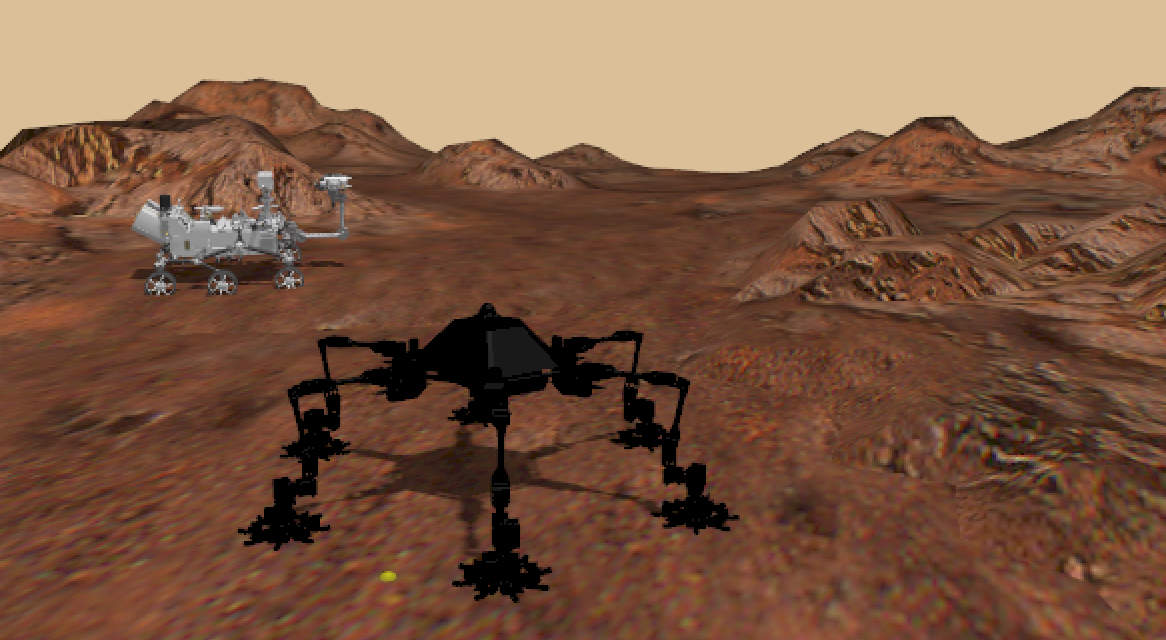
\includegraphics[width=0.7\textwidth]{Images/img_ch5/hexapod_mars.png}} \quad 
    \\
    \subfloat[Gripper mode\label{fig:hexapod_gripper}]{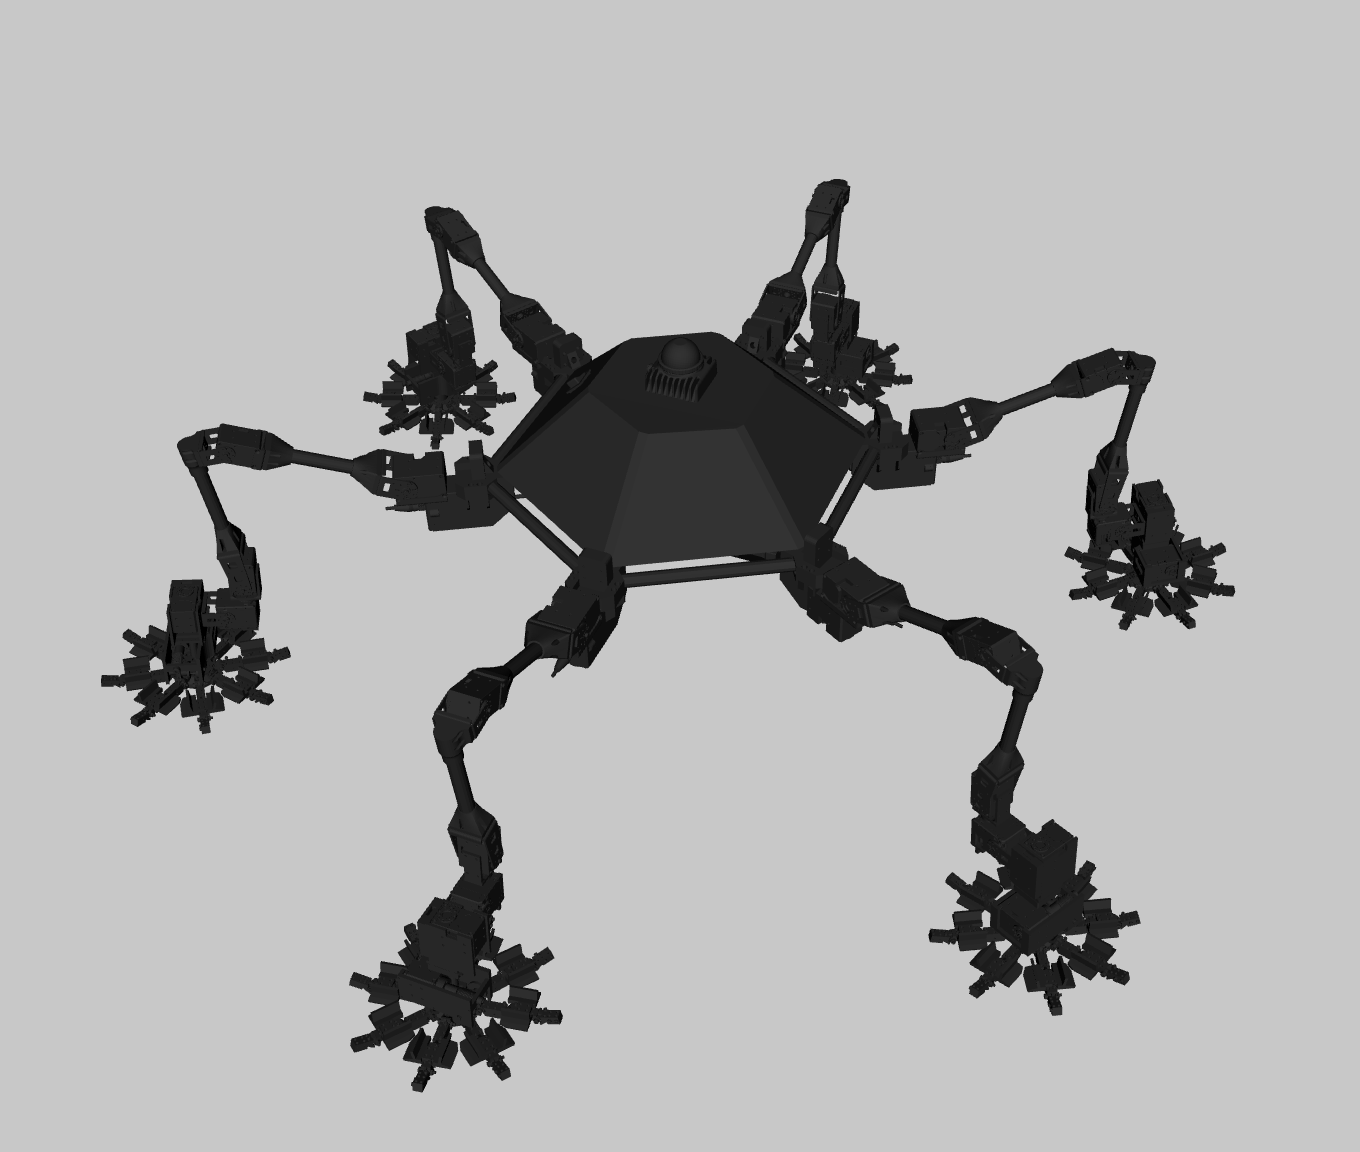
\includegraphics[width=0.38\textwidth]{Images/img_ch5/hexapod_gripper.png}}\quad
    \subfloat[Wheel mode\label{fig:hexapod_wheeled}]{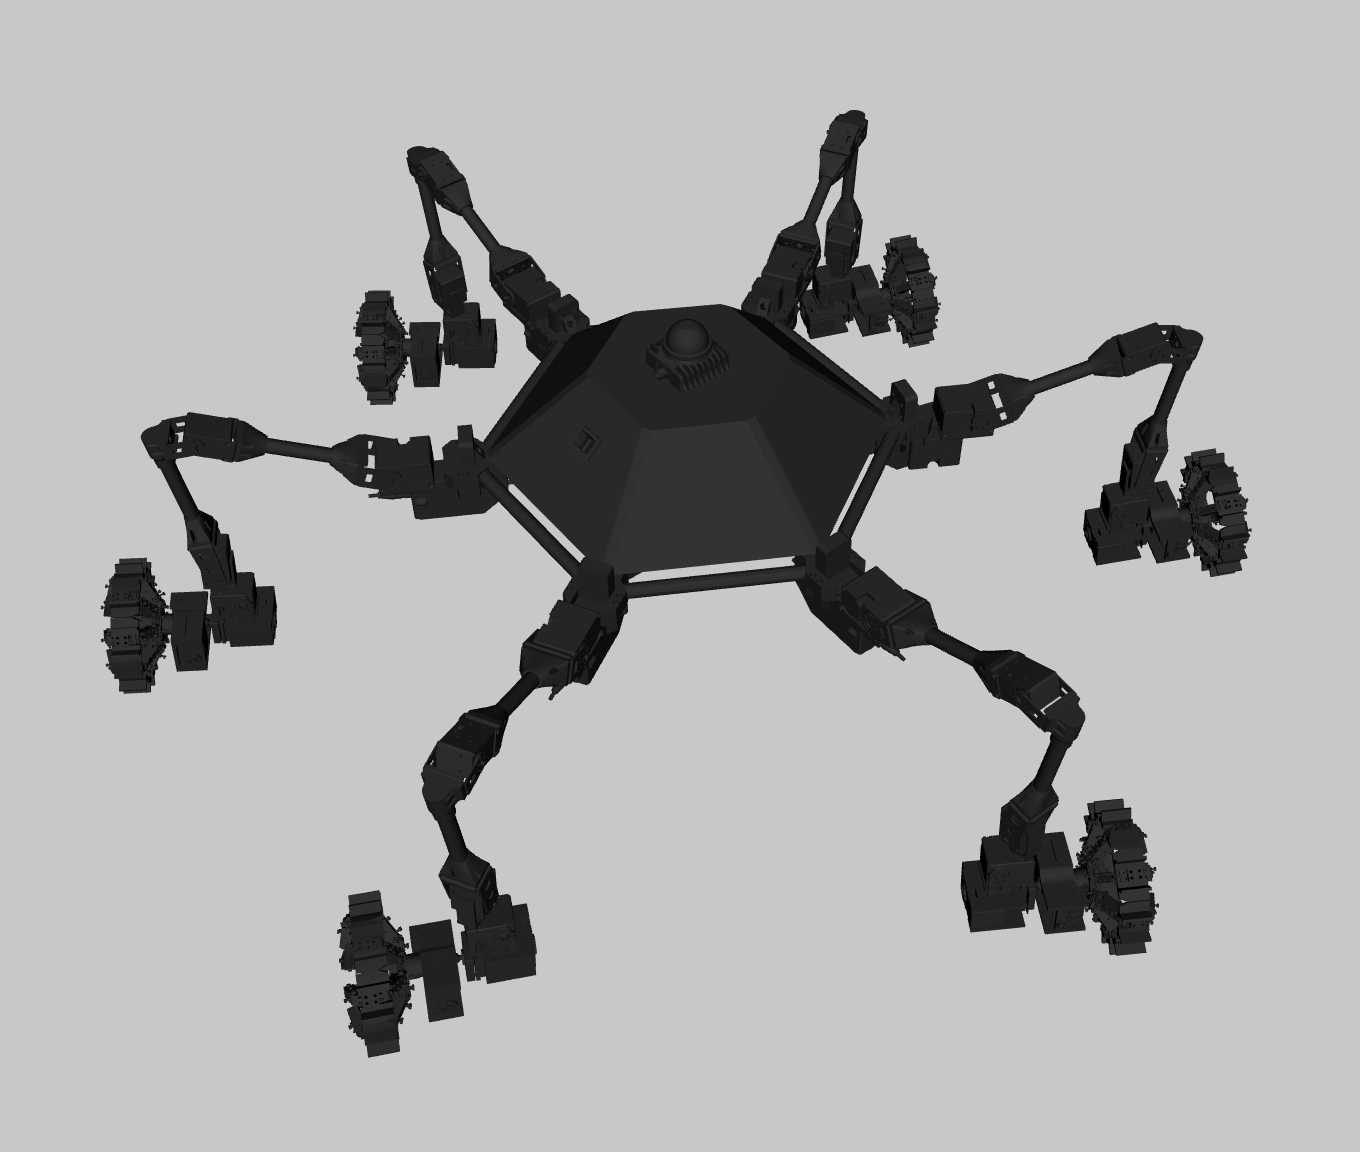
\includegraphics[width=0.38\textwidth]{Images/img_ch5/hexapod_wheeled.png}}\quad
    \\
     \subfloat[Hybrid cooperative frontal  grippers\label{fig:hexapod_manipulate}]{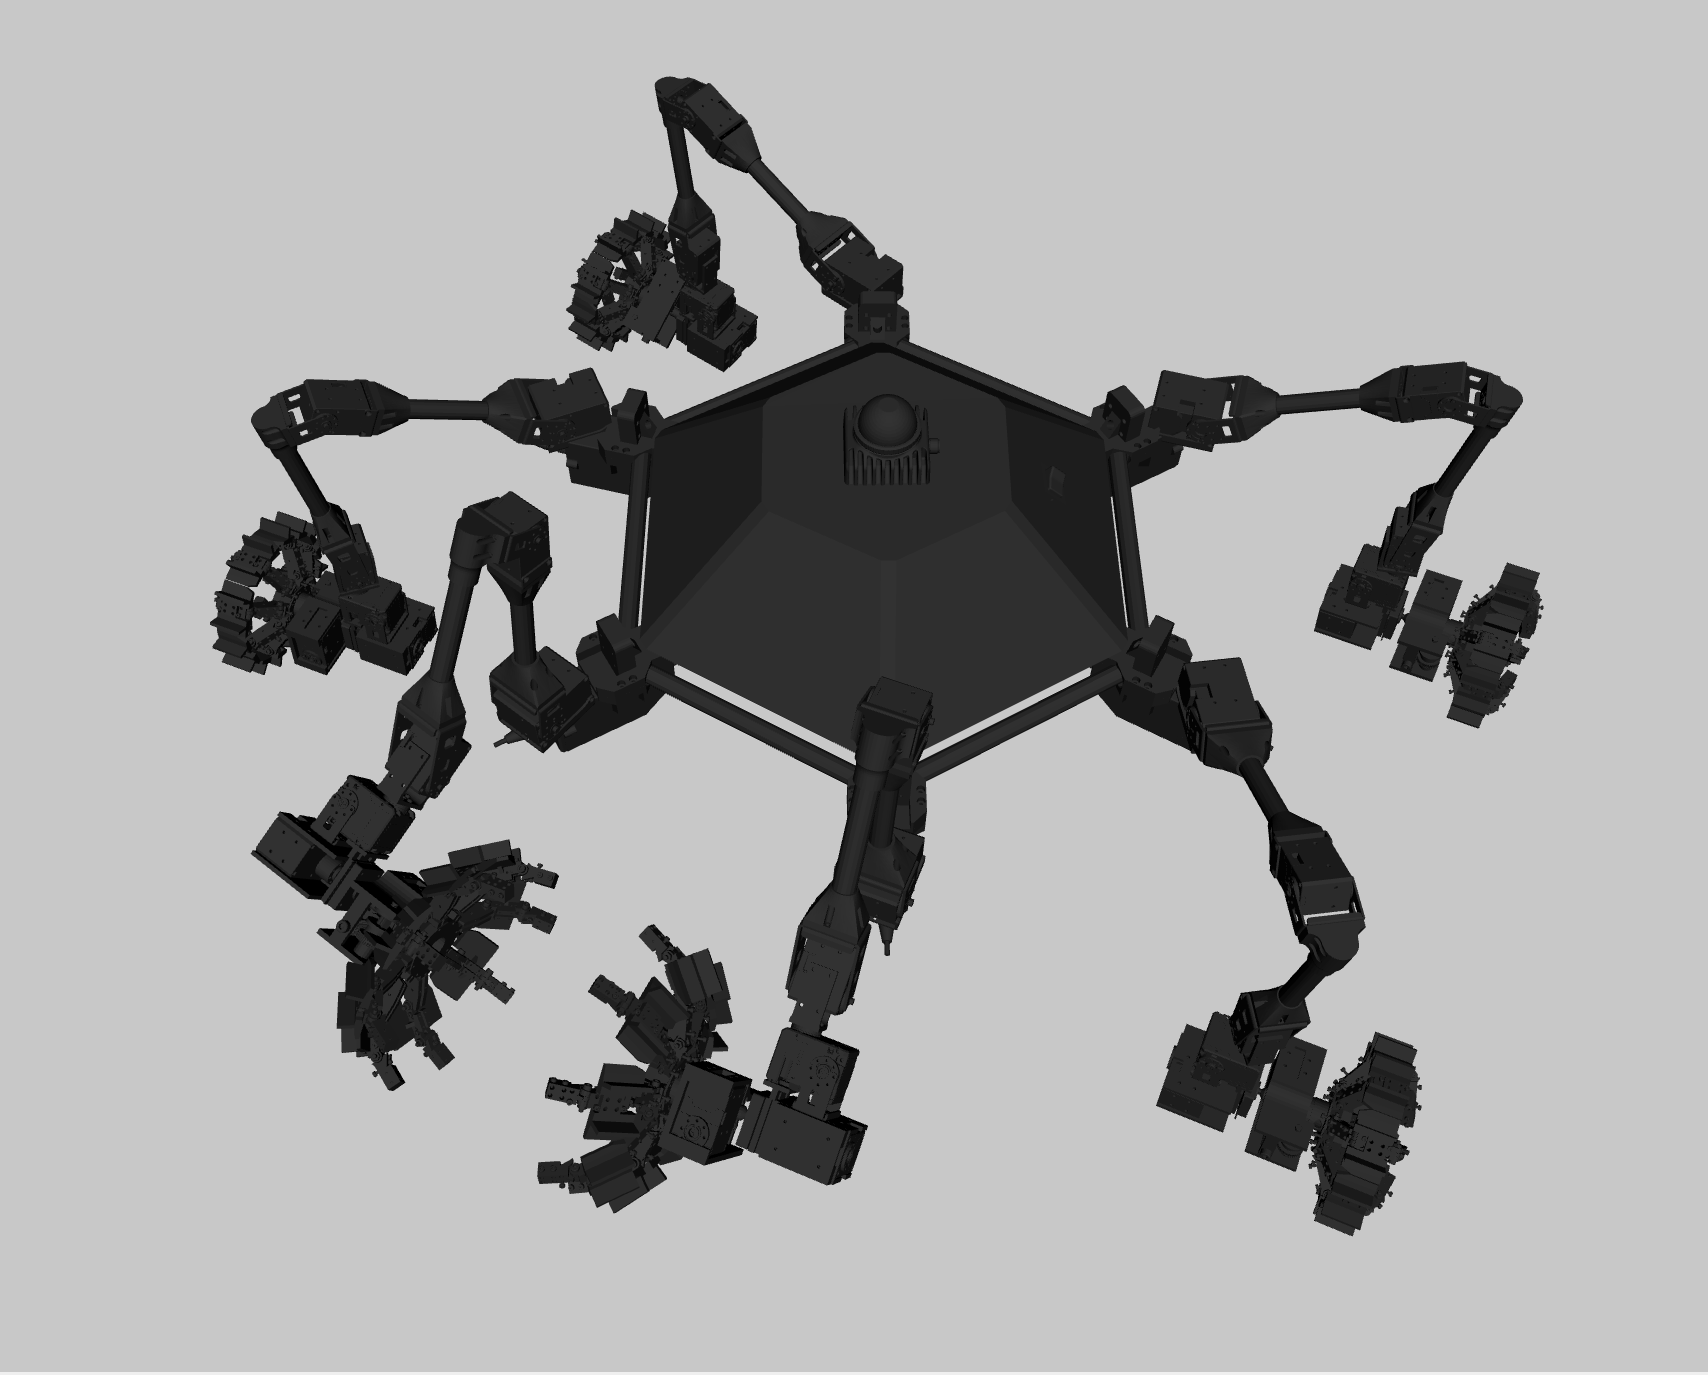
\includegraphics[width=0.38\textwidth]{Images/img_ch5/hexapod_manipulate.png}}\quad
    \subfloat[Hybrid side grippers\label{fig:hexapod_manipulate_side}]{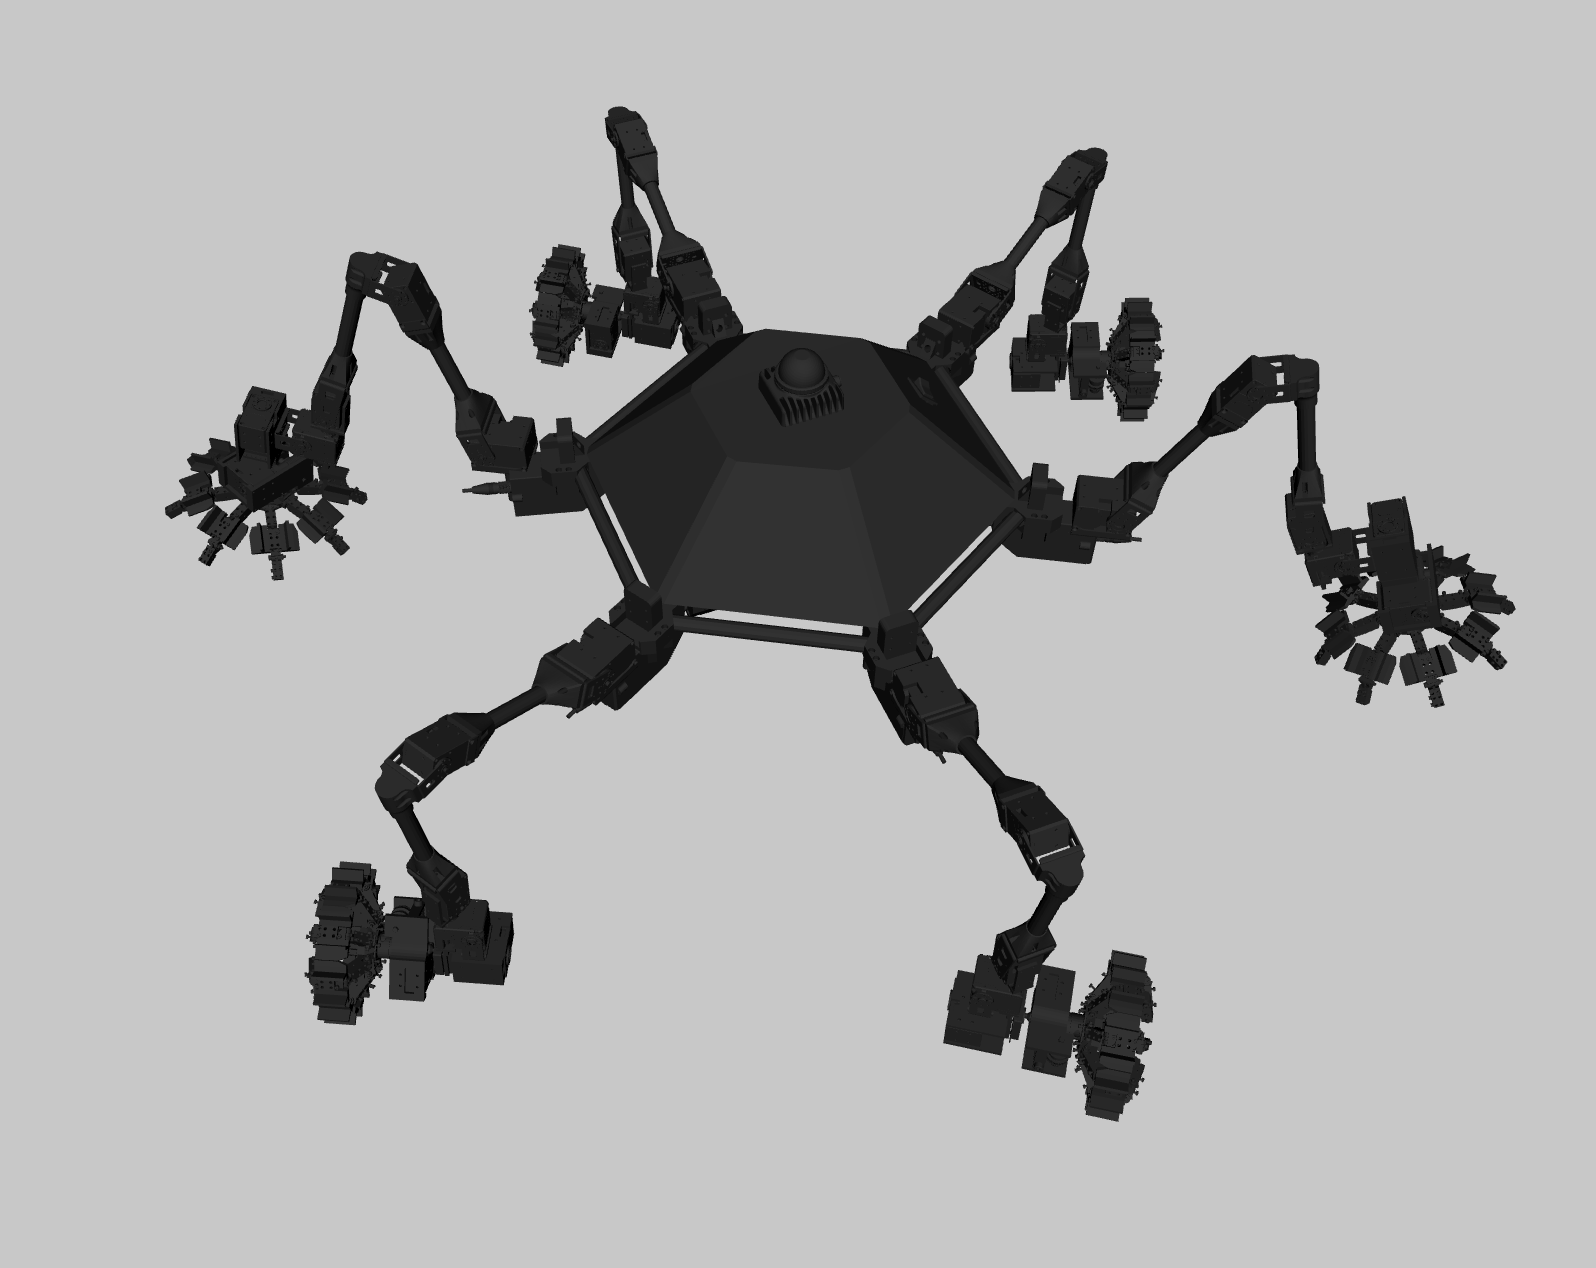
\includegraphics[width=0.38\textwidth]{Images/img_ch5/hexapod_manipulate_side.png}}\quad   
    \caption[Conceptual representation of hexapod LIMBERO-GRIEEL]{Hexapod LIMBERO-GRIEEL in different configurations}
    \label{fig:sixlimbsGRIEEL}
\end{figure}